\documentclass[a4paper]{report}
% \documentclass[a4paper,twoside,openright]{report}
% \documentclass[a4paper]{book}

% \linespread{1.25}

%% listado de código
%% https://es.wikibooks.org/wiki/Manual_de_LaTeX/Listados_de_c%C3%B3digo/Listados_con_listings
\usepackage{listings}
\lstset{literate=
  {á}{{\'a}}1 {é}{{\'e}}1 {í}{{\'i}}1 {ó}{{\'o}}1 {ú}{{\'u}}1
  {Á}{{\'A}}1 {É}{{\'E}}1 {Í}{{\'I}}1 {Ó}{{\'O}}1 {Ú}{{\'U}}1
  {à}{{\`a}}1 {è}{{\`e}}1 {ì}{{\`i}}1 {ò}{{\`o}}1 {ù}{{\`u}}1
  {À}{{\`A}}1 {È}{{\'E}}1 {Ì}{{\`I}}1 {Ò}{{\`O}}1 {Ù}{{\`U}}1
  {ä}{{\"a}}1 {ë}{{\"e}}1 {ï}{{\"i}}1 {ö}{{\"o}}1 {ü}{{\"u}}1
  {Ä}{{\"A}}1 {Ë}{{\"E}}1 {Ï}{{\"I}}1 {Ö}{{\"O}}1 {Ü}{{\"U}}1
  {â}{{\^a}}1 {ê}{{\^e}}1 {î}{{\^i}}1 {ô}{{\^o}}1 {û}{{\^u}}1
  {Â}{{\^A}}1 {Ê}{{\^E}}1 {Î}{{\^I}}1 {Ô}{{\^O}}1 {Û}{{\^U}}1
  {ã}{{\~a}}1 {ẽ}{{\~e}}1 {ĩ}{{\~i}}1 {õ}{{\~o}}1 {ũ}{{\~u}}1
  {Ã}{{\~A}}1 {Ẽ}{{\~E}}1 {Ĩ}{{\~I}}1 {Õ}{{\~O}}1 {Ũ}{{\~U}}1
  {œ}{{\oe}}1 {Œ}{{\OE}}1 {æ}{{\ae}}1 {Æ}{{\AE}}1 {ß}{{\ss}}1
  {ű}{{\H{u}}}1 {Ű}{{\H{U}}}1 {ő}{{\H{o}}}1 {Ő}{{\H{O}}}1
  {ç}{{\c c}}1 {Ç}{{\c C}}1 {ø}{{\o}}1 {å}{{\r a}}1 {Å}{{\r A}}1
  {€}{{\euro}}1 {£}{{\pounds}}1 {«}{{\guillemotleft}}1
  {»}{{\guillemotright}}1 {ñ}{{\~n}}1 {Ñ}{{\~N}}1 {¿}{{?`}}1 {¡}{{!`}}1 
}

%% Spanska!
\usepackage[utf8]{inputenc}
\usepackage[T1]{fontenc}    % 8-bit encoding. Acentuados como único caracter.
\usepackage[spanish]{babel}
% \def\spanishoptions{argentina}

%% graphics
\usepackage{graphicx}
\graphicspath{ {./graphs/} }
\usepackage{wrapfig}
\usepackage{tikz}

%% biblatex
% \usepackage[style=custom-numeric-comp, backend=biber, sorting= none, url= true, maxnames=20]{biblatex}
\usepackage[style=numeric, backend=biber, sorting= none, url= true, maxnames=20]{biblatex}
\DefineBibliographyStrings{spanish}{}
\usepackage{csquotes}
\usepackage{textgreek} % https://tex.stackexchange.com/questions/107352/non-ascii-characters-in-biblatex 
\addbibresource{sismos.bib}

%% physics
\usepackage[separate-uncertainty=true, locale=FR]{siunitx}

%% vínculos en documento pdf
\usepackage{hyperref}
\usepackage[all]{hypcap}
\hypersetup{
    colorlinks=false    % false:boxedlinks ; true:coloredlinks
}

%% tablas
\usepackage{booktabs}

%% matemática
\usepackage{amsmath} % aligned

%% color text
\usepackage{xcolor}



\begin{document}

%\title{
%	{Factores físicos de los terremotos que influyen en su percepción por la población}\\[1 cm]
%	{Trabajo final de la asignatura ``Taller de tesis''}
%	{
\includegraphics[width=\textwidth]{logos}}
%}
%\author{Víctor A. Bettachini}
%\date{\today}
%\maketitle
%
%\begin{abstract}
%	Niente.
%\end{abstract}


% Title page
\begin{titlepage}
    \centering
    %\vspace*{1in}
    
    \huge\textbf{Predicción de la percepción de sismos por la población a partir de datos básicos de terremotos}
    
    \vspace{0.5in}
		Trabajo final de la asignatura\\``Taller de tesis''\\
    \vspace{0.5in}
		
\includegraphics[width=\textwidth]{logos}\\
    \vspace{0.5in}
    
    \large
    \textbf{Autor:}\\
		Víctor A. Bettachini\\
    \vspace{0.5in}
    \textbf{Fecha:}\\
    \today
    
    \vfill
    \begin{minipage}{0.8\textwidth}
    \begin{abstract}
        Una decena de terremotos se producen en el territorio nacional en forma diaria sin que sean detectados más que por instrumentos.
				Son muy pocos los casos en que las ondas sísmicas que estos producen son percibidos por la población.
				Se buscó desarrollar un modelo para predecir tal eventualidad utilizando usando solo datos básicos de terremotos.
				Limitaciones de los datos públicos utilizados limitaron el espacio geográficos del estudio a la provincia de San Juan.
				Se ensayaron modelos basado en regresión logística como uno basado en máquinas de potenciación de gradiente.
				Se logró ajustar modelos con alternativamente alta sensibilidad o precisión, pero no ambas simultáneamente, por lo que se debe optar entre estas alternativas según cual sea la prioridad para la aplicación que quiera dárseles.
				% Algo de resultados
    \end{abstract}
		\end{minipage}
	\end{titlepage}

\tableofcontents

% \mainmatter

\chapter{Introducción}

\section{Contexto y motivación científica}\label{sec:contexto}

Un rápido desprendimiento entre dos facetas enfrentadas de sendas placas tectónicas que se traban mutuamente su desplazamiento relativo produce una rápida liberación de energía que se denomina terremoto.
Esto sucede a cierta profundidad en la corteza terrestre en el punto denominado hipocentro a partir del cual parte de esta energía se encauza como ondas elásticas.
El estudio de estas ondas es el área llamada sismología y de ahí el termino sismo para un evento particular detectado, pero que debiera aclararse si se produjo por un terremoto u otra fuente de ondas \cite[sección 4.1.1]{fowler_solid_1990}.

\begin{figure}[!ht]
% \begin{wrapfigure}[15]{r}{0.4\textwidth}
  \centering
	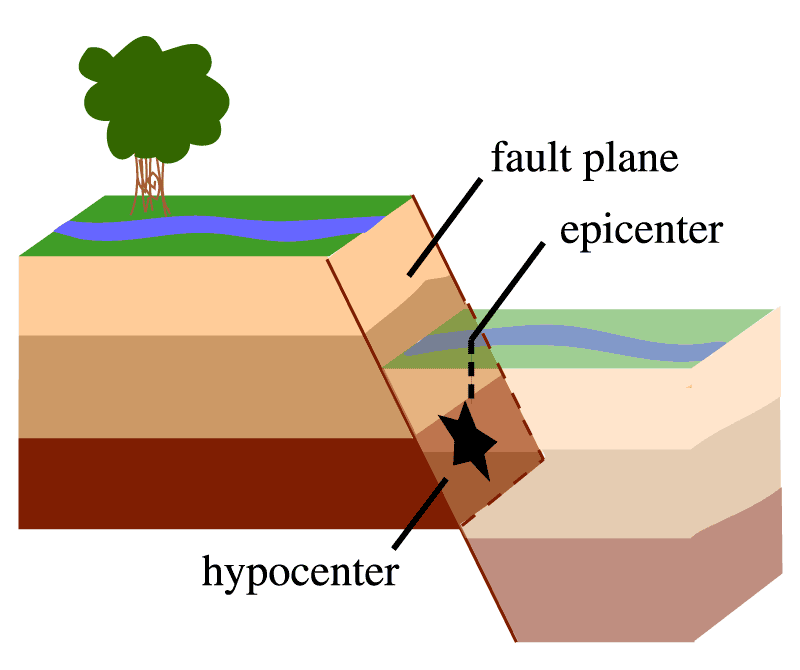
\includegraphics[width=0.6\textwidth]{eq-ed-fault-labeled.png}
	\caption{El epicentro es el punto de la superficie inmediatamente sobre el hipocentro que es el punto a cierta profundidad al que se adscribe un terremoto.
	Reproducido de \cite{lisa_wald_science_nodate}.
	}
	\label{fig:epicentro_hipocentro}
% \end{wrapfigure}
\end{figure}

Sean las generadas ondas de compresión longitudinal de la corteza, las tipo P, o las del tipo S, transversales y más lentas, ambas arriban con mayor intensidad al punto de la superficial terrestre que se encuentra directamente sobre el hipocentro, que se denomina epicentro \cite[sección 4.1.2]{fowler_solid_1990} como ilustra la figura \ref{fig:epicentro_hipocentro}.
Cuanto más próximo es un punto en la superficie al hipocentro, la amplitud de las ondas sísmicas registradas en la superficie es mayor.
Tanto esta amplitud como el período de oscilación son mucho mayores que el de otros desplazamientos de la corteza como los de las mareas solares y lunares de la corteza \cite[sección 4.1.4]{fowler_solid_1990}.
Como resultado, estructuras artificiales pueden agitarse poniendo en riesgo su estabilidad estructural y haciendo caer elementos que no estaban fijados a esta o perdieron tal adhesión a causa de la agitación misma.
Como consecuencia, los sismos más fuertes pueden generar graves daños, poniendo en riesgo la integridad física y la seguridad de las personas al generar daños en las viviendas y edificios, derrumbes de puentes, rompimiento de vidrios, entre otros \cite{noauthor_que_2018}.

La mayor parte de los sismos presentan ondas de pequeña amplitud y no generan daños materiales.
Que sean o no detectados por la población es un factor relevante en su percepción de confianza vis-à-vís de los organismos de monitoreo y prevención de riesgos.
Cuando informar a la población de la ocurrencia de un sismo es una decisión de política pública que debiera apuntar a no alertar innecesariamente sobre sismos menores imperceptibles \cite{saunders_j_k_twist_nodate}.
El caso inverso es también problemático, en que ante una carencia de una comunicación oficial de la poca importancia de un evento sísmico llevó a la autoevacuación por parte de la población que lo percibió \cite{vaiciulyte_population_2022}. 



\section{Objetivos del trabajo / Pregunta}\label{sec:objetivo}

Contar con una estimación rápida a partir de los datos sísmicos registrados por instrumental de si un dado evento será percibido por la población o no permitiría a las autoridades tomar decisiones informadas sobre la comunicación a la población.
Este trabajo busca determinar el grado de certeza con que ciertos métodos de ciencias de datos pueden predecir si la población percibirá actividad sísmica producto de terremotos a partir de unos pocos datos básicos sobre los mismos publicados por el Instituto Nacional de Prevención Sísmica (INPRES) que es el organismo público de la República Argentina que realiza estudios e investigaciones básicas y aplicadas de sismología \cite{noauthor_instituto_2022}.



\section{Estructura del documento}

Se estructuró en los siguientes capítulos con temáticas diferenciadas
\begin{description}
	\item[Introducción]: se presentará el contexto y la motivación científica, los objetivos del trabajo y la estructura del documento.
	\item[Marco teórico]: se revisarán los trabajos previos y relevantes, se presentarán los conceptos y técnicas de ciencia de datos utilizados en el trabajo.
	\item[Metodología]: se describirán los datos utilizados, el preprocesamiento y limpieza de los mismos, el análisis exploratorio de los datos, las técnicas de análisis y modelado utilizadas, la selección de características, las métricas de evaluación de los modelos y los métodos estadísticos utilizados.
	\item[Resultados y discusión]: se presentarán y analizarán los resultados obtenidos, se discutirán los resultados y su relevancia, se identificarán las limitaciones y posibles mejoras.
	\item[Conclusión]: se resumirán los hallazgos principales, se presentarán las conclusiones generales y su relación con los objetivos del trabajo, se discutirán las aplicaciones y relevancia de los resultados.
\end{description}



\chapter{Marco teórico}


\section{Relevamiento de trabajos previos y relevantes}

%La problemática de la percepción por la población de un terremoto tal vez deba separarse en dos problemas a resolver secuencialmente.
%En primer lugar, determinar el espectro de frecuencias de oscilación del suelo, el sismo, en función de características físicas del terremoto y la corteza.
%Y en segundo lugar, la respuesta de las personas a tal espectro de oscilaciones que depende, además de características de las viviendas, de cuestiones fisiológicas.
%
%Para la predicicción del espectro de oscilaciones existen probados conjuntos de ecuaciones determinísticas en función de la distancia al hipocentro y características de la corteza en el camino de propagación de las ondas desde el terremoto.
%Los correspondientes factores deben ajustarse para cada localización, y no es infrecuente que se carezca de parte de la información requerida, usalmente la referida a la geología local \cite{lior_relation_2018} 
%Ante esta problemática, y como alternativa a enfoques determísticos, se han ensayado técnicas de aprendizaje automático, y en años recientes, arquitecturas de redes neuronales recurrentes \cite{datta_deepshake_2022}.
%
%La respuesta fisiológica a oscilaciones del suelo es central en la muy activa área de la predicción de terremotos de gran importancia basada en la capacidad sensorial, pero no de humanos, sino la de animales.
%Hay una abultada historia de observaciones que avalan que muchos animales son sensibles a señales que dan alarma anticipada de próximos sismos \cite{kirschvink_earthquake_2000}.

En la prensa general se busca transmitir la importancia de un fenómeno sísmico informando un valor sea en la escala de Richter o de Mercalli como si fueran intercambiables.
La primera se refiere a la magnitud, una característica física del terremoto (ver definición en la sección \ref{sec:ingeniería}), en tanto que la segunda se refiere a una caracterización subjetiva del sismo, la llamada intensidad.
Esta última cantidad es función de fenómenos percibidos por el público como si hubo grietas en el suelo o vidrios o si temblaron edificios \cite[sección 4.2.3]{fowler_solid_1990}.
% Como tal es una caracterización posterior al fenómeno por lo que su valor numérico no es útil a los efectos del objetivo descripto en la sección \ref{sec:objetivo}.
Los organismos de monitoreo de sismos cuentan con portales en la world-wide web para que el público ofrezca tal información voluntariamente en formularios con preguntas de elección múltiple.
Tal es el caso de los portales ``Encuesta de sismos'' del INPRES \cite{noauthor_encuesta_nodate} y ``Felt Report - Tell Us!'' \cite{noauthor_felt_nodate} parte del programa de riesgo de terremotos del Geological Survey de los Estados Unidos de América (USGS) \cite{david_jay_usgs_2012}. 
Este último aporta a la sistematización de reportes del público denominado ``Did you fell it?'' (DYFI) que ha nutrido en la último década y media a varios estudios relacionando la intensidad con diversos fenómenos citados en \cite{noauthor_dyfi_nodate}.

La intensidad expresada en la escala modificada de Mercalli (MMI) \cite{noauthor_intensidad_2022} en la base de datos DYFI mostró estar bien correlacionada con medidas de espectro de oscilación lo que impulsó a buscar un modelo que le relacione con parámetros físicos de terremoto.
Una regresión múltiple basada en el método de máxima verosimilitud se encontraron los factores \(c_{1\dots7}\) de la \cite[ecuación 1]{atkinson_did_2007}
\begin{equation}
	MMI = c_1 + c_2 (M_w - 6) + c_3 (M_w - 6)^2 + c_4\log{R} + c_5 R + c_6 B + c_7 M_w \log{R}, 
	\label{eq:atkinson2007}
\end{equation}
donde \(M_w\) es la magnitud del momento, según la definición discutida en la sección \ref{sec:magnitud}, \(R = \sqrt{D + h}\) es la distancia entre observador e hipocentro en función de la distancia del primer al epicentro \(D\) y profundidad del segundo \(h\), y \(B\) es nulo para \(R < R_t\) una distancia de transición en la forma de atenuación de las ondas 
Una posterior actualización de este modelo por los mismos autores se basó en agrupar los valores promedio de MMI en cada código postal
\begin{equation}
	MMI = c_1 + c_2 M_w + c_3 \log{R} + c_4 R + c_5 B + c_6 M_w\log{R},
	\label{eq:atkinson2014}
\end{equation}
con \(R = \sqrt{D + h + 14^2 }\) donde el factor adicional, \(14^2\) da cuenta de la saturación a cortas distancias permitiendo simplificar el factor \(B = \text{máx}(0, \log(R/50))\) que ya no requiere establecer un valor de transición \(R_t\) \cite{atkinson_intensity_2014}. 
	
Lo anterior muestra que hay antecedentes de que un ajuste permite predecir la percepción de los mismos por parte de la población a partir datos físicos de los terremotos 
Para este trabajo lo que busca determinarse es una decisión binaria entre lo que correspondería a la intensidad 0 y 1 de la escala MMI, respectivamente una percepción solo con instrumentos o una por al menos una fracción de la población \cite{noauthor_intensidad_2022}.
No es el enfoque a seguir discriminar con un umbral tras una predicción del valor MMI sino utilizar las técnicas de aprendizaje automático que generen una decisión binaria directamente desde los datos de parámetros físicos.

% La aplicación más usual de herramientas de aprendizaje automático a la temática de terremotos ha perseguido la históricamente esquiva predección de sismos de gran magnitud \cite{allie_hutchison_how_2023}.
% En menor medida presiguen mejoras en la precisión y exactitud en la detección a través de mejoras en el análisis de datos generados por el instrumental.

% Applying Machine Learning to Earthquake Engineering: A Scientometric Analysis of World Research \cite{hu_applying_2024}.

%Un trabajo interesante, no porque sea un antecedente del enfoque o temática de este trabajo pero sí por tocar al aspecto social de la percepción de sismos, hace uso del método conocido como SHAP (contracción de SHapley Additive exPlanations, explicaciones aditivas de Shapley) que determina la contribución de cada característica en un conjunto de datos a una determinada predicción \cite{molnar_96_2024}.
%Los datos son características sociológicas de los individuos y la predicción es sobre la percepción personal del riesgo sismológico.
%Los autores muestran un resultado estadístico que avala el que se incrementa la percepción del riesgo de esta fuente tras haber percibido un sismo \cite{bedle_recognizing_2022}.




\section{Conceptos y técnicas de ciencia de datos utilizados en el trabajo}

% Siendo el objetivo de cualquier modelo utilizado una clasificación entre dos clases, la percepción de un sismo o no, se busca determinar que tan fuerte es el vínculo de cada una de las variables de los sismos de las que se dispone datos y la percepción de los mismos por parte de la población.

Se utilizan en este trabajo dos técnicas con aplicación a la predicción pero en sendos extremos de complejidad y transparencia en cuanto al peso relativo que tienen las variables independientes en el resultado, el de regresión logística y el de máquinas de potenciación de gradiente, más conocidos por su nombre en inglés Gradient Boosting Machines (GBM).


\subsection{Regresión logística para la predicción binaria}\label{sec:logística}

Lo siguiente es un resumen del material de la novena clase de la asignatura \emph{Enfoque estadístico del aprendizaje} titulada \emph{Regresión Logística} elaborado por Juan Barriola, Azul Villanueva y Franco Mastelli. 

Un modelo de regresión lineal con coeficientes \(\beta_j\) para cada variable \(X_j\) que busque la probabilidad de una dependiente binaria \(P(Y)\)  
\begin{equation}
P(Y) = \beta_0 + \sum\limits_{j=1}^p \beta_j X_j,	
\end{equation}
no presentaría un punto de corte claro para clasificar los datos en dos categorías.
Para sortear esta dificulta se toma la salida de esta regresión como la variable dependiente de una regresión logística,
\begin{equation}
P(Y|X)= \frac{e^{\beta_0 + \sum\limits_{j=1}^p \beta_j X_j}}{1+e^{\beta_0 + \sum\limits_{j=1}^p \beta_j X_j}},
\end{equation}
lo que asegura un valor entre 0 y 1.
De esta expresión puede arribarse a 
\begin{equation}
	\log \left( \frac{P(x)}{1-P(x)} \right) = \beta_0 + \sum\limits_{j=1}^p \beta_j X_j,
\end{equation}
cuyo lado izquierdo es la función \emph{logit}, la inversa de lo que sería la logística de la probabilidad \(\left(1 + e^{-{P(x)}}\right)^{-1}\).

Para implementar tal función en código en lenguaje \emph{R}, el utilizado en este trabajo, se hace uso de la función \emph{glm2} provista por la biblioteca homónima \cite{marschner_glm2_2011}.
% Para implementar tal función en código en lenguaje \emph{R}, el utilizado en este trabajo, se hace uso de la función \emph{glm} provista por la biblioteca \emph{glmnet} \cite{friedman_glmnet_2023}. 
Esta tiene por argumentos \emph{formula} y \emph{data}, los mismo que la popular función \emph{lm} incluida en el paquete base de R para modelos lineales.
Pero como glm2 genera modelos lineales generalizados, requiere un argumento adicional, \emph{family}, para indicar la distribución del error de la variable a predecir:
\begin{itemize}
	\item Binomial: link=logit
	\item Poisson: link=log
	\item Gaussiana: link=identidad
\end{itemize}
La correspondiente función de enlace (link) relaciona el modelo lineal con función de probabilidad.
Como se busca predecir un resultado booleano se indica la distribución binomial.

% Aunque se parte de pocas variables independientes, se ensayará forzar una mayor simplificación del mismo mediante la técnica de regularización tipo Lasso (L1) que fuerza a que los coeficientes de las variables independientes que menos aportan a predicción vayan anulándose.



\subsection{XGBoost para una predicción binaria}

En otro extremo entre las herramientas de ciencia de datos por su complejidad se ensayará utilizar máquinas de potenciación de gradiente, más conocidos por su nombre en inglés \emph{Gradient Boosting Machines} (GBM) para la predicción.
Las distintas implementaciones de estos algoritmos, como \emph{XGBoost}, \emph{LightGBM} o \emph{CatBoost} son capaces de producir un único modelo con fuerte poder predictivo a partir de la síntesis de resultados de modelos de predicción débiles, típicamente árboles de decisión. 
Para este trabajo se utiliza XGBoost implementado en lenguaje R por la biblioteca \emph{xgboost} \cite{chen_xgboost_2024}.

%Puesto que los GBM carecen de un mecanísmo para evidenciar la importancia de las variables en la clasificación como la que evidencian los pesos de la regresión logística, se planea utilizar los valores del método SHAP comentado en la sección anterior para tal fin.
%Para el lenguaje R está disponible la biblioteca \emph{shapr} para tal fin \cite{camilla_lingjaerde_shapr_nodate}.

%El disponer de una herramienta de explicación de los modelos de predección aplicable al resultado de los dos a ensayar, el de regresión lógistica y el XGBoost, permitirá comparar la relevancia de las variables que asignará cada uno para la percepción de los sismos por parte de la población.




\chapter{Metodología}

\section{Presentación y descripción de los datos utilizados}\label{sec:datos}

En el marco de los \emph{Proyectos de Asistencia Estadística} del \emph{Instituto de Cálculo} (IC) de la \emph{Facultad de Ciencias Exactas y Naturales} (FCEyN) de la \emph{Universidad de Buenos Aires} (UBA) se publicaron conjuntos de datos en un repositorio curado con el objeto de ser aplicados a la enseñanza de la estadística y la ciencia de datos por Daniela Parada, investigadora del IC \cite{noauthor_ic-datasets-docencia_nodate}.
De estos conjuntos el utilizado en este trabajo es el que se publica en el apartado ``Visualización'' que corresponden a datos de sismos de Argentina de la última década \cite{daniela_parada_ic-datasets-docencia_nodate}. 
En este repositorio alojado por la firma GitHub, se provee un front-end html que da un contexto, hace una exploración inicial, un análisis para una provincia en particular, muestra una estimación de probabilidad y provee otra información sobre lo datos.

Los datos corresponden a detecciones por parte de estaciones de monitoreo sísmico en la República Argentina recopilados y publicados por el INPRES en su sitio web \cite{noauthor_buscador_nodate}.
En el sitio de publicación de los datos se indica que el conjunto de datos comprende las fechas desde el 7 de enero de 2012 hasta el 18 de mayo de 2022 y fue realizado con datos \emph{scrappeados} del buscador de sismos del INPRES por Gustavo Juantorena \cite[sección 4.1]{daniela_parada_ic-datasets-docencia_nodate}. 

Allí mismo se describe que el conjunto de datos reducido y curado denominado ``sismos'', el que se utilizó en este trabajo, es accesible a través de la importación de la biblioteca \texttt{datosIC} en lenguaje R \cite[sección 5.1.1]{daniela_parada_ic-datasets-docencia_nodate}.
%\cite[sección 5.1.1]{daniela_parada_ic-datasets-docencia_nodate}.
Este mismo conjunto reducido puede descargarse en formato de valores numéricos separado por comas (CSV) apuntando a su URL en el repositorio alojado en GitHub \cite{daniela_parada_sismos-arg_nodate}. 

Las variables reportadas para cada sismo son:
\begin{itemize}
	\item \emph{Fecha}: en el formato \verb'aaaa-mm-dd' de la norma ISO 8601 \cite{noauthor_iso_2019}.
	\item \emph{Hora}: una cadena de caracteres en formato \verb'hh:mm:ss' con una exactitud al segundo.
	\item \emph{Latitud, Longitud}: un número con una exactitud de un decimal con grados como unidad.
	\item \emph{Provincia}: cadena de caracteres del nombre de la provincia donde se produjo el sismo (no donde se ubicó quién potencialmente lo percibiera) según se afirma en el sitio de publicación \cite[5.1.1]{daniela_parada_ic-datasets-docencia_nodate}.
	\item \emph{Magnitud}: un número función de un logaritmo de la amplitud de las ondas sísmicas, específicamente la escala de magnitud de momento (\(M_w\)) (leer discusión en el párrafo siguiente).
	% \footnote{text}, que se detalla en la sección \ref{sec:ingeniería}.%  \cite[sección 4.2.3]{fowler_solid_1990}
	\item \emph{Profundidad}: un número entero con kilómetros como unidad que indico que tan bajo la superficie se ubicó el epicentro.
	\item \emph{Percibido}: variable booleana de si hubo reportes de percepción del fenómeno por parte de la población, 
\end{itemize}
Esta última variable es la que se busca predecir en este trabajo en función de las demás. 


\subsection{Unidad de magnitud en el conjunto de datos}\label{sec:magnitud}
Hay una multitud de especificaciones derivadas de la escala logarítmica originalmente propuesta por Richter en 1935 \cite[sección 4.2.3]{fowler_solid_1990}.
Sin embargo no hay una especificación de en cual de estas se expresa la \emph{magnitud} del conjunto de datos en \cite{daniela_parada_ic-datasets-docencia_nodate}.
Tampoco hay una nota adjunta a los datos que lo indique en el repositorio \cite{daniela_parada_sismos-arg_nodate}. 
Asimismo, en la fuente original de donde se hizo el previamente mencionado \emph{scrapping}, el buscador de sismos del INPRES \cite{noauthor_buscador_nodate}, al solicitar datos solo se indica el término \emph{magnitud} sin más detalle.

A pesar de carecer de una indicación explícita al respecto se opta por asumir que la magnitud en el conjunto de datos corresponde a la escala de magnitud de momento (\(M_w\)) que es la más comúnmente utilizada en la actualidad como se detalla en el párrafo siguiente.
Avala tal suposición que en la página \emph{Cálculo de la Magnitud} de la sección de educación del sitio del INPRES se la presenta como una escala englobadora \cite{noauthor_calculo_2022}.
Pero se considera un avala más crucial un documento de la \emph{Comisión de trabajo de gestión de riesgo} en que el INPRES figura no solo como el \emph{organismo con responsabilidad operativa} sino también entre los \emph{organismos que generan información de base} en \cite[anéxo X]{noauthor_sismos_2015} detalla ``actualmente la más utilizada es la magnitud momento, \(M_w\)''.  


\paragraph{Unidad de magnitud más corrientemente utilizada}
A medida que se fueron instalando más estaciones sismográficas en todo el mundo, se hizo evidente que el método desarrollado por Richter sólo era estrictamente válido para determinados rangos de frecuencia y distancia.
En consecuencia se desarrollaron nuevas escalas de magnitud que son una extensión de la idea original de Richter en adelante denominada \(M_L\).
Entre ellas se incluyen la magnitud de onda de cuerpo, \(m_b\) y la magnitud de onda de superficie \(M_s\) (ver sección \ref{sec:ingeniería}).
Cada una de ellas es válida para un rango de frecuencias y un tipo de señal sísmica concretos.
En su rango de validez, cada una es equivalente a la magnitud Richter.
Debido a las limitaciones de las tres escalas de magnitud, \(M_L, m_b\) y \(M_s\), se desarrolló una nueva extensión de la escala de magnitud, conocida como magnitud de momento o \(M_w\), de aplicación más uniforme.
En particular, para los terremotos de gran magnitud, \(M_w\) ofrece la estimación más fiable de la importancia de mismo \cite{noauthor_moment_nodate}.
	



\section{Adquisición y formateo de los datos}

Puesto que el conjunto de datos es curado por un equipo de investigación de la UBA, se asume que los mismos son confiables y que no se requiere de un proceso de limpieza de los mismos.
De todas formas se realizaron las verificaciones usuales cada vez que se utilizan datos tabulares en un estudio de estadístico y/o de ciencia de datos.


\subsection{Carga y verificación de faltantes o duplicados}
% \paragraph{Carga de los datos}
Tras descargar el archivo de datos en formato CSV se le importó en una estructura de datos \emph{data.table} de en un entorno de trabajo en lenguaje R.
Esta estructura de datos permite una consulta de los datos análoga a la del lenguaje SQL de bases de datos relacionales lo que le hace una herramienta versátil para el análisis de datos tabulares \cite{noauthor_introduction_2024}.

%\paragraph{Valores faltantes o duplicados}
La presencia de valores faltantes indicados con el símbolo \verb'NA' se descartó cuando la ejecución \lstinline[language = R]'sum(is.na(sismos_arg))' arrojó un cero como resultado.
Por el contrario ejecutar \lstinline[language = R]!sismos_arg[duplicated(sismos_arg, fromLast = TRUE)]! mostró unos \num{23} registros duplicadas sobre un total de \num{55817} registros.

En una nueva tabla con nombre más corto, \lstinline[language = R]'sismos', se copiaron los registros sin duplicados ejecutando \lstinline[language = R]'sismos_arg[!duplicated(sismos_arg)]'.


\subsection{Inspección y cambio de formato de datos}\label{sec:formateo}
% \paragraph{Inspección de tipos de datos}
Ejecutar la función \lstinline[language = R]'colnames' con la \emph{data.table} denominada \lstinline[language = R]'sismos_arg' como argumento permitió verificar que contuviera las columnas con los nombres anunciados en el sitio que publica los datos en su sección \cite[Exploración inicial]{daniela_parada_ic-datasets-docencia_nodate}.
Las transformaciones o ingeniería de características que se detallan luego en esta sección se realizaron en función de los tipos de datos de cada columnas constatados con la función \lstinline[language = R]'str'.


\paragraph{Fecha y hora del sismo}
Si se quieren utilizar las variables \emph{Fecha} y \emph{Hora} para segmentar el día en franjas horarias, o comparar interanuales, es útil convertirles en funciones de continuas, días corridos en el año, para la primera, y segundos, para la segunda 

La variable Fecha se reconocíó al importarse el conjunto de datos en formato ISO 8601 por lo que registrar una nueva variable para el año y otra para el día del año, fue sencillo con las funciones \lstinline[language = R]'year' y \lstinline[language = R]'yday' de la biblioteca base de R. 

A partir de la variable Hora se escribió una función que genera otra continua contando el número entero de segundos transcurridos desde la medianoche del día en que se produjo el terremoto, \emph{Segundos del día}, apoyándose para esto en la función \lstinline[language = R]'strptime' del paquete base de R.
Esto habilita posibles análisis segmentando el día en franjas horarias.
% Se verificó que los valores en la columna generada con \lstinline[language = R]'sismos[, Hora_decimal := sapply(Hora, convert_to_seconds)]' estuvieran en el rango de \num{0} a \SI{86400}{\second}, es decir, el de un día completo.


Resumiendo las nuevas variable generadas fueron:
\begin{itemize}
	\item \emph{Segundos del día}: número entero de 0 a 86399
	\item \emph{Día del año}: número entero de 1 a 366\\
		\lstinline[language = R]'sismos[, `Día del año` := yday(as.Date(Fecha, format = "%Y-%m-%d")), ]'
	\item \emph{Año}: número entero de 2012 a 2022\\
	\lstinline[language = R]'sismos[, Año := year(as.Date(Fecha, format = "%Y-%m-%d"))]'
\end{itemize}


% \paragraph{Datos atípicos}
% La detección y potenciales acciones sobre datos atípicos se tratan una vez iniciado un análisis exploratorio de datos temática de la sección \ref{sec:AED}.



\section{Delimitación del espacio geográfico}\label{sec:geográfico}
% \section{Características relevantes a la predicción}
% \section{Descripción de la selección de características (si corresponde)}

\paragraph{Distribución geográfica de los datos}
Como es esperable, la mayor parte de los hipocentros se ubican en regiones con orografía elevada, como la cordillera de los Andes, producto de la subducción de la placa de Nazca bajo la placa Sudamericana, o las sierras cordobesas, producto de procesos mucho más antiguos. 
Una ubicación de los mismos sobre un mapa físico lo ilustra en la figura \ref{fig:mapa_sismos}.
Esto conlleva a que la mayor parte de los terremotos estén alejados de las mayores urbanizaciones reduciendo la probabilidad de que sean percibidos por la población.

\begin{figure}[!ht]
\centering
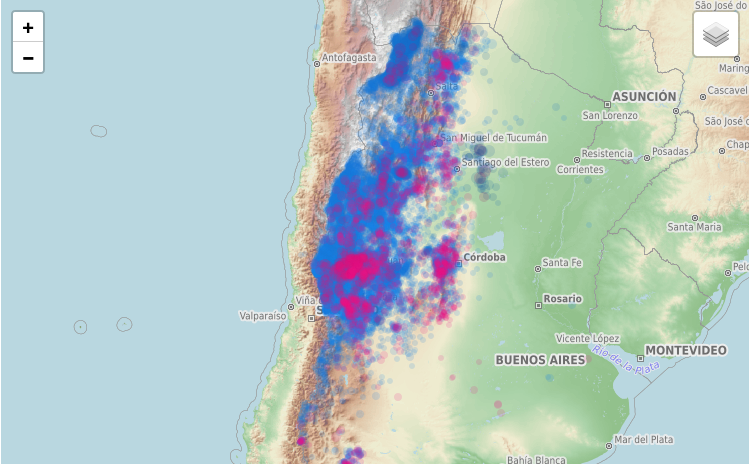
\includegraphics[width=0.8\textwidth]{mapa_sismos.png}
\caption{Superponer las ubicaciones de los terremotos en un mapa físico muestra que la mayoría de los terremotos se registran en zonas de montaña o cerros en su mayoría alejados de las mayores urbanizaciones, lo que afecta negativamente la estadística de los percibidos.
La escala de colores muestra los más superficiales en azul y profundos en rojo.
Reproducido de \cite{daniela_parada_ic-datasets-docencia_nodate}}
\label{fig:mapa_sismos}
\end{figure}

La ubicación de los terremotos sobre un mapa político que muestra la figura \ref{fig:terremotosMapa} deja a las claras que no tienen una distribución homogénea, aún en provincias con abundante actividad.

\begin{figure}[!ht]
\centering
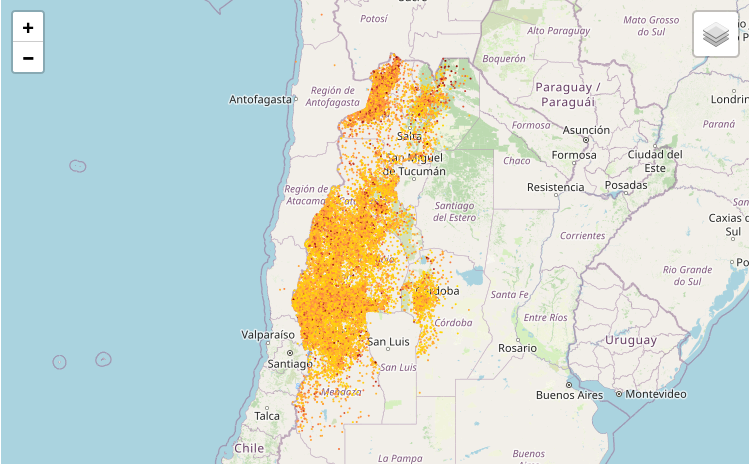
\includegraphics[width=0.8\textwidth]{terremotosMapa.png}
\caption{Sobre este mapa político se representan las ubicaciones de los terremotos como puntos. Esto permite apreciar que en algunas provincias, como San Luís, se omiten datas como evidencia el corte abrupto de reportes en su frontera. En otras se hacen más claros sesgos geográficos, como en Córdoba, Salta o Jujuy, 
Reproducido de \cite{daniela_parada_ic-datasets-docencia_nodate}}
\label{fig:terremotosMapa}
\end{figure}

% De lo observado en estas figuras se hace una selección del área geográfica de los datos a trabajar que se discute en la sección siguiente.


\paragraph{El problema de la distancia}
Evidentemente, la proximidad de un epicentro a una población es un factor relevante en la percepción de un sismo.
El INPRES tiene una metodología operativa para registrar la ubicación de los usuarios que reportan haber percibido un sismo a través de su página web \cite{noauthor_acerca_nodate}.
Su buscador de sismos indica los sismos ``sentidos'' por usuarios con un color en sus resultados de búsqueda como ilustra la figura \ref{fig:resultado_búsqueda}.

\begin{figure}[!ht]
\centering
\includegraphics[width=\textwidth]{resultado_búsqueda.png}
\caption{Resultados de una búsqueda manual de sismos en el sitio del INPRES. El indicado en rojo fue percibido por la población. En la columna \emph{intensidad} se dan datos de ubicación de la población que lo percibió, pero en una nomenclatura interna del INPRES que no pudo traducirse a una ubicación geográfica precisada por su latitud y longitud.}
\label{fig:resultado_búsqueda}
\end{figure}

Lamentablemente, en el conjunto de datos curados no figura la ubicación del sismógrafo o la población que hizo el registro lo que imposibilita incorporar la distancia al epicentro como una variable en el modelo.%sin realizar un nuevo \emph{scrapping} de estos datos en el sitio del INPRES.
Puesto que no se tiene control posible sobre la posición de quienes potencialmente percibieron un sismo se decidió para reducir el impacto del parámetro distancia limitar el espacio geográfico de los terremotos.
Las posibles fuentes de datos para realizar tal operación son su latitud, longitud y provincia.


\paragraph{Elección de la provincia de San Juan}
Respondiendo a la discutido en el párrafo anterior se buscó trabajar en un extensión geográfica relativamente limitada, pero cuidando que el número de sismos restantes sea aún elevado.
Tras una inspección visual de la figura \ref{fig:terremotosMapa} se determinó  que la provincia de San Juan cumple con tales requisitos, por lo que se procedió a filtrar los datos con el comando \lstinline[language = R]'sismos_SJ <- sismos[Provincia == "San Juan"]'.
El subconjunto de datos de esta provincia representa aproximadamente un \(54 \%\) de los datos hasta aquí disponibles.
Con \num{29917} registros es aún un número suficiente para realizar análisis cono los métodos elegidos.

% Se eligió entonces la provincia de San Juan por presentar un elevado número de casos percibidos o no en el conjunto de datos, por tener una extensión geográfica reducida en comparación con otras así como contar con una alta homogeneidad espacial en el reporte de sismos hace que el factor distancia entre epicentro y población que reporta tenga menor impacto que en otras provincias.


\paragraph{Latitud y longitud}
La distribución de terremotos en la provincia de San Juan dista de ser homogénea pues hay una preponderancia de las ubicaciones meridionales como puede apreciarse en la figura \ref{fig:sanJuan}.

\begin{figure}[!ht]
	\centering
	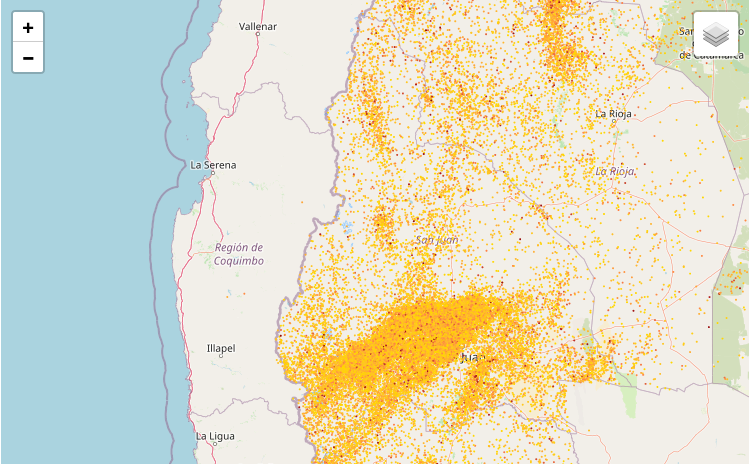
\includegraphics[width=0.8\textwidth]{sanJuan.png}
	\caption{Recorte de la figura \ref{fig:terremotosMapa} en torno a la provincia de San Juan.
	Los terremotos se presentan mayoritariamente en su región meridional.
	Los puntos rojos son los percibidos por personas.
	Reproducido de \cite{daniela_parada_ic-datasets-docencia_nodate}}
\label{fig:sanJuan}
\end{figure}

Lo anterior podría hacer sospechar de un sesgo con la latitud, pero la inspección visual de la figura muestra que la proporción de puntos rojos y amarillos, los de terremotos percibidos o no es similar con la que hay en el norte.
En función de esto se decidió no eliminar las variable de latitud en este estadio y analizar más adelante su correlación con la percepción de los sismos.
A fin de cuentas el objetivo del trabajo es determinar si un modelo puede predecir la percepción de un sismo por parte de la población y no determinar los factores que influyen en la percepción de los sismos por parte de la población.
En caso de que haya factores geográficos regionales, estos serán capturados por el modelo de clasificación y no necesariamente por la variable de latitud.

Un razonamiento similar se aplica para no coartar la variable de longitud.
Como se comentó al presentar la figura \ref{fig:mapa_sismos}, son esperables más terremotos y de mayor intensidad en las regiones occidentales de la provincia de San Juan.
Nuevamente será una virtud de los modelos si pueden explotar tal información para mejorar la clasificación de los sismos percibidos por la población.

% y que el reporte de sismos percibidos  no tenga sesgos geográficos, es decir una mayor preponderancia en regiones meridionales y/o orientales que en los sentidos opuestos.

%Por tal razón para este trabajo se obvian las variables de latitud y longitud del epicentro.
%Para que esto no sea una factor de sesgo en el modelo se decidió filtrar por la variable ``Provincia'' y trabajar con un subconjunto de los datos que correspondan a una provincia en particular.





\section{Análisis exploratorio de datos}\label{sec:AED}

Un primer vistazo sobre los datos con \lstinline[language = R]'summary(sismos_SJ)' permitió obtener un resumen de las variables numéricas y categóricas.
Saltan a la vista que hay valores extremos en el extremo superior de la variable \lstinline[language = R]'Magnitud' bastante alejados de la mediana y que hay un fuerte desequilibrio en la variable ``Percibido'', la de clase de clasificación, en favor de los terremotos no percibidos.


\paragraph{Desequilibrio en la clase de clasificación}
Sobre el total de registros solo un valor cercano al \(98\%\) fueron percibidos por el instrumental y no por la población.
Restan tan solo unos \num{619} registros que efectivamente fueron percibidos por la población.
Este desequilibrio llama al uso de técnicas de balanceo de clases en los modelos de clasificación a utilizar.


\paragraph{Distribución de la magnitud}
La magnitud de terremotos forzosamente presenta una distribución asimétrica por el hecho de que cuanto mayor es la energía liberada, más infrecuente es el fenómeno.
La relación logarítmica de la frecuencia con la magnitud de los sismos que muestra la figura \ref{fig:acumulado_anual_magnitud} para San Juan en los años 2012 a 2022 es universal es coincidente con lo enunciado en la ley empírica de Gutenberg-Richter \cite[ec. 4.24]{fowler_solid_1990}.

\begin{figure}[!ht]
%% \begin{wrapfigure}[13]{r}{0.5\textwidth}
\centering
% Created by tikzDevice version 0.12.6 on 2024-07-04 02:45:07
% !TEX encoding = UTF-8 Unicode
\begin{tikzpicture}[x=1pt,y=1pt]
\definecolor{fillColor}{RGB}{255,255,255}
\path[use as bounding box,fill=fillColor,fill opacity=0.00] (0,0) rectangle (361.35,216.81);
\begin{scope}
\path[clip] (  0.00,  0.00) rectangle (361.35,216.81);
\definecolor{drawColor}{RGB}{255,255,255}
\definecolor{fillColor}{RGB}{255,255,255}

\path[draw=drawColor,line width= 0.6pt,line join=round,line cap=round,fill=fillColor] (  0.00,  0.00) rectangle (361.35,216.81);
\end{scope}
\begin{scope}
\path[clip] ( 27.31, 30.69) rectangle (296.30,211.31);
\definecolor{fillColor}{RGB}{255,255,255}

\path[fill=fillColor] ( 27.31, 30.69) rectangle (296.30,211.31);
\definecolor{drawColor}{RGB}{248,118,109}
\definecolor{fillColor}{RGB}{248,118,109}

\path[draw=drawColor,line width= 0.4pt,line join=round,line cap=round,fill=fillColor] (208.83, 38.90) circle (  1.96);

\path[draw=drawColor,line width= 0.4pt,line join=round,line cap=round,fill=fillColor] (202.56, 52.59) circle (  1.96);

\path[draw=drawColor,line width= 0.4pt,line join=round,line cap=round,fill=fillColor] (183.75, 60.60) circle (  1.96);

\path[draw=drawColor,line width= 0.4pt,line join=round,line cap=round,fill=fillColor] (177.48, 70.69) circle (  1.96);

\path[draw=drawColor,line width= 0.4pt,line join=round,line cap=round,fill=fillColor] (171.21, 86.27) circle (  1.96);

\path[draw=drawColor,line width= 0.4pt,line join=round,line cap=round,fill=fillColor] (164.94, 94.87) circle (  1.96);

\path[draw=drawColor,line width= 0.4pt,line join=round,line cap=round,fill=fillColor] (158.67,100.84) circle (  1.96);

\path[draw=drawColor,line width= 0.4pt,line join=round,line cap=round,fill=fillColor] (152.40,106.74) circle (  1.96);

\path[draw=drawColor,line width= 0.4pt,line join=round,line cap=round,fill=fillColor] (146.13,112.74) circle (  1.96);

\path[draw=drawColor,line width= 0.4pt,line join=round,line cap=round,fill=fillColor] (139.86,118.77) circle (  1.96);

\path[draw=drawColor,line width= 0.4pt,line join=round,line cap=round,fill=fillColor] (133.59,125.47) circle (  1.96);

\path[draw=drawColor,line width= 0.4pt,line join=round,line cap=round,fill=fillColor] (127.32,129.48) circle (  1.96);

\path[draw=drawColor,line width= 0.4pt,line join=round,line cap=round,fill=fillColor] (121.05,135.21) circle (  1.96);

\path[draw=drawColor,line width= 0.4pt,line join=round,line cap=round,fill=fillColor] (114.78,140.12) circle (  1.96);

\path[draw=drawColor,line width= 0.4pt,line join=round,line cap=round,fill=fillColor] (108.51,145.72) circle (  1.96);

\path[draw=drawColor,line width= 0.4pt,line join=round,line cap=round,fill=fillColor] (102.24,151.91) circle (  1.96);

\path[draw=drawColor,line width= 0.4pt,line join=round,line cap=round,fill=fillColor] ( 95.97,157.21) circle (  1.96);

\path[draw=drawColor,line width= 0.4pt,line join=round,line cap=round,fill=fillColor] ( 89.70,162.71) circle (  1.96);

\path[draw=drawColor,line width= 0.4pt,line join=round,line cap=round,fill=fillColor] ( 83.43,168.29) circle (  1.96);

\path[draw=drawColor,line width= 0.4pt,line join=round,line cap=round,fill=fillColor] ( 77.16,173.44) circle (  1.96);

\path[draw=drawColor,line width= 0.4pt,line join=round,line cap=round,fill=fillColor] ( 70.89,177.99) circle (  1.96);

\path[draw=drawColor,line width= 0.4pt,line join=round,line cap=round,fill=fillColor] ( 64.62,182.85) circle (  1.96);

\path[draw=drawColor,line width= 0.4pt,line join=round,line cap=round,fill=fillColor] ( 58.35,186.71) circle (  1.96);

\path[draw=drawColor,line width= 0.4pt,line join=round,line cap=round,fill=fillColor] ( 52.08,190.36) circle (  1.96);

\path[draw=drawColor,line width= 0.4pt,line join=round,line cap=round,fill=fillColor] ( 45.81,193.56) circle (  1.96);

\path[draw=drawColor,line width= 0.4pt,line join=round,line cap=round,fill=fillColor] ( 39.54,196.26) circle (  1.96);
\definecolor{drawColor}{RGB}{219,142,0}
\definecolor{fillColor}{RGB}{219,142,0}

\path[draw=drawColor,line width= 0.4pt,line join=round,line cap=round,fill=fillColor] (221.37, 38.90) circle (  1.96);

\path[draw=drawColor,line width= 0.4pt,line join=round,line cap=round,fill=fillColor] (215.10, 52.59) circle (  1.96);

\path[draw=drawColor,line width= 0.4pt,line join=round,line cap=round,fill=fillColor] (202.56, 60.60) circle (  1.96);

\path[draw=drawColor,line width= 0.4pt,line join=round,line cap=round,fill=fillColor] (196.29, 70.69) circle (  1.96);

\path[draw=drawColor,line width= 0.4pt,line join=round,line cap=round,fill=fillColor] (190.02, 77.34) circle (  1.96);

\path[draw=drawColor,line width= 0.4pt,line join=round,line cap=round,fill=fillColor] (183.75, 84.39) circle (  1.96);

\path[draw=drawColor,line width= 0.4pt,line join=round,line cap=round,fill=fillColor] (177.48, 87.99) circle (  1.96);

\path[draw=drawColor,line width= 0.4pt,line join=round,line cap=round,fill=fillColor] (171.21, 89.57) circle (  1.96);

\path[draw=drawColor,line width= 0.4pt,line join=round,line cap=round,fill=fillColor] (164.94, 93.67) circle (  1.96);

\path[draw=drawColor,line width= 0.4pt,line join=round,line cap=round,fill=fillColor] (158.67, 98.08) circle (  1.96);

\path[draw=drawColor,line width= 0.4pt,line join=round,line cap=round,fill=fillColor] (152.40,105.42) circle (  1.96);

\path[draw=drawColor,line width= 0.4pt,line join=round,line cap=round,fill=fillColor] (146.13,110.23) circle (  1.96);

\path[draw=drawColor,line width= 0.4pt,line join=round,line cap=round,fill=fillColor] (139.86,115.37) circle (  1.96);

\path[draw=drawColor,line width= 0.4pt,line join=round,line cap=round,fill=fillColor] (133.59,119.78) circle (  1.96);

\path[draw=drawColor,line width= 0.4pt,line join=round,line cap=round,fill=fillColor] (127.32,122.83) circle (  1.96);

\path[draw=drawColor,line width= 0.4pt,line join=round,line cap=round,fill=fillColor] (121.05,129.68) circle (  1.96);

\path[draw=drawColor,line width= 0.4pt,line join=round,line cap=round,fill=fillColor] (114.78,134.75) circle (  1.96);

\path[draw=drawColor,line width= 0.4pt,line join=round,line cap=round,fill=fillColor] (108.51,141.81) circle (  1.96);

\path[draw=drawColor,line width= 0.4pt,line join=round,line cap=round,fill=fillColor] (102.24,147.42) circle (  1.96);

\path[draw=drawColor,line width= 0.4pt,line join=round,line cap=round,fill=fillColor] ( 95.97,152.98) circle (  1.96);

\path[draw=drawColor,line width= 0.4pt,line join=round,line cap=round,fill=fillColor] ( 89.70,158.13) circle (  1.96);

\path[draw=drawColor,line width= 0.4pt,line join=round,line cap=round,fill=fillColor] ( 83.43,163.80) circle (  1.96);

\path[draw=drawColor,line width= 0.4pt,line join=round,line cap=round,fill=fillColor] ( 77.16,169.09) circle (  1.96);

\path[draw=drawColor,line width= 0.4pt,line join=round,line cap=round,fill=fillColor] ( 70.89,174.33) circle (  1.96);

\path[draw=drawColor,line width= 0.4pt,line join=round,line cap=round,fill=fillColor] ( 64.62,178.38) circle (  1.96);

\path[draw=drawColor,line width= 0.4pt,line join=round,line cap=round,fill=fillColor] ( 58.35,182.42) circle (  1.96);

\path[draw=drawColor,line width= 0.4pt,line join=round,line cap=round,fill=fillColor] ( 52.08,186.48) circle (  1.96);

\path[draw=drawColor,line width= 0.4pt,line join=round,line cap=round,fill=fillColor] ( 45.81,189.73) circle (  1.96);

\path[draw=drawColor,line width= 0.4pt,line join=round,line cap=round,fill=fillColor] ( 39.54,192.64) circle (  1.96);
\definecolor{drawColor}{RGB}{174,162,0}
\definecolor{fillColor}{RGB}{174,162,0}

\path[draw=drawColor,line width= 0.4pt,line join=round,line cap=round,fill=fillColor] (233.91, 38.90) circle (  1.96);

\path[draw=drawColor,line width= 0.4pt,line join=round,line cap=round,fill=fillColor] (215.10, 52.59) circle (  1.96);

\path[draw=drawColor,line width= 0.4pt,line join=round,line cap=round,fill=fillColor] (196.29, 60.60) circle (  1.96);

\path[draw=drawColor,line width= 0.4pt,line join=round,line cap=round,fill=fillColor] (183.75, 70.69) circle (  1.96);

\path[draw=drawColor,line width= 0.4pt,line join=round,line cap=round,fill=fillColor] (177.48, 77.34) circle (  1.96);

\path[draw=drawColor,line width= 0.4pt,line join=round,line cap=round,fill=fillColor] (171.21, 82.30) circle (  1.96);

\path[draw=drawColor,line width= 0.4pt,line join=round,line cap=round,fill=fillColor] (158.67, 86.27) circle (  1.96);

\path[draw=drawColor,line width= 0.4pt,line join=round,line cap=round,fill=fillColor] (152.40, 93.67) circle (  1.96);

\path[draw=drawColor,line width= 0.4pt,line join=round,line cap=round,fill=fillColor] (146.13,101.68) circle (  1.96);

\path[draw=drawColor,line width= 0.4pt,line join=round,line cap=round,fill=fillColor] (139.86,108.56) circle (  1.96);

\path[draw=drawColor,line width= 0.4pt,line join=round,line cap=round,fill=fillColor] (133.59,114.10) circle (  1.96);

\path[draw=drawColor,line width= 0.4pt,line join=round,line cap=round,fill=fillColor] (127.32,118.06) circle (  1.96);

\path[draw=drawColor,line width= 0.4pt,line join=round,line cap=round,fill=fillColor] (121.05,123.39) circle (  1.96);

\path[draw=drawColor,line width= 0.4pt,line join=round,line cap=round,fill=fillColor] (114.78,129.68) circle (  1.96);

\path[draw=drawColor,line width= 0.4pt,line join=round,line cap=round,fill=fillColor] (108.51,134.28) circle (  1.96);

\path[draw=drawColor,line width= 0.4pt,line join=round,line cap=round,fill=fillColor] (102.24,140.70) circle (  1.96);

\path[draw=drawColor,line width= 0.4pt,line join=round,line cap=round,fill=fillColor] ( 95.97,146.16) circle (  1.96);

\path[draw=drawColor,line width= 0.4pt,line join=round,line cap=round,fill=fillColor] ( 89.70,152.48) circle (  1.96);

\path[draw=drawColor,line width= 0.4pt,line join=round,line cap=round,fill=fillColor] ( 83.43,157.89) circle (  1.96);

\path[draw=drawColor,line width= 0.4pt,line join=round,line cap=round,fill=fillColor] ( 77.16,163.66) circle (  1.96);

\path[draw=drawColor,line width= 0.4pt,line join=round,line cap=round,fill=fillColor] ( 70.89,169.84) circle (  1.96);

\path[draw=drawColor,line width= 0.4pt,line join=round,line cap=round,fill=fillColor] ( 64.62,175.72) circle (  1.96);

\path[draw=drawColor,line width= 0.4pt,line join=round,line cap=round,fill=fillColor] ( 58.35,181.25) circle (  1.96);

\path[draw=drawColor,line width= 0.4pt,line join=round,line cap=round,fill=fillColor] ( 52.08,186.57) circle (  1.96);

\path[draw=drawColor,line width= 0.4pt,line join=round,line cap=round,fill=fillColor] ( 45.81,191.46) circle (  1.96);

\path[draw=drawColor,line width= 0.4pt,line join=round,line cap=round,fill=fillColor] ( 39.54,195.63) circle (  1.96);
\definecolor{drawColor}{RGB}{100,178,0}
\definecolor{fillColor}{RGB}{100,178,0}

\path[draw=drawColor,line width= 0.4pt,line join=round,line cap=round,fill=fillColor] (183.75, 38.90) circle (  1.96);

\path[draw=drawColor,line width= 0.4pt,line join=round,line cap=round,fill=fillColor] (177.48, 60.60) circle (  1.96);

\path[draw=drawColor,line width= 0.4pt,line join=round,line cap=round,fill=fillColor] (171.21, 74.29) circle (  1.96);

\path[draw=drawColor,line width= 0.4pt,line join=round,line cap=round,fill=fillColor] (164.94, 82.30) circle (  1.96);

\path[draw=drawColor,line width= 0.4pt,line join=round,line cap=round,fill=fillColor] (158.67, 87.99) circle (  1.96);

\path[draw=drawColor,line width= 0.4pt,line join=round,line cap=round,fill=fillColor] (152.40, 89.57) circle (  1.96);

\path[draw=drawColor,line width= 0.4pt,line join=round,line cap=round,fill=fillColor] (146.13, 93.67) circle (  1.96);

\path[draw=drawColor,line width= 0.4pt,line join=round,line cap=round,fill=fillColor] (139.86, 99.04) circle (  1.96);

\path[draw=drawColor,line width= 0.4pt,line join=round,line cap=round,fill=fillColor] (133.59,101.68) circle (  1.96);

\path[draw=drawColor,line width= 0.4pt,line join=round,line cap=round,fill=fillColor] (127.32,109.69) circle (  1.96);

\path[draw=drawColor,line width= 0.4pt,line join=round,line cap=round,fill=fillColor] (121.05,115.37) circle (  1.96);

\path[draw=drawColor,line width= 0.4pt,line join=round,line cap=round,fill=fillColor] (114.78,120.43) circle (  1.96);

\path[draw=drawColor,line width= 0.4pt,line join=round,line cap=round,fill=fillColor] (108.51,126.19) circle (  1.96);

\path[draw=drawColor,line width= 0.4pt,line join=round,line cap=round,fill=fillColor] (102.24,131.76) circle (  1.96);

\path[draw=drawColor,line width= 0.4pt,line join=round,line cap=round,fill=fillColor] ( 95.97,137.08) circle (  1.96);

\path[draw=drawColor,line width= 0.4pt,line join=round,line cap=round,fill=fillColor] ( 89.70,143.67) circle (  1.96);

\path[draw=drawColor,line width= 0.4pt,line join=round,line cap=round,fill=fillColor] ( 83.43,150.70) circle (  1.96);

\path[draw=drawColor,line width= 0.4pt,line join=round,line cap=round,fill=fillColor] ( 77.16,157.31) circle (  1.96);

\path[draw=drawColor,line width= 0.4pt,line join=round,line cap=round,fill=fillColor] ( 70.89,163.70) circle (  1.96);

\path[draw=drawColor,line width= 0.4pt,line join=round,line cap=round,fill=fillColor] ( 64.62,169.09) circle (  1.96);

\path[draw=drawColor,line width= 0.4pt,line join=round,line cap=round,fill=fillColor] ( 58.35,175.40) circle (  1.96);

\path[draw=drawColor,line width= 0.4pt,line join=round,line cap=round,fill=fillColor] ( 52.08,181.01) circle (  1.96);

\path[draw=drawColor,line width= 0.4pt,line join=round,line cap=round,fill=fillColor] ( 45.81,186.17) circle (  1.96);

\path[draw=drawColor,line width= 0.4pt,line join=round,line cap=round,fill=fillColor] ( 39.54,191.27) circle (  1.96);
\definecolor{drawColor}{RGB}{0,189,92}
\definecolor{fillColor}{RGB}{0,189,92}

\path[draw=drawColor,line width= 0.4pt,line join=round,line cap=round,fill=fillColor] (277.80, 38.90) circle (  1.96);

\path[draw=drawColor,line width= 0.4pt,line join=round,line cap=round,fill=fillColor] (202.56, 60.60) circle (  1.96);

\path[draw=drawColor,line width= 0.4pt,line join=round,line cap=round,fill=fillColor] (190.02, 66.28) circle (  1.96);

\path[draw=drawColor,line width= 0.4pt,line join=round,line cap=round,fill=fillColor] (183.75, 70.69) circle (  1.96);

\path[draw=drawColor,line width= 0.4pt,line join=round,line cap=round,fill=fillColor] (177.48, 74.29) circle (  1.96);

\path[draw=drawColor,line width= 0.4pt,line join=round,line cap=round,fill=fillColor] (171.21, 79.98) circle (  1.96);

\path[draw=drawColor,line width= 0.4pt,line join=round,line cap=round,fill=fillColor] (164.94, 86.27) circle (  1.96);

\path[draw=drawColor,line width= 0.4pt,line join=round,line cap=round,fill=fillColor] (158.67, 93.67) circle (  1.96);

\path[draw=drawColor,line width= 0.4pt,line join=round,line cap=round,fill=fillColor] (152.40, 97.07) circle (  1.96);

\path[draw=drawColor,line width= 0.4pt,line join=round,line cap=round,fill=fillColor] (146.13, 99.96) circle (  1.96);

\path[draw=drawColor,line width= 0.4pt,line join=round,line cap=round,fill=fillColor] (139.86,104.01) circle (  1.96);

\path[draw=drawColor,line width= 0.4pt,line join=round,line cap=round,fill=fillColor] (133.59,107.36) circle (  1.96);

\path[draw=drawColor,line width= 0.4pt,line join=round,line cap=round,fill=fillColor] (127.32,111.77) circle (  1.96);

\path[draw=drawColor,line width= 0.4pt,line join=round,line cap=round,fill=fillColor] (121.05,115.37) circle (  1.96);

\path[draw=drawColor,line width= 0.4pt,line join=round,line cap=round,fill=fillColor] (114.78,119.45) circle (  1.96);

\path[draw=drawColor,line width= 0.4pt,line join=round,line cap=round,fill=fillColor] (108.51,124.19) circle (  1.96);

\path[draw=drawColor,line width= 0.4pt,line join=round,line cap=round,fill=fillColor] (102.24,129.48) circle (  1.96);

\path[draw=drawColor,line width= 0.4pt,line join=round,line cap=round,fill=fillColor] ( 95.97,135.36) circle (  1.96);

\path[draw=drawColor,line width= 0.4pt,line join=round,line cap=round,fill=fillColor] ( 89.70,141.49) circle (  1.96);

\path[draw=drawColor,line width= 0.4pt,line join=round,line cap=round,fill=fillColor] ( 83.43,148.83) circle (  1.96);

\path[draw=drawColor,line width= 0.4pt,line join=round,line cap=round,fill=fillColor] ( 77.16,156.30) circle (  1.96);

\path[draw=drawColor,line width= 0.4pt,line join=round,line cap=round,fill=fillColor] ( 70.89,163.26) circle (  1.96);

\path[draw=drawColor,line width= 0.4pt,line join=round,line cap=round,fill=fillColor] ( 64.62,169.65) circle (  1.96);

\path[draw=drawColor,line width= 0.4pt,line join=round,line cap=round,fill=fillColor] ( 58.35,175.79) circle (  1.96);

\path[draw=drawColor,line width= 0.4pt,line join=round,line cap=round,fill=fillColor] ( 52.08,181.70) circle (  1.96);

\path[draw=drawColor,line width= 0.4pt,line join=round,line cap=round,fill=fillColor] ( 45.81,186.81) circle (  1.96);

\path[draw=drawColor,line width= 0.4pt,line join=round,line cap=round,fill=fillColor] ( 39.54,192.01) circle (  1.96);
\definecolor{drawColor}{RGB}{0,193,167}
\definecolor{fillColor}{RGB}{0,193,167}

\path[draw=drawColor,line width= 0.4pt,line join=round,line cap=round,fill=fillColor] (215.10, 38.90) circle (  1.96);

\path[draw=drawColor,line width= 0.4pt,line join=round,line cap=round,fill=fillColor] (177.48, 60.60) circle (  1.96);

\path[draw=drawColor,line width= 0.4pt,line join=round,line cap=round,fill=fillColor] (171.21, 66.28) circle (  1.96);

\path[draw=drawColor,line width= 0.4pt,line join=round,line cap=round,fill=fillColor] (164.94, 70.69) circle (  1.96);

\path[draw=drawColor,line width= 0.4pt,line join=round,line cap=round,fill=fillColor] (158.67, 77.34) circle (  1.96);

\path[draw=drawColor,line width= 0.4pt,line join=round,line cap=round,fill=fillColor] (152.40, 87.99) circle (  1.96);

\path[draw=drawColor,line width= 0.4pt,line join=round,line cap=round,fill=fillColor] (146.13, 93.67) circle (  1.96);

\path[draw=drawColor,line width= 0.4pt,line join=round,line cap=round,fill=fillColor] (139.86, 98.08) circle (  1.96);

\path[draw=drawColor,line width= 0.4pt,line join=round,line cap=round,fill=fillColor] (133.59,104.01) circle (  1.96);

\path[draw=drawColor,line width= 0.4pt,line join=round,line cap=round,fill=fillColor] (127.32,110.23) circle (  1.96);

\path[draw=drawColor,line width= 0.4pt,line join=round,line cap=round,fill=fillColor] (121.05,113.20) circle (  1.96);

\path[draw=drawColor,line width= 0.4pt,line join=round,line cap=round,fill=fillColor] (114.78,122.26) circle (  1.96);

\path[draw=drawColor,line width= 0.4pt,line join=round,line cap=round,fill=fillColor] (108.51,127.79) circle (  1.96);

\path[draw=drawColor,line width= 0.4pt,line join=round,line cap=round,fill=fillColor] (102.24,131.58) circle (  1.96);

\path[draw=drawColor,line width= 0.4pt,line join=round,line cap=round,fill=fillColor] ( 95.97,139.04) circle (  1.96);

\path[draw=drawColor,line width= 0.4pt,line join=round,line cap=round,fill=fillColor] ( 89.70,145.63) circle (  1.96);

\path[draw=drawColor,line width= 0.4pt,line join=round,line cap=round,fill=fillColor] ( 83.43,152.98) circle (  1.96);

\path[draw=drawColor,line width= 0.4pt,line join=round,line cap=round,fill=fillColor] ( 77.16,158.87) circle (  1.96);

\path[draw=drawColor,line width= 0.4pt,line join=round,line cap=round,fill=fillColor] ( 70.89,164.67) circle (  1.96);

\path[draw=drawColor,line width= 0.4pt,line join=round,line cap=round,fill=fillColor] ( 64.62,171.49) circle (  1.96);

\path[draw=drawColor,line width= 0.4pt,line join=round,line cap=round,fill=fillColor] ( 58.35,177.43) circle (  1.96);

\path[draw=drawColor,line width= 0.4pt,line join=round,line cap=round,fill=fillColor] ( 52.08,182.95) circle (  1.96);

\path[draw=drawColor,line width= 0.4pt,line join=round,line cap=round,fill=fillColor] ( 45.81,187.55) circle (  1.96);

\path[draw=drawColor,line width= 0.4pt,line join=round,line cap=round,fill=fillColor] ( 39.54,191.39) circle (  1.96);
\definecolor{drawColor}{RGB}{0,186,222}
\definecolor{fillColor}{RGB}{0,186,222}

\path[draw=drawColor,line width= 0.4pt,line join=round,line cap=round,fill=fillColor] (221.37, 52.59) circle (  1.96);

\path[draw=drawColor,line width= 0.4pt,line join=round,line cap=round,fill=fillColor] (202.56, 66.28) circle (  1.96);

\path[draw=drawColor,line width= 0.4pt,line join=round,line cap=round,fill=fillColor] (183.75, 70.69) circle (  1.96);

\path[draw=drawColor,line width= 0.4pt,line join=round,line cap=round,fill=fillColor] (177.48, 74.29) circle (  1.96);

\path[draw=drawColor,line width= 0.4pt,line join=round,line cap=round,fill=fillColor] (171.21, 79.98) circle (  1.96);

\path[draw=drawColor,line width= 0.4pt,line join=round,line cap=round,fill=fillColor] (158.67, 86.27) circle (  1.96);

\path[draw=drawColor,line width= 0.4pt,line join=round,line cap=round,fill=fillColor] (146.13, 91.03) circle (  1.96);

\path[draw=drawColor,line width= 0.4pt,line join=round,line cap=round,fill=fillColor] (139.86,100.84) circle (  1.96);

\path[draw=drawColor,line width= 0.4pt,line join=round,line cap=round,fill=fillColor] (133.59,104.01) circle (  1.96);

\path[draw=drawColor,line width= 0.4pt,line join=round,line cap=round,fill=fillColor] (127.32,106.09) circle (  1.96);

\path[draw=drawColor,line width= 0.4pt,line join=round,line cap=round,fill=fillColor] (121.05,110.76) circle (  1.96);

\path[draw=drawColor,line width= 0.4pt,line join=round,line cap=round,fill=fillColor] (114.78,119.45) circle (  1.96);

\path[draw=drawColor,line width= 0.4pt,line join=round,line cap=round,fill=fillColor] (108.51,125.22) circle (  1.96);

\path[draw=drawColor,line width= 0.4pt,line join=round,line cap=round,fill=fillColor] (102.24,130.84) circle (  1.96);

\path[draw=drawColor,line width= 0.4pt,line join=round,line cap=round,fill=fillColor] ( 95.97,137.75) circle (  1.96);

\path[draw=drawColor,line width= 0.4pt,line join=round,line cap=round,fill=fillColor] ( 89.70,144.53) circle (  1.96);

\path[draw=drawColor,line width= 0.4pt,line join=round,line cap=round,fill=fillColor] ( 83.43,150.00) circle (  1.96);

\path[draw=drawColor,line width= 0.4pt,line join=round,line cap=round,fill=fillColor] ( 77.16,156.51) circle (  1.96);

\path[draw=drawColor,line width= 0.4pt,line join=round,line cap=round,fill=fillColor] ( 70.89,164.16) circle (  1.96);

\path[draw=drawColor,line width= 0.4pt,line join=round,line cap=round,fill=fillColor] ( 64.62,171.20) circle (  1.96);

\path[draw=drawColor,line width= 0.4pt,line join=round,line cap=round,fill=fillColor] ( 58.35,178.42) circle (  1.96);

\path[draw=drawColor,line width= 0.4pt,line join=round,line cap=round,fill=fillColor] ( 52.08,185.57) circle (  1.96);

\path[draw=drawColor,line width= 0.4pt,line join=round,line cap=round,fill=fillColor] ( 45.81,191.99) circle (  1.96);

\path[draw=drawColor,line width= 0.4pt,line join=round,line cap=round,fill=fillColor] ( 39.54,197.45) circle (  1.96);
\definecolor{drawColor}{RGB}{0,166,255}
\definecolor{fillColor}{RGB}{0,166,255}

\path[draw=drawColor,line width= 0.4pt,line join=round,line cap=round,fill=fillColor] (233.91, 38.90) circle (  1.96);

\path[draw=drawColor,line width= 0.4pt,line join=round,line cap=round,fill=fillColor] (215.10, 52.59) circle (  1.96);

\path[draw=drawColor,line width= 0.4pt,line join=round,line cap=round,fill=fillColor] (208.83, 60.60) circle (  1.96);

\path[draw=drawColor,line width= 0.4pt,line join=round,line cap=round,fill=fillColor] (190.02, 66.28) circle (  1.96);

\path[draw=drawColor,line width= 0.4pt,line join=round,line cap=round,fill=fillColor] (183.75, 74.29) circle (  1.96);

\path[draw=drawColor,line width= 0.4pt,line join=round,line cap=round,fill=fillColor] (164.94, 77.34) circle (  1.96);

\path[draw=drawColor,line width= 0.4pt,line join=round,line cap=round,fill=fillColor] (158.67, 79.98) circle (  1.96);

\path[draw=drawColor,line width= 0.4pt,line join=round,line cap=round,fill=fillColor] (152.40, 86.27) circle (  1.96);

\path[draw=drawColor,line width= 0.4pt,line join=round,line cap=round,fill=fillColor] (146.13, 94.87) circle (  1.96);

\path[draw=drawColor,line width= 0.4pt,line join=round,line cap=round,fill=fillColor] (139.86, 99.96) circle (  1.96);

\path[draw=drawColor,line width= 0.4pt,line join=round,line cap=round,fill=fillColor] (133.59,102.49) circle (  1.96);

\path[draw=drawColor,line width= 0.4pt,line join=round,line cap=round,fill=fillColor] (127.32,107.36) circle (  1.96);

\path[draw=drawColor,line width= 0.4pt,line join=round,line cap=round,fill=fillColor] (121.05,112.74) circle (  1.96);

\path[draw=drawColor,line width= 0.4pt,line join=round,line cap=round,fill=fillColor] (114.78,116.96) circle (  1.96);

\path[draw=drawColor,line width= 0.4pt,line join=round,line cap=round,fill=fillColor] (108.51,124.45) circle (  1.96);

\path[draw=drawColor,line width= 0.4pt,line join=round,line cap=round,fill=fillColor] (102.24,131.58) circle (  1.96);

\path[draw=drawColor,line width= 0.4pt,line join=round,line cap=round,fill=fillColor] ( 95.97,138.28) circle (  1.96);

\path[draw=drawColor,line width= 0.4pt,line join=round,line cap=round,fill=fillColor] ( 89.70,143.86) circle (  1.96);

\path[draw=drawColor,line width= 0.4pt,line join=round,line cap=round,fill=fillColor] ( 83.43,150.70) circle (  1.96);

\path[draw=drawColor,line width= 0.4pt,line join=round,line cap=round,fill=fillColor] ( 77.16,158.32) circle (  1.96);

\path[draw=drawColor,line width= 0.4pt,line join=round,line cap=round,fill=fillColor] ( 70.89,165.31) circle (  1.96);

\path[draw=drawColor,line width= 0.4pt,line join=round,line cap=round,fill=fillColor] ( 64.62,172.11) circle (  1.96);

\path[draw=drawColor,line width= 0.4pt,line join=round,line cap=round,fill=fillColor] ( 58.35,180.13) circle (  1.96);

\path[draw=drawColor,line width= 0.4pt,line join=round,line cap=round,fill=fillColor] ( 52.08,186.64) circle (  1.96);

\path[draw=drawColor,line width= 0.4pt,line join=round,line cap=round,fill=fillColor] ( 45.81,192.95) circle (  1.96);

\path[draw=drawColor,line width= 0.4pt,line join=round,line cap=round,fill=fillColor] ( 39.54,198.33) circle (  1.96);
\definecolor{drawColor}{RGB}{179,133,255}
\definecolor{fillColor}{RGB}{179,133,255}

\path[draw=drawColor,line width= 0.4pt,line join=round,line cap=round,fill=fillColor] (202.56, 38.90) circle (  1.96);

\path[draw=drawColor,line width= 0.4pt,line join=round,line cap=round,fill=fillColor] (190.02, 52.59) circle (  1.96);

\path[draw=drawColor,line width= 0.4pt,line join=round,line cap=round,fill=fillColor] (177.48, 66.28) circle (  1.96);

\path[draw=drawColor,line width= 0.4pt,line join=round,line cap=round,fill=fillColor] (171.21, 70.69) circle (  1.96);

\path[draw=drawColor,line width= 0.4pt,line join=round,line cap=round,fill=fillColor] (164.94, 77.34) circle (  1.96);

\path[draw=drawColor,line width= 0.4pt,line join=round,line cap=round,fill=fillColor] (158.67, 86.27) circle (  1.96);

\path[draw=drawColor,line width= 0.4pt,line join=round,line cap=round,fill=fillColor] (152.40, 94.87) circle (  1.96);

\path[draw=drawColor,line width= 0.4pt,line join=round,line cap=round,fill=fillColor] (146.13, 97.07) circle (  1.96);

\path[draw=drawColor,line width= 0.4pt,line join=round,line cap=round,fill=fillColor] (139.86, 99.96) circle (  1.96);

\path[draw=drawColor,line width= 0.4pt,line join=round,line cap=round,fill=fillColor] (133.59,107.36) circle (  1.96);

\path[draw=drawColor,line width= 0.4pt,line join=round,line cap=round,fill=fillColor] (127.32,113.66) circle (  1.96);

\path[draw=drawColor,line width= 0.4pt,line join=round,line cap=round,fill=fillColor] (121.05,117.70) circle (  1.96);

\path[draw=drawColor,line width= 0.4pt,line join=round,line cap=round,fill=fillColor] (114.78,122.26) circle (  1.96);

\path[draw=drawColor,line width= 0.4pt,line join=round,line cap=round,fill=fillColor] (108.51,126.43) circle (  1.96);

\path[draw=drawColor,line width= 0.4pt,line join=round,line cap=round,fill=fillColor] (102.24,131.94) circle (  1.96);

\path[draw=drawColor,line width= 0.4pt,line join=round,line cap=round,fill=fillColor] ( 95.97,137.89) circle (  1.96);

\path[draw=drawColor,line width= 0.4pt,line join=round,line cap=round,fill=fillColor] ( 89.70,145.81) circle (  1.96);

\path[draw=drawColor,line width= 0.4pt,line join=round,line cap=round,fill=fillColor] ( 83.43,152.73) circle (  1.96);

\path[draw=drawColor,line width= 0.4pt,line join=round,line cap=round,fill=fillColor] ( 77.16,159.98) circle (  1.96);

\path[draw=drawColor,line width= 0.4pt,line join=round,line cap=round,fill=fillColor] ( 70.89,166.14) circle (  1.96);

\path[draw=drawColor,line width= 0.4pt,line join=round,line cap=round,fill=fillColor] ( 64.62,173.74) circle (  1.96);

\path[draw=drawColor,line width= 0.4pt,line join=round,line cap=round,fill=fillColor] ( 58.35,180.53) circle (  1.96);

\path[draw=drawColor,line width= 0.4pt,line join=round,line cap=round,fill=fillColor] ( 52.08,187.50) circle (  1.96);

\path[draw=drawColor,line width= 0.4pt,line join=round,line cap=round,fill=fillColor] ( 45.81,193.47) circle (  1.96);

\path[draw=drawColor,line width= 0.4pt,line join=round,line cap=round,fill=fillColor] ( 39.54,198.93) circle (  1.96);
\definecolor{drawColor}{RGB}{239,103,235}
\definecolor{fillColor}{RGB}{239,103,235}

\path[draw=drawColor,line width= 0.4pt,line join=round,line cap=round,fill=fillColor] (284.07, 38.90) circle (  1.96);

\path[draw=drawColor,line width= 0.4pt,line join=round,line cap=round,fill=fillColor] (208.83, 52.59) circle (  1.96);

\path[draw=drawColor,line width= 0.4pt,line join=round,line cap=round,fill=fillColor] (202.56, 60.60) circle (  1.96);

\path[draw=drawColor,line width= 0.4pt,line join=round,line cap=round,fill=fillColor] (196.29, 66.28) circle (  1.96);

\path[draw=drawColor,line width= 0.4pt,line join=round,line cap=round,fill=fillColor] (190.02, 70.69) circle (  1.96);

\path[draw=drawColor,line width= 0.4pt,line join=round,line cap=round,fill=fillColor] (183.75, 77.34) circle (  1.96);

\path[draw=drawColor,line width= 0.4pt,line join=round,line cap=round,fill=fillColor] (177.48, 79.98) circle (  1.96);

\path[draw=drawColor,line width= 0.4pt,line join=round,line cap=round,fill=fillColor] (171.21, 84.39) circle (  1.96);

\path[draw=drawColor,line width= 0.4pt,line join=round,line cap=round,fill=fillColor] (164.94, 86.27) circle (  1.96);

\path[draw=drawColor,line width= 0.4pt,line join=round,line cap=round,fill=fillColor] (152.40, 89.57) circle (  1.96);

\path[draw=drawColor,line width= 0.4pt,line join=round,line cap=round,fill=fillColor] (146.13, 97.07) circle (  1.96);

\path[draw=drawColor,line width= 0.4pt,line join=round,line cap=round,fill=fillColor] (139.86, 99.04) circle (  1.96);

\path[draw=drawColor,line width= 0.4pt,line join=round,line cap=round,fill=fillColor] (133.59,105.42) circle (  1.96);

\path[draw=drawColor,line width= 0.4pt,line join=round,line cap=round,fill=fillColor] (127.32,111.27) circle (  1.96);

\path[draw=drawColor,line width= 0.4pt,line join=round,line cap=round,fill=fillColor] (121.05,119.11) circle (  1.96);

\path[draw=drawColor,line width= 0.4pt,line join=round,line cap=round,fill=fillColor] (114.78,122.54) circle (  1.96);

\path[draw=drawColor,line width= 0.4pt,line join=round,line cap=round,fill=fillColor] (108.51,126.90) circle (  1.96);

\path[draw=drawColor,line width= 0.4pt,line join=round,line cap=round,fill=fillColor] (102.24,135.21) circle (  1.96);

\path[draw=drawColor,line width= 0.4pt,line join=round,line cap=round,fill=fillColor] ( 95.97,142.56) circle (  1.96);

\path[draw=drawColor,line width= 0.4pt,line join=round,line cap=round,fill=fillColor] ( 89.70,149.28) circle (  1.96);

\path[draw=drawColor,line width= 0.4pt,line join=round,line cap=round,fill=fillColor] ( 83.43,156.86) circle (  1.96);

\path[draw=drawColor,line width= 0.4pt,line join=round,line cap=round,fill=fillColor] ( 77.16,164.05) circle (  1.96);

\path[draw=drawColor,line width= 0.4pt,line join=round,line cap=round,fill=fillColor] ( 70.89,170.96) circle (  1.96);

\path[draw=drawColor,line width= 0.4pt,line join=round,line cap=round,fill=fillColor] ( 64.62,178.80) circle (  1.96);

\path[draw=drawColor,line width= 0.4pt,line join=round,line cap=round,fill=fillColor] ( 58.35,185.64) circle (  1.96);

\path[draw=drawColor,line width= 0.4pt,line join=round,line cap=round,fill=fillColor] ( 52.08,192.00) circle (  1.96);

\path[draw=drawColor,line width= 0.4pt,line join=round,line cap=round,fill=fillColor] ( 45.81,198.08) circle (  1.96);

\path[draw=drawColor,line width= 0.4pt,line join=round,line cap=round,fill=fillColor] ( 39.54,203.10) circle (  1.96);
\definecolor{drawColor}{RGB}{255,99,182}
\definecolor{fillColor}{RGB}{255,99,182}

\path[draw=drawColor,line width= 0.4pt,line join=round,line cap=round,fill=fillColor] (208.83, 38.90) circle (  1.96);

\path[draw=drawColor,line width= 0.4pt,line join=round,line cap=round,fill=fillColor] (202.56, 52.59) circle (  1.96);

\path[draw=drawColor,line width= 0.4pt,line join=round,line cap=round,fill=fillColor] (171.21, 60.60) circle (  1.96);

\path[draw=drawColor,line width= 0.4pt,line join=round,line cap=round,fill=fillColor] (158.67, 66.28) circle (  1.96);

\path[draw=drawColor,line width= 0.4pt,line join=round,line cap=round,fill=fillColor] (139.86, 86.27) circle (  1.96);

\path[draw=drawColor,line width= 0.4pt,line join=round,line cap=round,fill=fillColor] (133.59, 89.57) circle (  1.96);

\path[draw=drawColor,line width= 0.4pt,line join=round,line cap=round,fill=fillColor] (127.32, 93.67) circle (  1.96);

\path[draw=drawColor,line width= 0.4pt,line join=round,line cap=round,fill=fillColor] (121.05,100.84) circle (  1.96);

\path[draw=drawColor,line width= 0.4pt,line join=round,line cap=round,fill=fillColor] (114.78,104.73) circle (  1.96);

\path[draw=drawColor,line width= 0.4pt,line join=round,line cap=round,fill=fillColor] (108.51,107.97) circle (  1.96);

\path[draw=drawColor,line width= 0.4pt,line join=round,line cap=round,fill=fillColor] (102.24,115.78) circle (  1.96);

\path[draw=drawColor,line width= 0.4pt,line join=round,line cap=round,fill=fillColor] ( 95.97,123.11) circle (  1.96);

\path[draw=drawColor,line width= 0.4pt,line join=round,line cap=round,fill=fillColor] ( 89.70,129.68) circle (  1.96);

\path[draw=drawColor,line width= 0.4pt,line join=round,line cap=round,fill=fillColor] ( 83.43,135.95) circle (  1.96);

\path[draw=drawColor,line width= 0.4pt,line join=round,line cap=round,fill=fillColor] ( 77.16,143.37) circle (  1.96);

\path[draw=drawColor,line width= 0.4pt,line join=round,line cap=round,fill=fillColor] ( 70.89,150.36) circle (  1.96);

\path[draw=drawColor,line width= 0.4pt,line join=round,line cap=round,fill=fillColor] ( 64.62,156.46) circle (  1.96);

\path[draw=drawColor,line width= 0.4pt,line join=round,line cap=round,fill=fillColor] ( 58.35,163.52) circle (  1.96);

\path[draw=drawColor,line width= 0.4pt,line join=round,line cap=round,fill=fillColor] ( 52.08,170.73) circle (  1.96);

\path[draw=drawColor,line width= 0.4pt,line join=round,line cap=round,fill=fillColor] ( 45.81,176.79) circle (  1.96);

\path[draw=drawColor,line width= 0.4pt,line join=round,line cap=round,fill=fillColor] ( 39.54,182.26) circle (  1.96);
\end{scope}
\begin{scope}
\path[clip] (  0.00,  0.00) rectangle (361.35,216.81);
\definecolor{drawColor}{RGB}{0,0,0}

\path[draw=drawColor,line width= 0.6pt,line join=round] ( 27.31, 30.69) --
	( 27.31,211.31);
\end{scope}
\begin{scope}
\path[clip] (  0.00,  0.00) rectangle (361.35,216.81);
\definecolor{drawColor}{gray}{0.30}

\node[text=drawColor,anchor=base east,inner sep=0pt, outer sep=0pt, scale=  0.88] at ( 22.36, 35.87) {0};

\node[text=drawColor,anchor=base east,inner sep=0pt, outer sep=0pt, scale=  0.88] at ( 22.36, 81.36) {1};

\node[text=drawColor,anchor=base east,inner sep=0pt, outer sep=0pt, scale=  0.88] at ( 22.36,126.84) {2};

\node[text=drawColor,anchor=base east,inner sep=0pt, outer sep=0pt, scale=  0.88] at ( 22.36,172.33) {3};
\end{scope}
\begin{scope}
\path[clip] (  0.00,  0.00) rectangle (361.35,216.81);
\definecolor{drawColor}{gray}{0.20}

\path[draw=drawColor,line width= 0.6pt,line join=round] ( 24.56, 38.90) --
	( 27.31, 38.90);

\path[draw=drawColor,line width= 0.6pt,line join=round] ( 24.56, 84.39) --
	( 27.31, 84.39);

\path[draw=drawColor,line width= 0.6pt,line join=round] ( 24.56,129.88) --
	( 27.31,129.88);

\path[draw=drawColor,line width= 0.6pt,line join=round] ( 24.56,175.36) --
	( 27.31,175.36);
\end{scope}
\begin{scope}
\path[clip] (  0.00,  0.00) rectangle (361.35,216.81);
\definecolor{drawColor}{RGB}{0,0,0}

\path[draw=drawColor,line width= 0.6pt,line join=round] ( 27.31, 30.69) --
	(296.30, 30.69);
\end{scope}
\begin{scope}
\path[clip] (  0.00,  0.00) rectangle (361.35,216.81);
\definecolor{drawColor}{gray}{0.20}

\path[draw=drawColor,line width= 0.6pt,line join=round] ( 70.89, 27.94) --
	( 70.89, 30.69);

\path[draw=drawColor,line width= 0.6pt,line join=round] (133.59, 27.94) --
	(133.59, 30.69);

\path[draw=drawColor,line width= 0.6pt,line join=round] (196.29, 27.94) --
	(196.29, 30.69);

\path[draw=drawColor,line width= 0.6pt,line join=round] (258.99, 27.94) --
	(258.99, 30.69);
\end{scope}
\begin{scope}
\path[clip] (  0.00,  0.00) rectangle (361.35,216.81);
\definecolor{drawColor}{gray}{0.30}

\node[text=drawColor,anchor=base,inner sep=0pt, outer sep=0pt, scale=  0.88] at ( 70.89, 19.68) {3};

\node[text=drawColor,anchor=base,inner sep=0pt, outer sep=0pt, scale=  0.88] at (133.59, 19.68) {4};

\node[text=drawColor,anchor=base,inner sep=0pt, outer sep=0pt, scale=  0.88] at (196.29, 19.68) {5};

\node[text=drawColor,anchor=base,inner sep=0pt, outer sep=0pt, scale=  0.88] at (258.99, 19.68) {6};
\end{scope}
\begin{scope}
\path[clip] (  0.00,  0.00) rectangle (361.35,216.81);
\definecolor{drawColor}{RGB}{0,0,0}

\node[text=drawColor,anchor=base,inner sep=0pt, outer sep=0pt, scale=  1.10] at (161.81,  7.64) {Magnitud ($M_w$)};
\end{scope}
\begin{scope}
\path[clip] (  0.00,  0.00) rectangle (361.35,216.81);
\definecolor{drawColor}{RGB}{0,0,0}

\node[text=drawColor,rotate= 90.00,anchor=base,inner sep=0pt, outer sep=0pt, scale=  1.10] at ( 13.08,121.00) {Número sismos (Log$_{10}$)};
\end{scope}
\begin{scope}
\path[clip] (  0.00,  0.00) rectangle (361.35,216.81);
\definecolor{fillColor}{RGB}{255,255,255}

\path[fill=fillColor] (307.30, 28.39) rectangle (355.85,213.60);
\end{scope}
\begin{scope}
\path[clip] (  0.00,  0.00) rectangle (361.35,216.81);
\definecolor{drawColor}{RGB}{0,0,0}

\node[text=drawColor,anchor=base west,inner sep=0pt, outer sep=0pt, scale=  1.10] at (312.80,199.46) {Año};
\end{scope}
\begin{scope}
\path[clip] (  0.00,  0.00) rectangle (361.35,216.81);
\definecolor{drawColor}{RGB}{248,118,109}
\definecolor{fillColor}{RGB}{248,118,109}

\path[draw=drawColor,line width= 0.4pt,line join=round,line cap=round,fill=fillColor] (320.03,185.66) circle (  1.96);
\end{scope}
\begin{scope}
\path[clip] (  0.00,  0.00) rectangle (361.35,216.81);
\definecolor{drawColor}{RGB}{219,142,0}
\definecolor{fillColor}{RGB}{219,142,0}

\path[draw=drawColor,line width= 0.4pt,line join=round,line cap=round,fill=fillColor] (320.03,171.21) circle (  1.96);
\end{scope}
\begin{scope}
\path[clip] (  0.00,  0.00) rectangle (361.35,216.81);
\definecolor{drawColor}{RGB}{174,162,0}
\definecolor{fillColor}{RGB}{174,162,0}

\path[draw=drawColor,line width= 0.4pt,line join=round,line cap=round,fill=fillColor] (320.03,156.75) circle (  1.96);
\end{scope}
\begin{scope}
\path[clip] (  0.00,  0.00) rectangle (361.35,216.81);
\definecolor{drawColor}{RGB}{100,178,0}
\definecolor{fillColor}{RGB}{100,178,0}

\path[draw=drawColor,line width= 0.4pt,line join=round,line cap=round,fill=fillColor] (320.03,142.30) circle (  1.96);
\end{scope}
\begin{scope}
\path[clip] (  0.00,  0.00) rectangle (361.35,216.81);
\definecolor{drawColor}{RGB}{0,189,92}
\definecolor{fillColor}{RGB}{0,189,92}

\path[draw=drawColor,line width= 0.4pt,line join=round,line cap=round,fill=fillColor] (320.03,127.84) circle (  1.96);
\end{scope}
\begin{scope}
\path[clip] (  0.00,  0.00) rectangle (361.35,216.81);
\definecolor{drawColor}{RGB}{0,193,167}
\definecolor{fillColor}{RGB}{0,193,167}

\path[draw=drawColor,line width= 0.4pt,line join=round,line cap=round,fill=fillColor] (320.03,113.39) circle (  1.96);
\end{scope}
\begin{scope}
\path[clip] (  0.00,  0.00) rectangle (361.35,216.81);
\definecolor{drawColor}{RGB}{0,186,222}
\definecolor{fillColor}{RGB}{0,186,222}

\path[draw=drawColor,line width= 0.4pt,line join=round,line cap=round,fill=fillColor] (320.03, 98.94) circle (  1.96);
\end{scope}
\begin{scope}
\path[clip] (  0.00,  0.00) rectangle (361.35,216.81);
\definecolor{drawColor}{RGB}{0,166,255}
\definecolor{fillColor}{RGB}{0,166,255}

\path[draw=drawColor,line width= 0.4pt,line join=round,line cap=round,fill=fillColor] (320.03, 84.48) circle (  1.96);
\end{scope}
\begin{scope}
\path[clip] (  0.00,  0.00) rectangle (361.35,216.81);
\definecolor{drawColor}{RGB}{179,133,255}
\definecolor{fillColor}{RGB}{179,133,255}

\path[draw=drawColor,line width= 0.4pt,line join=round,line cap=round,fill=fillColor] (320.03, 70.03) circle (  1.96);
\end{scope}
\begin{scope}
\path[clip] (  0.00,  0.00) rectangle (361.35,216.81);
\definecolor{drawColor}{RGB}{239,103,235}
\definecolor{fillColor}{RGB}{239,103,235}

\path[draw=drawColor,line width= 0.4pt,line join=round,line cap=round,fill=fillColor] (320.03, 55.57) circle (  1.96);
\end{scope}
\begin{scope}
\path[clip] (  0.00,  0.00) rectangle (361.35,216.81);
\definecolor{drawColor}{RGB}{255,99,182}
\definecolor{fillColor}{RGB}{255,99,182}

\path[draw=drawColor,line width= 0.4pt,line join=round,line cap=round,fill=fillColor] (320.03, 41.12) circle (  1.96);
\end{scope}
\begin{scope}
\path[clip] (  0.00,  0.00) rectangle (361.35,216.81);
\definecolor{drawColor}{RGB}{0,0,0}

\node[text=drawColor,anchor=base west,inner sep=0pt, outer sep=0pt, scale=  0.88] at (332.75,182.63) {2012};
\end{scope}
\begin{scope}
\path[clip] (  0.00,  0.00) rectangle (361.35,216.81);
\definecolor{drawColor}{RGB}{0,0,0}

\node[text=drawColor,anchor=base west,inner sep=0pt, outer sep=0pt, scale=  0.88] at (332.75,168.18) {2013};
\end{scope}
\begin{scope}
\path[clip] (  0.00,  0.00) rectangle (361.35,216.81);
\definecolor{drawColor}{RGB}{0,0,0}

\node[text=drawColor,anchor=base west,inner sep=0pt, outer sep=0pt, scale=  0.88] at (332.75,153.72) {2014};
\end{scope}
\begin{scope}
\path[clip] (  0.00,  0.00) rectangle (361.35,216.81);
\definecolor{drawColor}{RGB}{0,0,0}

\node[text=drawColor,anchor=base west,inner sep=0pt, outer sep=0pt, scale=  0.88] at (332.75,139.27) {2015};
\end{scope}
\begin{scope}
\path[clip] (  0.00,  0.00) rectangle (361.35,216.81);
\definecolor{drawColor}{RGB}{0,0,0}

\node[text=drawColor,anchor=base west,inner sep=0pt, outer sep=0pt, scale=  0.88] at (332.75,124.81) {2016};
\end{scope}
\begin{scope}
\path[clip] (  0.00,  0.00) rectangle (361.35,216.81);
\definecolor{drawColor}{RGB}{0,0,0}

\node[text=drawColor,anchor=base west,inner sep=0pt, outer sep=0pt, scale=  0.88] at (332.75,110.36) {2017};
\end{scope}
\begin{scope}
\path[clip] (  0.00,  0.00) rectangle (361.35,216.81);
\definecolor{drawColor}{RGB}{0,0,0}

\node[text=drawColor,anchor=base west,inner sep=0pt, outer sep=0pt, scale=  0.88] at (332.75, 95.91) {2018};
\end{scope}
\begin{scope}
\path[clip] (  0.00,  0.00) rectangle (361.35,216.81);
\definecolor{drawColor}{RGB}{0,0,0}

\node[text=drawColor,anchor=base west,inner sep=0pt, outer sep=0pt, scale=  0.88] at (332.75, 81.45) {2019};
\end{scope}
\begin{scope}
\path[clip] (  0.00,  0.00) rectangle (361.35,216.81);
\definecolor{drawColor}{RGB}{0,0,0}

\node[text=drawColor,anchor=base west,inner sep=0pt, outer sep=0pt, scale=  0.88] at (332.75, 67.00) {2020};
\end{scope}
\begin{scope}
\path[clip] (  0.00,  0.00) rectangle (361.35,216.81);
\definecolor{drawColor}{RGB}{0,0,0}

\node[text=drawColor,anchor=base west,inner sep=0pt, outer sep=0pt, scale=  0.88] at (332.75, 52.54) {2021};
\end{scope}
\begin{scope}
\path[clip] (  0.00,  0.00) rectangle (361.35,216.81);
\definecolor{drawColor}{RGB}{0,0,0}

\node[text=drawColor,anchor=base west,inner sep=0pt, outer sep=0pt, scale=  0.88] at (332.75, 38.09) {2022};
\end{scope}
\end{tikzpicture}

\vspace{-0.8cm}
\caption{Los sismos de mayor magnitud son más infrecuentes. Generado con código provisto junto con los datos para la provincia de San Juan \cite[sección 4.2.1]{daniela_parada_ic-datasets-docencia_nodate}}
\label{fig:acumulado_anual_magnitud}
%% \end{wrapfigure}
\end{figure}

Los sismos percibidos por la población no cumplen esta relación logarítmica, quedando relegados los de menor magnitud dando cuenta de la dificultad en percibirlos en ese caso como ilustra la figura \ref{fig:acumulado_anual_magnitud_percibidos}.
\begin{figure}[!ht]
%% \begin{wrapfigure}[13]{r}{0.5\textwidth}
\centering
% Created by tikzDevice version 0.12.6 on 2024-07-04 03:00:35
% !TEX encoding = UTF-8 Unicode
\begin{tikzpicture}[x=1pt,y=1pt]
\definecolor{fillColor}{RGB}{255,255,255}
\path[use as bounding box,fill=fillColor,fill opacity=0.00] (0,0) rectangle (361.35,216.81);
\begin{scope}
\path[clip] (  0.00,  0.00) rectangle (361.35,216.81);
\definecolor{drawColor}{RGB}{255,255,255}
\definecolor{fillColor}{RGB}{255,255,255}

\path[draw=drawColor,line width= 0.6pt,line join=round,line cap=round,fill=fillColor] (  0.00,  0.00) rectangle (361.35,216.81);
\end{scope}
\begin{scope}
\path[clip] ( 34.16, 30.69) rectangle (296.30,211.31);
\definecolor{fillColor}{RGB}{255,255,255}

\path[fill=fillColor] ( 34.16, 30.69) rectangle (296.30,211.31);
\definecolor{drawColor}{RGB}{248,118,109}
\definecolor{fillColor}{RGB}{248,118,109}

\path[draw=drawColor,line width= 0.4pt,line join=round,line cap=round,fill=fillColor] (211.06, 38.90) circle (  1.96);

\path[draw=drawColor,line width= 0.4pt,line join=round,line cap=round,fill=fillColor] (204.95, 61.24) circle (  1.96);

\path[draw=drawColor,line width= 0.4pt,line join=round,line cap=round,fill=fillColor] (186.62, 74.31) circle (  1.96);

\path[draw=drawColor,line width= 0.4pt,line join=round,line cap=round,fill=fillColor] (180.50, 83.59) circle (  1.96);

\path[draw=drawColor,line width= 0.4pt,line join=round,line cap=round,fill=fillColor] (174.39, 96.66) circle (  1.96);

\path[draw=drawColor,line width= 0.4pt,line join=round,line cap=round,fill=fillColor] (168.28,105.93) circle (  1.96);

\path[draw=drawColor,line width= 0.4pt,line join=round,line cap=round,fill=fillColor] (162.17,109.73) circle (  1.96);

\path[draw=drawColor,line width= 0.4pt,line join=round,line cap=round,fill=fillColor] (156.06,121.58) circle (  1.96);

\path[draw=drawColor,line width= 0.4pt,line join=round,line cap=round,fill=fillColor] (149.95,123.97) circle (  1.96);

\path[draw=drawColor,line width= 0.4pt,line join=round,line cap=round,fill=fillColor] (143.84,130.23) circle (  1.96);

\path[draw=drawColor,line width= 0.4pt,line join=round,line cap=round,fill=fillColor] (137.73,138.54) circle (  1.96);

\path[draw=drawColor,line width= 0.4pt,line join=round,line cap=round,fill=fillColor] (125.51,141.34) circle (  1.96);

\path[draw=drawColor,line width= 0.4pt,line join=round,line cap=round,fill=fillColor] (119.40,143.93) circle (  1.96);

\path[draw=drawColor,line width= 0.4pt,line join=round,line cap=round,fill=fillColor] (113.29,146.31) circle (  1.96);

\path[draw=drawColor,line width= 0.4pt,line join=round,line cap=round,fill=fillColor] (101.07,147.45) circle (  1.96);

\path[draw=drawColor,line width= 0.4pt,line join=round,line cap=round,fill=fillColor] ( 94.96,148.54) circle (  1.96);

\path[draw=drawColor,line width= 0.4pt,line join=round,line cap=round,fill=fillColor] ( 76.62,149.60) circle (  1.96);
\definecolor{drawColor}{RGB}{219,142,0}
\definecolor{fillColor}{RGB}{219,142,0}

\path[draw=drawColor,line width= 0.4pt,line join=round,line cap=round,fill=fillColor] (217.17, 38.90) circle (  1.96);

\path[draw=drawColor,line width= 0.4pt,line join=round,line cap=round,fill=fillColor] (204.95, 61.24) circle (  1.96);

\path[draw=drawColor,line width= 0.4pt,line join=round,line cap=round,fill=fillColor] (192.73, 74.31) circle (  1.96);

\path[draw=drawColor,line width= 0.4pt,line join=round,line cap=round,fill=fillColor] (186.62, 90.78) circle (  1.96);

\path[draw=drawColor,line width= 0.4pt,line join=round,line cap=round,fill=fillColor] (168.28, 96.66) circle (  1.96);

\path[draw=drawColor,line width= 0.4pt,line join=round,line cap=round,fill=fillColor] (162.17,101.63) circle (  1.96);

\path[draw=drawColor,line width= 0.4pt,line join=round,line cap=round,fill=fillColor] (156.06,109.73) circle (  1.96);

\path[draw=drawColor,line width= 0.4pt,line join=round,line cap=round,fill=fillColor] (149.95,113.12) circle (  1.96);

\path[draw=drawColor,line width= 0.4pt,line join=round,line cap=round,fill=fillColor] (137.73,123.97) circle (  1.96);

\path[draw=drawColor,line width= 0.4pt,line join=round,line cap=round,fill=fillColor] (131.62,126.19) circle (  1.96);

\path[draw=drawColor,line width= 0.4pt,line join=round,line cap=round,fill=fillColor] (125.51,132.07) circle (  1.96);

\path[draw=drawColor,line width= 0.4pt,line join=round,line cap=round,fill=fillColor] (119.40,135.47) circle (  1.96);

\path[draw=drawColor,line width= 0.4pt,line join=round,line cap=round,fill=fillColor] (113.29,137.04) circle (  1.96);

\path[draw=drawColor,line width= 0.4pt,line join=round,line cap=round,fill=fillColor] (107.18,141.34) circle (  1.96);

\path[draw=drawColor,line width= 0.4pt,line join=round,line cap=round,fill=fillColor] ( 88.85,142.66) circle (  1.96);

\path[draw=drawColor,line width= 0.4pt,line join=round,line cap=round,fill=fillColor] ( 46.07,143.93) circle (  1.96);
\definecolor{drawColor}{RGB}{174,162,0}
\definecolor{fillColor}{RGB}{174,162,0}

\path[draw=drawColor,line width= 0.4pt,line join=round,line cap=round,fill=fillColor] (235.50, 38.90) circle (  1.96);

\path[draw=drawColor,line width= 0.4pt,line join=round,line cap=round,fill=fillColor] (217.17, 61.24) circle (  1.96);

\path[draw=drawColor,line width= 0.4pt,line join=round,line cap=round,fill=fillColor] (198.84, 74.31) circle (  1.96);

\path[draw=drawColor,line width= 0.4pt,line join=round,line cap=round,fill=fillColor] (186.62, 90.78) circle (  1.96);

\path[draw=drawColor,line width= 0.4pt,line join=round,line cap=round,fill=fillColor] (180.50,101.63) circle (  1.96);

\path[draw=drawColor,line width= 0.4pt,line join=round,line cap=round,fill=fillColor] (174.39,105.93) circle (  1.96);

\path[draw=drawColor,line width= 0.4pt,line join=round,line cap=round,fill=fillColor] (162.17,113.12) circle (  1.96);

\path[draw=drawColor,line width= 0.4pt,line join=round,line cap=round,fill=fillColor] (156.06,121.58) circle (  1.96);

\path[draw=drawColor,line width= 0.4pt,line join=round,line cap=round,fill=fillColor] (149.95,130.23) circle (  1.96);

\path[draw=drawColor,line width= 0.4pt,line join=round,line cap=round,fill=fillColor] (143.84,132.07) circle (  1.96);

\path[draw=drawColor,line width= 0.4pt,line join=round,line cap=round,fill=fillColor] (137.73,135.47) circle (  1.96);

\path[draw=drawColor,line width= 0.4pt,line join=round,line cap=round,fill=fillColor] (131.62,137.04) circle (  1.96);

\path[draw=drawColor,line width= 0.4pt,line join=round,line cap=round,fill=fillColor] (119.40,138.54) circle (  1.96);
\definecolor{drawColor}{RGB}{100,178,0}
\definecolor{fillColor}{RGB}{100,178,0}

\path[draw=drawColor,line width= 0.4pt,line join=round,line cap=round,fill=fillColor] (186.62, 38.90) circle (  1.96);

\path[draw=drawColor,line width= 0.4pt,line join=round,line cap=round,fill=fillColor] (180.50, 61.24) circle (  1.96);

\path[draw=drawColor,line width= 0.4pt,line join=round,line cap=round,fill=fillColor] (174.39, 90.78) circle (  1.96);

\path[draw=drawColor,line width= 0.4pt,line join=round,line cap=round,fill=fillColor] (168.28, 96.66) circle (  1.96);

\path[draw=drawColor,line width= 0.4pt,line join=round,line cap=round,fill=fillColor] (162.17,105.93) circle (  1.96);

\path[draw=drawColor,line width= 0.4pt,line join=round,line cap=round,fill=fillColor] (149.95,109.73) circle (  1.96);

\path[draw=drawColor,line width= 0.4pt,line join=round,line cap=round,fill=fillColor] (143.84,116.20) circle (  1.96);

\path[draw=drawColor,line width= 0.4pt,line join=round,line cap=round,fill=fillColor] (137.73,119.00) circle (  1.96);

\path[draw=drawColor,line width= 0.4pt,line join=round,line cap=round,fill=fillColor] (131.62,123.97) circle (  1.96);

\path[draw=drawColor,line width= 0.4pt,line join=round,line cap=round,fill=fillColor] (125.51,126.19) circle (  1.96);

\path[draw=drawColor,line width= 0.4pt,line join=round,line cap=round,fill=fillColor] (119.40,132.07) circle (  1.96);

\path[draw=drawColor,line width= 0.4pt,line join=round,line cap=round,fill=fillColor] (113.29,135.47) circle (  1.96);

\path[draw=drawColor,line width= 0.4pt,line join=round,line cap=round,fill=fillColor] (101.07,137.04) circle (  1.96);

\path[draw=drawColor,line width= 0.4pt,line join=round,line cap=round,fill=fillColor] ( 64.40,138.54) circle (  1.96);

\path[draw=drawColor,line width= 0.4pt,line join=round,line cap=round,fill=fillColor] ( 58.29,141.34) circle (  1.96);

\path[draw=drawColor,line width= 0.4pt,line join=round,line cap=round,fill=fillColor] ( 46.07,142.66) circle (  1.96);
\definecolor{drawColor}{RGB}{0,189,92}
\definecolor{fillColor}{RGB}{0,189,92}

\path[draw=drawColor,line width= 0.4pt,line join=round,line cap=round,fill=fillColor] (278.27, 38.90) circle (  1.96);

\path[draw=drawColor,line width= 0.4pt,line join=round,line cap=round,fill=fillColor] (204.95, 74.31) circle (  1.96);

\path[draw=drawColor,line width= 0.4pt,line join=round,line cap=round,fill=fillColor] (192.73, 83.59) circle (  1.96);

\path[draw=drawColor,line width= 0.4pt,line join=round,line cap=round,fill=fillColor] (186.62, 90.78) circle (  1.96);

\path[draw=drawColor,line width= 0.4pt,line join=round,line cap=round,fill=fillColor] (174.39,101.63) circle (  1.96);

\path[draw=drawColor,line width= 0.4pt,line join=round,line cap=round,fill=fillColor] (168.28,109.73) circle (  1.96);

\path[draw=drawColor,line width= 0.4pt,line join=round,line cap=round,fill=fillColor] (162.17,121.58) circle (  1.96);

\path[draw=drawColor,line width= 0.4pt,line join=round,line cap=round,fill=fillColor] (156.06,123.97) circle (  1.96);

\path[draw=drawColor,line width= 0.4pt,line join=round,line cap=round,fill=fillColor] (149.95,130.23) circle (  1.96);

\path[draw=drawColor,line width= 0.4pt,line join=round,line cap=round,fill=fillColor] (143.84,132.07) circle (  1.96);

\path[draw=drawColor,line width= 0.4pt,line join=round,line cap=round,fill=fillColor] (137.73,135.47) circle (  1.96);

\path[draw=drawColor,line width= 0.4pt,line join=round,line cap=round,fill=fillColor] (131.62,141.34) circle (  1.96);

\path[draw=drawColor,line width= 0.4pt,line join=round,line cap=round,fill=fillColor] (119.40,145.14) circle (  1.96);

\path[draw=drawColor,line width= 0.4pt,line join=round,line cap=round,fill=fillColor] (113.29,146.31) circle (  1.96);

\path[draw=drawColor,line width= 0.4pt,line join=round,line cap=round,fill=fillColor] (101.07,147.45) circle (  1.96);

\path[draw=drawColor,line width= 0.4pt,line join=round,line cap=round,fill=fillColor] ( 94.96,148.54) circle (  1.96);

\path[draw=drawColor,line width= 0.4pt,line join=round,line cap=round,fill=fillColor] ( 88.85,150.62) circle (  1.96);

\path[draw=drawColor,line width= 0.4pt,line join=round,line cap=round,fill=fillColor] ( 76.62,152.57) circle (  1.96);

\path[draw=drawColor,line width= 0.4pt,line join=round,line cap=round,fill=fillColor] ( 46.07,154.42) circle (  1.96);
\definecolor{drawColor}{RGB}{0,193,167}
\definecolor{fillColor}{RGB}{0,193,167}

\path[draw=drawColor,line width= 0.4pt,line join=round,line cap=round,fill=fillColor] (217.17, 38.90) circle (  1.96);

\path[draw=drawColor,line width= 0.4pt,line join=round,line cap=round,fill=fillColor] (180.50, 74.31) circle (  1.96);

\path[draw=drawColor,line width= 0.4pt,line join=round,line cap=round,fill=fillColor] (168.28, 83.59) circle (  1.96);

\path[draw=drawColor,line width= 0.4pt,line join=round,line cap=round,fill=fillColor] (162.17, 96.66) circle (  1.96);

\path[draw=drawColor,line width= 0.4pt,line join=round,line cap=round,fill=fillColor] (156.06,113.12) circle (  1.96);

\path[draw=drawColor,line width= 0.4pt,line join=round,line cap=round,fill=fillColor] (149.95,119.00) circle (  1.96);

\path[draw=drawColor,line width= 0.4pt,line join=round,line cap=round,fill=fillColor] (143.84,121.58) circle (  1.96);

\path[draw=drawColor,line width= 0.4pt,line join=round,line cap=round,fill=fillColor] (137.73,128.27) circle (  1.96);

\path[draw=drawColor,line width= 0.4pt,line join=round,line cap=round,fill=fillColor] (131.62,132.07) circle (  1.96);

\path[draw=drawColor,line width= 0.4pt,line join=round,line cap=round,fill=fillColor] (125.51,135.47) circle (  1.96);

\path[draw=drawColor,line width= 0.4pt,line join=round,line cap=round,fill=fillColor] (119.40,141.34) circle (  1.96);

\path[draw=drawColor,line width= 0.4pt,line join=round,line cap=round,fill=fillColor] (113.29,143.93) circle (  1.96);

\path[draw=drawColor,line width= 0.4pt,line join=round,line cap=round,fill=fillColor] (107.18,145.14) circle (  1.96);

\path[draw=drawColor,line width= 0.4pt,line join=round,line cap=round,fill=fillColor] ( 94.96,149.60) circle (  1.96);

\path[draw=drawColor,line width= 0.4pt,line join=round,line cap=round,fill=fillColor] ( 82.74,151.61) circle (  1.96);

\path[draw=drawColor,line width= 0.4pt,line join=round,line cap=round,fill=fillColor] ( 52.18,152.57) circle (  1.96);

\path[draw=drawColor,line width= 0.4pt,line join=round,line cap=round,fill=fillColor] ( 46.07,153.51) circle (  1.96);
\definecolor{drawColor}{RGB}{0,186,222}
\definecolor{fillColor}{RGB}{0,186,222}

\path[draw=drawColor,line width= 0.4pt,line join=round,line cap=round,fill=fillColor] (223.28, 61.24) circle (  1.96);

\path[draw=drawColor,line width= 0.4pt,line join=round,line cap=round,fill=fillColor] (204.95, 83.59) circle (  1.96);

\path[draw=drawColor,line width= 0.4pt,line join=round,line cap=round,fill=fillColor] (180.50, 90.78) circle (  1.96);

\path[draw=drawColor,line width= 0.4pt,line join=round,line cap=round,fill=fillColor] (174.39,101.63) circle (  1.96);

\path[draw=drawColor,line width= 0.4pt,line join=round,line cap=round,fill=fillColor] (162.17,113.12) circle (  1.96);

\path[draw=drawColor,line width= 0.4pt,line join=round,line cap=round,fill=fillColor] (149.95,119.00) circle (  1.96);

\path[draw=drawColor,line width= 0.4pt,line join=round,line cap=round,fill=fillColor] (143.84,135.47) circle (  1.96);

\path[draw=drawColor,line width= 0.4pt,line join=round,line cap=round,fill=fillColor] (137.73,138.54) circle (  1.96);

\path[draw=drawColor,line width= 0.4pt,line join=round,line cap=round,fill=fillColor] (131.62,141.34) circle (  1.96);

\path[draw=drawColor,line width= 0.4pt,line join=round,line cap=round,fill=fillColor] (125.51,145.14) circle (  1.96);

\path[draw=drawColor,line width= 0.4pt,line join=round,line cap=round,fill=fillColor] (119.40,151.61) circle (  1.96);

\path[draw=drawColor,line width= 0.4pt,line join=round,line cap=round,fill=fillColor] (113.29,157.81) circle (  1.96);

\path[draw=drawColor,line width= 0.4pt,line join=round,line cap=round,fill=fillColor] (107.18,163.01) circle (  1.96);

\path[draw=drawColor,line width= 0.4pt,line join=round,line cap=round,fill=fillColor] (101.07,163.69) circle (  1.96);

\path[draw=drawColor,line width= 0.4pt,line join=round,line cap=round,fill=fillColor] ( 94.96,166.27) circle (  1.96);

\path[draw=drawColor,line width= 0.4pt,line join=round,line cap=round,fill=fillColor] ( 88.85,167.49) circle (  1.96);

\path[draw=drawColor,line width= 0.4pt,line join=round,line cap=round,fill=fillColor] ( 82.74,168.08) circle (  1.96);

\path[draw=drawColor,line width= 0.4pt,line join=round,line cap=round,fill=fillColor] ( 76.62,168.66) circle (  1.96);

\path[draw=drawColor,line width= 0.4pt,line join=round,line cap=round,fill=fillColor] ( 70.51,169.23) circle (  1.96);

\path[draw=drawColor,line width= 0.4pt,line join=round,line cap=round,fill=fillColor] ( 58.29,169.79) circle (  1.96);

\path[draw=drawColor,line width= 0.4pt,line join=round,line cap=round,fill=fillColor] ( 52.18,170.34) circle (  1.96);
\definecolor{drawColor}{RGB}{0,166,255}
\definecolor{fillColor}{RGB}{0,166,255}

\path[draw=drawColor,line width= 0.4pt,line join=round,line cap=round,fill=fillColor] (235.50, 38.90) circle (  1.96);

\path[draw=drawColor,line width= 0.4pt,line join=round,line cap=round,fill=fillColor] (217.17, 61.24) circle (  1.96);

\path[draw=drawColor,line width= 0.4pt,line join=round,line cap=round,fill=fillColor] (211.06, 74.31) circle (  1.96);

\path[draw=drawColor,line width= 0.4pt,line join=round,line cap=round,fill=fillColor] (192.73, 83.59) circle (  1.96);

\path[draw=drawColor,line width= 0.4pt,line join=round,line cap=round,fill=fillColor] (186.62, 96.66) circle (  1.96);

\path[draw=drawColor,line width= 0.4pt,line join=round,line cap=round,fill=fillColor] (168.28,101.63) circle (  1.96);

\path[draw=drawColor,line width= 0.4pt,line join=round,line cap=round,fill=fillColor] (162.17,105.93) circle (  1.96);

\path[draw=drawColor,line width= 0.4pt,line join=round,line cap=round,fill=fillColor] (156.06,116.20) circle (  1.96);

\path[draw=drawColor,line width= 0.4pt,line join=round,line cap=round,fill=fillColor] (149.95,130.23) circle (  1.96);

\path[draw=drawColor,line width= 0.4pt,line join=round,line cap=round,fill=fillColor] (143.84,138.54) circle (  1.96);

\path[draw=drawColor,line width= 0.4pt,line join=round,line cap=round,fill=fillColor] (137.73,141.34) circle (  1.96);

\path[draw=drawColor,line width= 0.4pt,line join=round,line cap=round,fill=fillColor] (131.62,147.45) circle (  1.96);

\path[draw=drawColor,line width= 0.4pt,line join=round,line cap=round,fill=fillColor] (125.51,154.42) circle (  1.96);

\path[draw=drawColor,line width= 0.4pt,line join=round,line cap=round,fill=fillColor] (119.40,158.61) circle (  1.96);

\path[draw=drawColor,line width= 0.4pt,line join=round,line cap=round,fill=fillColor] (113.29,163.69) circle (  1.96);

\path[draw=drawColor,line width= 0.4pt,line join=round,line cap=round,fill=fillColor] (107.18,169.79) circle (  1.96);

\path[draw=drawColor,line width= 0.4pt,line join=round,line cap=round,fill=fillColor] (101.07,173.96) circle (  1.96);

\path[draw=drawColor,line width= 0.4pt,line join=round,line cap=round,fill=fillColor] ( 94.96,175.85) circle (  1.96);

\path[draw=drawColor,line width= 0.4pt,line join=round,line cap=round,fill=fillColor] ( 88.85,177.64) circle (  1.96);

\path[draw=drawColor,line width= 0.4pt,line join=round,line cap=round,fill=fillColor] ( 82.74,178.08) circle (  1.96);

\path[draw=drawColor,line width= 0.4pt,line join=round,line cap=round,fill=fillColor] ( 76.62,180.56) circle (  1.96);

\path[draw=drawColor,line width= 0.4pt,line join=round,line cap=round,fill=fillColor] ( 70.51,180.95) circle (  1.96);

\path[draw=drawColor,line width= 0.4pt,line join=round,line cap=round,fill=fillColor] ( 64.40,182.86) circle (  1.96);

\path[draw=drawColor,line width= 0.4pt,line join=round,line cap=round,fill=fillColor] ( 58.29,183.59) circle (  1.96);

\path[draw=drawColor,line width= 0.4pt,line join=round,line cap=round,fill=fillColor] ( 52.18,183.95) circle (  1.96);

\path[draw=drawColor,line width= 0.4pt,line join=round,line cap=round,fill=fillColor] ( 46.07,184.31) circle (  1.96);
\definecolor{drawColor}{RGB}{179,133,255}
\definecolor{fillColor}{RGB}{179,133,255}

\path[draw=drawColor,line width= 0.4pt,line join=round,line cap=round,fill=fillColor] (204.95, 38.90) circle (  1.96);

\path[draw=drawColor,line width= 0.4pt,line join=round,line cap=round,fill=fillColor] (192.73, 61.24) circle (  1.96);

\path[draw=drawColor,line width= 0.4pt,line join=round,line cap=round,fill=fillColor] (180.50, 83.59) circle (  1.96);

\path[draw=drawColor,line width= 0.4pt,line join=round,line cap=round,fill=fillColor] (174.39, 90.78) circle (  1.96);

\path[draw=drawColor,line width= 0.4pt,line join=round,line cap=round,fill=fillColor] (168.28,101.63) circle (  1.96);

\path[draw=drawColor,line width= 0.4pt,line join=round,line cap=round,fill=fillColor] (162.17,116.20) circle (  1.96);

\path[draw=drawColor,line width= 0.4pt,line join=round,line cap=round,fill=fillColor] (156.06,128.27) circle (  1.96);

\path[draw=drawColor,line width= 0.4pt,line join=round,line cap=round,fill=fillColor] (149.95,132.07) circle (  1.96);

\path[draw=drawColor,line width= 0.4pt,line join=round,line cap=round,fill=fillColor] (143.84,137.04) circle (  1.96);

\path[draw=drawColor,line width= 0.4pt,line join=round,line cap=round,fill=fillColor] (137.73,149.60) circle (  1.96);

\path[draw=drawColor,line width= 0.4pt,line join=round,line cap=round,fill=fillColor] (131.62,158.61) circle (  1.96);

\path[draw=drawColor,line width= 0.4pt,line join=round,line cap=round,fill=fillColor] (125.51,162.32) circle (  1.96);

\path[draw=drawColor,line width= 0.4pt,line join=round,line cap=round,fill=fillColor] (119.40,168.08) circle (  1.96);

\path[draw=drawColor,line width= 0.4pt,line join=round,line cap=round,fill=fillColor] (113.29,170.88) circle (  1.96);

\path[draw=drawColor,line width= 0.4pt,line join=round,line cap=round,fill=fillColor] (107.18,173.96) circle (  1.96);

\path[draw=drawColor,line width= 0.4pt,line join=round,line cap=round,fill=fillColor] (101.07,175.85) circle (  1.96);

\path[draw=drawColor,line width= 0.4pt,line join=round,line cap=round,fill=fillColor] ( 94.96,177.64) circle (  1.96);

\path[draw=drawColor,line width= 0.4pt,line join=round,line cap=round,fill=fillColor] ( 88.85,179.34) circle (  1.96);

\path[draw=drawColor,line width= 0.4pt,line join=round,line cap=round,fill=fillColor] ( 82.74,180.56) circle (  1.96);

\path[draw=drawColor,line width= 0.4pt,line join=round,line cap=round,fill=fillColor] ( 76.62,181.73) circle (  1.96);

\path[draw=drawColor,line width= 0.4pt,line join=round,line cap=round,fill=fillColor] ( 70.51,183.23) circle (  1.96);

\path[draw=drawColor,line width= 0.4pt,line join=round,line cap=round,fill=fillColor] ( 64.40,183.59) circle (  1.96);

\path[draw=drawColor,line width= 0.4pt,line join=round,line cap=round,fill=fillColor] ( 58.29,184.31) circle (  1.96);

\path[draw=drawColor,line width= 0.4pt,line join=round,line cap=round,fill=fillColor] ( 52.18,186.03) circle (  1.96);

\path[draw=drawColor,line width= 0.4pt,line join=round,line cap=round,fill=fillColor] ( 46.07,186.37) circle (  1.96);
\definecolor{drawColor}{RGB}{239,103,235}
\definecolor{fillColor}{RGB}{239,103,235}

\path[draw=drawColor,line width= 0.4pt,line join=round,line cap=round,fill=fillColor] (284.38, 38.90) circle (  1.96);

\path[draw=drawColor,line width= 0.4pt,line join=round,line cap=round,fill=fillColor] (211.06, 61.24) circle (  1.96);

\path[draw=drawColor,line width= 0.4pt,line join=round,line cap=round,fill=fillColor] (204.95, 74.31) circle (  1.96);

\path[draw=drawColor,line width= 0.4pt,line join=round,line cap=round,fill=fillColor] (198.84, 83.59) circle (  1.96);

\path[draw=drawColor,line width= 0.4pt,line join=round,line cap=round,fill=fillColor] (192.73, 90.78) circle (  1.96);

\path[draw=drawColor,line width= 0.4pt,line join=round,line cap=round,fill=fillColor] (186.62,101.63) circle (  1.96);

\path[draw=drawColor,line width= 0.4pt,line join=round,line cap=round,fill=fillColor] (180.50,105.93) circle (  1.96);

\path[draw=drawColor,line width= 0.4pt,line join=round,line cap=round,fill=fillColor] (174.39,113.12) circle (  1.96);

\path[draw=drawColor,line width= 0.4pt,line join=round,line cap=round,fill=fillColor] (168.28,116.20) circle (  1.96);

\path[draw=drawColor,line width= 0.4pt,line join=round,line cap=round,fill=fillColor] (156.06,121.58) circle (  1.96);

\path[draw=drawColor,line width= 0.4pt,line join=round,line cap=round,fill=fillColor] (149.95,133.81) circle (  1.96);

\path[draw=drawColor,line width= 0.4pt,line join=round,line cap=round,fill=fillColor] (143.84,137.04) circle (  1.96);

\path[draw=drawColor,line width= 0.4pt,line join=round,line cap=round,fill=fillColor] (137.73,147.45) circle (  1.96);

\path[draw=drawColor,line width= 0.4pt,line join=round,line cap=round,fill=fillColor] (131.62,154.42) circle (  1.96);

\path[draw=drawColor,line width= 0.4pt,line join=round,line cap=round,fill=fillColor] (125.51,165.01) circle (  1.96);

\path[draw=drawColor,line width= 0.4pt,line join=round,line cap=round,fill=fillColor] (119.40,170.34) circle (  1.96);

\path[draw=drawColor,line width= 0.4pt,line join=round,line cap=round,fill=fillColor] (113.29,173.96) circle (  1.96);

\path[draw=drawColor,line width= 0.4pt,line join=round,line cap=round,fill=fillColor] (107.18,180.95) circle (  1.96);

\path[draw=drawColor,line width= 0.4pt,line join=round,line cap=round,fill=fillColor] (101.07,185.70) circle (  1.96);

\path[draw=drawColor,line width= 0.4pt,line join=round,line cap=round,fill=fillColor] ( 94.96,189.53) circle (  1.96);

\path[draw=drawColor,line width= 0.4pt,line join=round,line cap=round,fill=fillColor] ( 88.85,192.13) circle (  1.96);

\path[draw=drawColor,line width= 0.4pt,line join=round,line cap=round,fill=fillColor] ( 82.74,194.02) circle (  1.96);

\path[draw=drawColor,line width= 0.4pt,line join=round,line cap=round,fill=fillColor] ( 76.62,197.50) circle (  1.96);

\path[draw=drawColor,line width= 0.4pt,line join=round,line cap=round,fill=fillColor] ( 70.51,200.20) circle (  1.96);

\path[draw=drawColor,line width= 0.4pt,line join=round,line cap=round,fill=fillColor] ( 64.40,202.30) circle (  1.96);

\path[draw=drawColor,line width= 0.4pt,line join=round,line cap=round,fill=fillColor] ( 58.29,202.90) circle (  1.96);

\path[draw=drawColor,line width= 0.4pt,line join=round,line cap=round,fill=fillColor] ( 46.07,203.10) circle (  1.96);
\definecolor{drawColor}{RGB}{255,99,182}
\definecolor{fillColor}{RGB}{255,99,182}

\path[draw=drawColor,line width= 0.4pt,line join=round,line cap=round,fill=fillColor] (211.06, 38.90) circle (  1.96);

\path[draw=drawColor,line width= 0.4pt,line join=round,line cap=round,fill=fillColor] (204.95, 61.24) circle (  1.96);

\path[draw=drawColor,line width= 0.4pt,line join=round,line cap=round,fill=fillColor] (174.39, 74.31) circle (  1.96);

\path[draw=drawColor,line width= 0.4pt,line join=round,line cap=round,fill=fillColor] (143.84,109.73) circle (  1.96);

\path[draw=drawColor,line width= 0.4pt,line join=round,line cap=round,fill=fillColor] (137.73,116.20) circle (  1.96);

\path[draw=drawColor,line width= 0.4pt,line join=round,line cap=round,fill=fillColor] (131.62,123.97) circle (  1.96);

\path[draw=drawColor,line width= 0.4pt,line join=round,line cap=round,fill=fillColor] (125.51,133.81) circle (  1.96);

\path[draw=drawColor,line width= 0.4pt,line join=round,line cap=round,fill=fillColor] (119.40,137.04) circle (  1.96);

\path[draw=drawColor,line width= 0.4pt,line join=round,line cap=round,fill=fillColor] (113.29,141.34) circle (  1.96);

\path[draw=drawColor,line width= 0.4pt,line join=round,line cap=round,fill=fillColor] (107.18,147.45) circle (  1.96);

\path[draw=drawColor,line width= 0.4pt,line join=round,line cap=round,fill=fillColor] (101.07,150.62) circle (  1.96);

\path[draw=drawColor,line width= 0.4pt,line join=round,line cap=round,fill=fillColor] ( 52.18,152.57) circle (  1.96);
\end{scope}
\begin{scope}
\path[clip] (  0.00,  0.00) rectangle (361.35,216.81);
\definecolor{drawColor}{RGB}{0,0,0}

\path[draw=drawColor,line width= 0.6pt,line join=round] ( 34.16, 30.69) --
	( 34.16,211.31);
\end{scope}
\begin{scope}
\path[clip] (  0.00,  0.00) rectangle (361.35,216.81);
\definecolor{drawColor}{gray}{0.30}

\node[text=drawColor,anchor=base east,inner sep=0pt, outer sep=0pt, scale=  0.88] at ( 29.21, 35.87) {0.0};

\node[text=drawColor,anchor=base east,inner sep=0pt, outer sep=0pt, scale=  0.88] at ( 29.21, 72.98) {0.5};

\node[text=drawColor,anchor=base east,inner sep=0pt, outer sep=0pt, scale=  0.88] at ( 29.21,110.09) {1.0};

\node[text=drawColor,anchor=base east,inner sep=0pt, outer sep=0pt, scale=  0.88] at ( 29.21,147.21) {1.5};

\node[text=drawColor,anchor=base east,inner sep=0pt, outer sep=0pt, scale=  0.88] at ( 29.21,184.32) {2.0};
\end{scope}
\begin{scope}
\path[clip] (  0.00,  0.00) rectangle (361.35,216.81);
\definecolor{drawColor}{gray}{0.20}

\path[draw=drawColor,line width= 0.6pt,line join=round] ( 31.41, 38.90) --
	( 34.16, 38.90);

\path[draw=drawColor,line width= 0.6pt,line join=round] ( 31.41, 76.01) --
	( 34.16, 76.01);

\path[draw=drawColor,line width= 0.6pt,line join=round] ( 31.41,113.12) --
	( 34.16,113.12);

\path[draw=drawColor,line width= 0.6pt,line join=round] ( 31.41,150.24) --
	( 34.16,150.24);

\path[draw=drawColor,line width= 0.6pt,line join=round] ( 31.41,187.35) --
	( 34.16,187.35);
\end{scope}
\begin{scope}
\path[clip] (  0.00,  0.00) rectangle (361.35,216.81);
\definecolor{drawColor}{RGB}{0,0,0}

\path[draw=drawColor,line width= 0.6pt,line join=round] ( 34.16, 30.69) --
	(296.30, 30.69);
\end{scope}
\begin{scope}
\path[clip] (  0.00,  0.00) rectangle (361.35,216.81);
\definecolor{drawColor}{gray}{0.20}

\path[draw=drawColor,line width= 0.6pt,line join=round] ( 76.62, 27.94) --
	( 76.62, 30.69);

\path[draw=drawColor,line width= 0.6pt,line join=round] (137.73, 27.94) --
	(137.73, 30.69);

\path[draw=drawColor,line width= 0.6pt,line join=round] (198.84, 27.94) --
	(198.84, 30.69);

\path[draw=drawColor,line width= 0.6pt,line join=round] (259.94, 27.94) --
	(259.94, 30.69);
\end{scope}
\begin{scope}
\path[clip] (  0.00,  0.00) rectangle (361.35,216.81);
\definecolor{drawColor}{gray}{0.30}

\node[text=drawColor,anchor=base,inner sep=0pt, outer sep=0pt, scale=  0.88] at ( 76.62, 19.68) {3};

\node[text=drawColor,anchor=base,inner sep=0pt, outer sep=0pt, scale=  0.88] at (137.73, 19.68) {4};

\node[text=drawColor,anchor=base,inner sep=0pt, outer sep=0pt, scale=  0.88] at (198.84, 19.68) {5};

\node[text=drawColor,anchor=base,inner sep=0pt, outer sep=0pt, scale=  0.88] at (259.94, 19.68) {6};
\end{scope}
\begin{scope}
\path[clip] (  0.00,  0.00) rectangle (361.35,216.81);
\definecolor{drawColor}{RGB}{0,0,0}

\node[text=drawColor,anchor=base,inner sep=0pt, outer sep=0pt, scale=  1.10] at (165.23,  7.64) {Magnitud ($M_w$)};
\end{scope}
\begin{scope}
\path[clip] (  0.00,  0.00) rectangle (361.35,216.81);
\definecolor{drawColor}{RGB}{0,0,0}

\node[text=drawColor,rotate= 90.00,anchor=base,inner sep=0pt, outer sep=0pt, scale=  1.10] at ( 13.08,121.00) {Número sismos (Log$_{10}$)};
\end{scope}
\begin{scope}
\path[clip] (  0.00,  0.00) rectangle (361.35,216.81);
\definecolor{fillColor}{RGB}{255,255,255}

\path[fill=fillColor] (307.30, 28.39) rectangle (355.85,213.60);
\end{scope}
\begin{scope}
\path[clip] (  0.00,  0.00) rectangle (361.35,216.81);
\definecolor{drawColor}{RGB}{0,0,0}

\node[text=drawColor,anchor=base west,inner sep=0pt, outer sep=0pt, scale=  1.10] at (312.80,199.46) {Año};
\end{scope}
\begin{scope}
\path[clip] (  0.00,  0.00) rectangle (361.35,216.81);
\definecolor{drawColor}{RGB}{248,118,109}
\definecolor{fillColor}{RGB}{248,118,109}

\path[draw=drawColor,line width= 0.4pt,line join=round,line cap=round,fill=fillColor] (320.03,185.66) circle (  1.96);
\end{scope}
\begin{scope}
\path[clip] (  0.00,  0.00) rectangle (361.35,216.81);
\definecolor{drawColor}{RGB}{219,142,0}
\definecolor{fillColor}{RGB}{219,142,0}

\path[draw=drawColor,line width= 0.4pt,line join=round,line cap=round,fill=fillColor] (320.03,171.21) circle (  1.96);
\end{scope}
\begin{scope}
\path[clip] (  0.00,  0.00) rectangle (361.35,216.81);
\definecolor{drawColor}{RGB}{174,162,0}
\definecolor{fillColor}{RGB}{174,162,0}

\path[draw=drawColor,line width= 0.4pt,line join=round,line cap=round,fill=fillColor] (320.03,156.75) circle (  1.96);
\end{scope}
\begin{scope}
\path[clip] (  0.00,  0.00) rectangle (361.35,216.81);
\definecolor{drawColor}{RGB}{100,178,0}
\definecolor{fillColor}{RGB}{100,178,0}

\path[draw=drawColor,line width= 0.4pt,line join=round,line cap=round,fill=fillColor] (320.03,142.30) circle (  1.96);
\end{scope}
\begin{scope}
\path[clip] (  0.00,  0.00) rectangle (361.35,216.81);
\definecolor{drawColor}{RGB}{0,189,92}
\definecolor{fillColor}{RGB}{0,189,92}

\path[draw=drawColor,line width= 0.4pt,line join=round,line cap=round,fill=fillColor] (320.03,127.84) circle (  1.96);
\end{scope}
\begin{scope}
\path[clip] (  0.00,  0.00) rectangle (361.35,216.81);
\definecolor{drawColor}{RGB}{0,193,167}
\definecolor{fillColor}{RGB}{0,193,167}

\path[draw=drawColor,line width= 0.4pt,line join=round,line cap=round,fill=fillColor] (320.03,113.39) circle (  1.96);
\end{scope}
\begin{scope}
\path[clip] (  0.00,  0.00) rectangle (361.35,216.81);
\definecolor{drawColor}{RGB}{0,186,222}
\definecolor{fillColor}{RGB}{0,186,222}

\path[draw=drawColor,line width= 0.4pt,line join=round,line cap=round,fill=fillColor] (320.03, 98.94) circle (  1.96);
\end{scope}
\begin{scope}
\path[clip] (  0.00,  0.00) rectangle (361.35,216.81);
\definecolor{drawColor}{RGB}{0,166,255}
\definecolor{fillColor}{RGB}{0,166,255}

\path[draw=drawColor,line width= 0.4pt,line join=round,line cap=round,fill=fillColor] (320.03, 84.48) circle (  1.96);
\end{scope}
\begin{scope}
\path[clip] (  0.00,  0.00) rectangle (361.35,216.81);
\definecolor{drawColor}{RGB}{179,133,255}
\definecolor{fillColor}{RGB}{179,133,255}

\path[draw=drawColor,line width= 0.4pt,line join=round,line cap=round,fill=fillColor] (320.03, 70.03) circle (  1.96);
\end{scope}
\begin{scope}
\path[clip] (  0.00,  0.00) rectangle (361.35,216.81);
\definecolor{drawColor}{RGB}{239,103,235}
\definecolor{fillColor}{RGB}{239,103,235}

\path[draw=drawColor,line width= 0.4pt,line join=round,line cap=round,fill=fillColor] (320.03, 55.57) circle (  1.96);
\end{scope}
\begin{scope}
\path[clip] (  0.00,  0.00) rectangle (361.35,216.81);
\definecolor{drawColor}{RGB}{255,99,182}
\definecolor{fillColor}{RGB}{255,99,182}

\path[draw=drawColor,line width= 0.4pt,line join=round,line cap=round,fill=fillColor] (320.03, 41.12) circle (  1.96);
\end{scope}
\begin{scope}
\path[clip] (  0.00,  0.00) rectangle (361.35,216.81);
\definecolor{drawColor}{RGB}{0,0,0}

\node[text=drawColor,anchor=base west,inner sep=0pt, outer sep=0pt, scale=  0.88] at (332.75,182.63) {2012};
\end{scope}
\begin{scope}
\path[clip] (  0.00,  0.00) rectangle (361.35,216.81);
\definecolor{drawColor}{RGB}{0,0,0}

\node[text=drawColor,anchor=base west,inner sep=0pt, outer sep=0pt, scale=  0.88] at (332.75,168.18) {2013};
\end{scope}
\begin{scope}
\path[clip] (  0.00,  0.00) rectangle (361.35,216.81);
\definecolor{drawColor}{RGB}{0,0,0}

\node[text=drawColor,anchor=base west,inner sep=0pt, outer sep=0pt, scale=  0.88] at (332.75,153.72) {2014};
\end{scope}
\begin{scope}
\path[clip] (  0.00,  0.00) rectangle (361.35,216.81);
\definecolor{drawColor}{RGB}{0,0,0}

\node[text=drawColor,anchor=base west,inner sep=0pt, outer sep=0pt, scale=  0.88] at (332.75,139.27) {2015};
\end{scope}
\begin{scope}
\path[clip] (  0.00,  0.00) rectangle (361.35,216.81);
\definecolor{drawColor}{RGB}{0,0,0}

\node[text=drawColor,anchor=base west,inner sep=0pt, outer sep=0pt, scale=  0.88] at (332.75,124.81) {2016};
\end{scope}
\begin{scope}
\path[clip] (  0.00,  0.00) rectangle (361.35,216.81);
\definecolor{drawColor}{RGB}{0,0,0}

\node[text=drawColor,anchor=base west,inner sep=0pt, outer sep=0pt, scale=  0.88] at (332.75,110.36) {2017};
\end{scope}
\begin{scope}
\path[clip] (  0.00,  0.00) rectangle (361.35,216.81);
\definecolor{drawColor}{RGB}{0,0,0}

\node[text=drawColor,anchor=base west,inner sep=0pt, outer sep=0pt, scale=  0.88] at (332.75, 95.91) {2018};
\end{scope}
\begin{scope}
\path[clip] (  0.00,  0.00) rectangle (361.35,216.81);
\definecolor{drawColor}{RGB}{0,0,0}

\node[text=drawColor,anchor=base west,inner sep=0pt, outer sep=0pt, scale=  0.88] at (332.75, 81.45) {2019};
\end{scope}
\begin{scope}
\path[clip] (  0.00,  0.00) rectangle (361.35,216.81);
\definecolor{drawColor}{RGB}{0,0,0}

\node[text=drawColor,anchor=base west,inner sep=0pt, outer sep=0pt, scale=  0.88] at (332.75, 67.00) {2020};
\end{scope}
\begin{scope}
\path[clip] (  0.00,  0.00) rectangle (361.35,216.81);
\definecolor{drawColor}{RGB}{0,0,0}

\node[text=drawColor,anchor=base west,inner sep=0pt, outer sep=0pt, scale=  0.88] at (332.75, 52.54) {2021};
\end{scope}
\begin{scope}
\path[clip] (  0.00,  0.00) rectangle (361.35,216.81);
\definecolor{drawColor}{RGB}{0,0,0}

\node[text=drawColor,anchor=base west,inner sep=0pt, outer sep=0pt, scale=  0.88] at (332.75, 38.09) {2022};
\end{scope}
\end{tikzpicture}

% 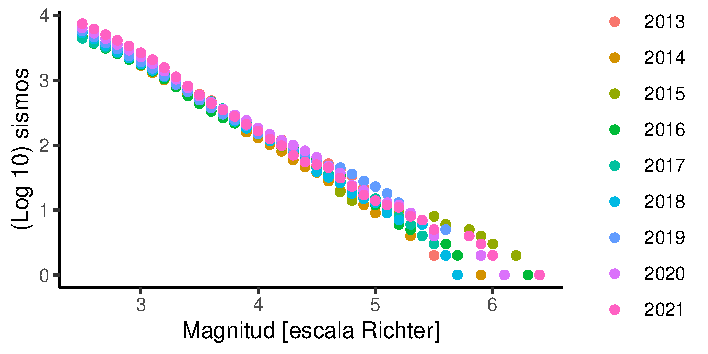
\includegraphics[width=0.5\textwidth]{acumulado_anual_magnitud.pdf}
\vspace{-0.8cm}
\caption{El apartamiento de la tendencia de la ley de Gutenberg-Richter en los sismos percibidos por la población muestra que la dificultad para que esto se produzca se incrementa con la baja de la magnitud.}
\label{fig:acumulado_anual_magnitud_percibidos}
%% \end{wrapfigure}
\end{figure}



\paragraph{Temporalidad de los percibidos}\label{sec:temporal}
Se puede hipotetizar que en los horarios de sueño nocturno sea menor la proporción de sismos percibidos.
Segmentando los registros con la variable Segundos del día (ver sección \ref{sec:formateo}) en intervalos de una hora se calculó la proporción entre casos percibidos o no.
Contrariando la hipótesis, en la figura \ref{fig:histograma_percibidos_por_hora} no parece posible identificar una banda horaria, e.g. noche, en la que la proporción sea menor.

\begin{figure}[!ht]
\centering
% Created by tikzDevice version 0.12.6 on 2024-06-18 13:23:29
% !TEX encoding = UTF-8 Unicode
\begin{tikzpicture}[x=1pt,y=1pt]
\definecolor{fillColor}{RGB}{255,255,255}
\path[use as bounding box,fill=fillColor,fill opacity=0.00] (0,0) rectangle (346.90,144.54);
\begin{scope}
\path[clip] (  0.00,  0.00) rectangle (346.90,144.54);
\definecolor{drawColor}{RGB}{255,255,255}
\definecolor{fillColor}{RGB}{255,255,255}

\path[draw=drawColor,line width= 0.6pt,line join=round,line cap=round,fill=fillColor] (  0.00,  0.00) rectangle (346.90,144.54);
\end{scope}
\begin{scope}
\path[clip] ( 27.31, 30.69) rectangle (341.40,139.04);
\definecolor{fillColor}{gray}{0.92}

\path[fill=fillColor] ( 27.31, 30.69) rectangle (341.40,139.04);
\definecolor{drawColor}{RGB}{255,255,255}

\path[draw=drawColor,line width= 0.3pt,line join=round] ( 27.31, 45.21) --
	(341.40, 45.21);

\path[draw=drawColor,line width= 0.3pt,line join=round] ( 27.31, 64.41) --
	(341.40, 64.41);

\path[draw=drawColor,line width= 0.3pt,line join=round] ( 27.31, 83.61) --
	(341.40, 83.61);

\path[draw=drawColor,line width= 0.3pt,line join=round] ( 27.31,102.81) --
	(341.40,102.81);

\path[draw=drawColor,line width= 0.3pt,line join=round] ( 27.31,122.01) --
	(341.40,122.01);

\path[draw=drawColor,line width= 0.3pt,line join=round] ( 76.83, 30.69) --
	( 76.83,139.04);

\path[draw=drawColor,line width= 0.3pt,line join=round] (136.57, 30.69) --
	(136.57,139.04);

\path[draw=drawColor,line width= 0.3pt,line join=round] (196.30, 30.69) --
	(196.30,139.04);

\path[draw=drawColor,line width= 0.3pt,line join=round] (256.04, 30.69) --
	(256.04,139.04);

\path[draw=drawColor,line width= 0.3pt,line join=round] (315.77, 30.69) --
	(315.77,139.04);

\path[draw=drawColor,line width= 0.6pt,line join=round] ( 27.31, 35.61) --
	(341.40, 35.61);

\path[draw=drawColor,line width= 0.6pt,line join=round] ( 27.31, 54.81) --
	(341.40, 54.81);

\path[draw=drawColor,line width= 0.6pt,line join=round] ( 27.31, 74.01) --
	(341.40, 74.01);

\path[draw=drawColor,line width= 0.6pt,line join=round] ( 27.31, 93.21) --
	(341.40, 93.21);

\path[draw=drawColor,line width= 0.6pt,line join=round] ( 27.31,112.41) --
	(341.40,112.41);

\path[draw=drawColor,line width= 0.6pt,line join=round] ( 27.31,131.61) --
	(341.40,131.61);

\path[draw=drawColor,line width= 0.6pt,line join=round] ( 46.97, 30.69) --
	( 46.97,139.04);

\path[draw=drawColor,line width= 0.6pt,line join=round] (106.70, 30.69) --
	(106.70,139.04);

\path[draw=drawColor,line width= 0.6pt,line join=round] (166.43, 30.69) --
	(166.43,139.04);

\path[draw=drawColor,line width= 0.6pt,line join=round] (226.17, 30.69) --
	(226.17,139.04);

\path[draw=drawColor,line width= 0.6pt,line join=round] (285.90, 30.69) --
	(285.90,139.04);
\definecolor{fillColor}{gray}{0.35}

\path[fill=fillColor] ( 41.59, 35.61) rectangle ( 52.34,129.73);

\path[fill=fillColor] ( 53.54, 35.61) rectangle ( 64.29,118.97);

\path[fill=fillColor] ( 65.48, 35.61) rectangle ( 76.24, 95.63);

\path[fill=fillColor] ( 77.43, 35.61) rectangle ( 88.18,100.38);

\path[fill=fillColor] ( 89.38, 35.61) rectangle (100.13,100.69);

\path[fill=fillColor] (101.32, 35.61) rectangle (112.08,104.15);

\path[fill=fillColor] (113.27, 35.61) rectangle (124.02,107.01);

\path[fill=fillColor] (125.22, 35.61) rectangle (135.97,101.17);

\path[fill=fillColor] (137.16, 35.61) rectangle (147.92,104.99);

\path[fill=fillColor] (149.11, 35.61) rectangle (159.86,107.58);

\path[fill=fillColor] (161.06, 35.61) rectangle (171.81,107.88);

\path[fill=fillColor] (173.01, 35.61) rectangle (183.76, 94.93);

\path[fill=fillColor] (184.95, 35.61) rectangle (195.70, 92.00);

\path[fill=fillColor] (196.90, 35.61) rectangle (207.65,110.31);

\path[fill=fillColor] (208.85, 35.61) rectangle (219.60, 99.88);

\path[fill=fillColor] (220.79, 35.61) rectangle (231.54, 94.61);

\path[fill=fillColor] (232.74, 35.61) rectangle (243.49, 90.40);

\path[fill=fillColor] (244.69, 35.61) rectangle (255.44,100.49);

\path[fill=fillColor] (256.63, 35.61) rectangle (267.39, 82.55);

\path[fill=fillColor] (268.58, 35.61) rectangle (279.33, 92.92);

\path[fill=fillColor] (280.53, 35.61) rectangle (291.28,107.55);

\path[fill=fillColor] (292.47, 35.61) rectangle (303.23,107.14);

\path[fill=fillColor] (304.42, 35.61) rectangle (315.17,104.05);

\path[fill=fillColor] (316.37, 35.61) rectangle (327.12,134.11);
\end{scope}
\begin{scope}
\path[clip] (  0.00,  0.00) rectangle (346.90,144.54);
\definecolor{drawColor}{gray}{0.30}

\node[text=drawColor,anchor=base east,inner sep=0pt, outer sep=0pt, scale=  0.88] at ( 22.36, 32.58) {0};

\node[text=drawColor,anchor=base east,inner sep=0pt, outer sep=0pt, scale=  0.88] at ( 22.36, 51.78) {1};

\node[text=drawColor,anchor=base east,inner sep=0pt, outer sep=0pt, scale=  0.88] at ( 22.36, 70.98) {2};

\node[text=drawColor,anchor=base east,inner sep=0pt, outer sep=0pt, scale=  0.88] at ( 22.36, 90.18) {3};

\node[text=drawColor,anchor=base east,inner sep=0pt, outer sep=0pt, scale=  0.88] at ( 22.36,109.38) {4};

\node[text=drawColor,anchor=base east,inner sep=0pt, outer sep=0pt, scale=  0.88] at ( 22.36,128.58) {5};
\end{scope}
\begin{scope}
\path[clip] (  0.00,  0.00) rectangle (346.90,144.54);
\definecolor{drawColor}{gray}{0.20}

\path[draw=drawColor,line width= 0.6pt,line join=round] ( 24.56, 35.61) --
	( 27.31, 35.61);

\path[draw=drawColor,line width= 0.6pt,line join=round] ( 24.56, 54.81) --
	( 27.31, 54.81);

\path[draw=drawColor,line width= 0.6pt,line join=round] ( 24.56, 74.01) --
	( 27.31, 74.01);

\path[draw=drawColor,line width= 0.6pt,line join=round] ( 24.56, 93.21) --
	( 27.31, 93.21);

\path[draw=drawColor,line width= 0.6pt,line join=round] ( 24.56,112.41) --
	( 27.31,112.41);

\path[draw=drawColor,line width= 0.6pt,line join=round] ( 24.56,131.61) --
	( 27.31,131.61);
\end{scope}
\begin{scope}
\path[clip] (  0.00,  0.00) rectangle (346.90,144.54);
\definecolor{drawColor}{gray}{0.20}

\path[draw=drawColor,line width= 0.6pt,line join=round] ( 46.97, 27.94) --
	( 46.97, 30.69);

\path[draw=drawColor,line width= 0.6pt,line join=round] (106.70, 27.94) --
	(106.70, 30.69);

\path[draw=drawColor,line width= 0.6pt,line join=round] (166.43, 27.94) --
	(166.43, 30.69);

\path[draw=drawColor,line width= 0.6pt,line join=round] (226.17, 27.94) --
	(226.17, 30.69);

\path[draw=drawColor,line width= 0.6pt,line join=round] (285.90, 27.94) --
	(285.90, 30.69);
\end{scope}
\begin{scope}
\path[clip] (  0.00,  0.00) rectangle (346.90,144.54);
\definecolor{drawColor}{gray}{0.30}

\node[text=drawColor,anchor=base,inner sep=0pt, outer sep=0pt, scale=  0.88] at ( 46.97, 19.68) {0};

\node[text=drawColor,anchor=base,inner sep=0pt, outer sep=0pt, scale=  0.88] at (106.70, 19.68) {5};

\node[text=drawColor,anchor=base,inner sep=0pt, outer sep=0pt, scale=  0.88] at (166.43, 19.68) {10};

\node[text=drawColor,anchor=base,inner sep=0pt, outer sep=0pt, scale=  0.88] at (226.17, 19.68) {15};

\node[text=drawColor,anchor=base,inner sep=0pt, outer sep=0pt, scale=  0.88] at (285.90, 19.68) {20};
\end{scope}
\begin{scope}
\path[clip] (  0.00,  0.00) rectangle (346.90,144.54);
\definecolor{drawColor}{RGB}{0,0,0}

\node[text=drawColor,anchor=base,inner sep=0pt, outer sep=0pt, scale=  1.10] at (184.35,  7.64) {Hora};
\end{scope}
\begin{scope}
\path[clip] (  0.00,  0.00) rectangle (346.90,144.54);
\definecolor{drawColor}{RGB}{0,0,0}

\node[text=drawColor,rotate= 90.00,anchor=base,inner sep=0pt, outer sep=0pt, scale=  1.10] at ( 13.08, 84.86) {Percibidos [\%]};
\end{scope}
\end{tikzpicture}

\vspace{-0.8cm}
\caption{Proporción de sismos percibidos por la población en función de la hora del día.}
\label{fig:histograma_percibidos_por_hora}
\end{figure}

Otra hipótesis que puede formularse es que en los meses de verano, enero y febrero, sea menor la proporción de sismos percibidos asumiendo que la población tiene más horas de actividades al aire libre, y es en interiores de construcciones altas donde más fácilmente se perciben los sismos \cite{noauthor_intensidad_2022}.
Sin embargo la figura \ref{fig:percibidos_trimestre_histrograma} muestra que en el primer trimestre se halla la mayor proporción de sismos percibidos.

\begin{figure}[!ht]
	\centering
	% Created by tikzDevice version 0.12.6 on 2024-07-06 15:55:57
% !TEX encoding = UTF-8 Unicode
\begin{tikzpicture}[x=1pt,y=1pt]
\definecolor{fillColor}{RGB}{255,255,255}
\path[use as bounding box,fill=fillColor,fill opacity=0.00] (0,0) rectangle (346.90,144.54);
\begin{scope}
\path[clip] (  0.00,  0.00) rectangle (346.90,144.54);
\definecolor{drawColor}{RGB}{255,255,255}
\definecolor{fillColor}{RGB}{255,255,255}

\path[draw=drawColor,line width= 0.6pt,line join=round,line cap=round,fill=fillColor] (  0.00,  0.00) rectangle (346.90,144.54);
\end{scope}
\begin{scope}
\path[clip] ( 27.31, 30.69) rectangle (341.40,139.04);
\definecolor{fillColor}{gray}{0.92}

\path[fill=fillColor] ( 27.31, 30.69) rectangle (341.40,139.04);
\definecolor{drawColor}{RGB}{255,255,255}

\path[draw=drawColor,line width= 0.3pt,line join=round] ( 27.31, 54.04) --
	(341.40, 54.04);

\path[draw=drawColor,line width= 0.3pt,line join=round] ( 27.31, 90.91) --
	(341.40, 90.91);

\path[draw=drawColor,line width= 0.3pt,line join=round] ( 27.31,127.77) --
	(341.40,127.77);

\path[draw=drawColor,line width= 0.3pt,line join=round] ( 37.93, 30.69) --
	( 37.93,139.04);

\path[draw=drawColor,line width= 0.3pt,line join=round] (111.14, 30.69) --
	(111.14,139.04);

\path[draw=drawColor,line width= 0.3pt,line join=round] (184.35, 30.69) --
	(184.35,139.04);

\path[draw=drawColor,line width= 0.3pt,line join=round] (257.57, 30.69) --
	(257.57,139.04);

\path[draw=drawColor,line width= 0.3pt,line join=round] (330.78, 30.69) --
	(330.78,139.04);

\path[draw=drawColor,line width= 0.6pt,line join=round] ( 27.31, 35.61) --
	(341.40, 35.61);

\path[draw=drawColor,line width= 0.6pt,line join=round] ( 27.31, 72.47) --
	(341.40, 72.47);

\path[draw=drawColor,line width= 0.6pt,line join=round] ( 27.31,109.34) --
	(341.40,109.34);

\path[draw=drawColor,line width= 0.6pt,line join=round] ( 74.54, 30.69) --
	( 74.54,139.04);

\path[draw=drawColor,line width= 0.6pt,line join=round] (147.75, 30.69) --
	(147.75,139.04);

\path[draw=drawColor,line width= 0.6pt,line join=round] (220.96, 30.69) --
	(220.96,139.04);

\path[draw=drawColor,line width= 0.6pt,line join=round] (294.17, 30.69) --
	(294.17,139.04);
\definecolor{fillColor}{gray}{0.35}

\path[fill=fillColor] ( 41.59, 35.61) rectangle (107.48,134.11);

\path[fill=fillColor] (114.80, 35.61) rectangle (180.69,112.34);

\path[fill=fillColor] (188.02, 35.61) rectangle (253.91, 96.82);

\path[fill=fillColor] (261.23, 35.61) rectangle (327.12,107.18);
\end{scope}
\begin{scope}
\path[clip] (  0.00,  0.00) rectangle (346.90,144.54);
\definecolor{drawColor}{gray}{0.30}

\node[text=drawColor,anchor=base east,inner sep=0pt, outer sep=0pt, scale=  0.88] at ( 22.36, 32.58) {0};

\node[text=drawColor,anchor=base east,inner sep=0pt, outer sep=0pt, scale=  0.88] at ( 22.36, 69.44) {1};

\node[text=drawColor,anchor=base east,inner sep=0pt, outer sep=0pt, scale=  0.88] at ( 22.36,106.31) {2};
\end{scope}
\begin{scope}
\path[clip] (  0.00,  0.00) rectangle (346.90,144.54);
\definecolor{drawColor}{gray}{0.20}

\path[draw=drawColor,line width= 0.6pt,line join=round] ( 24.56, 35.61) --
	( 27.31, 35.61);

\path[draw=drawColor,line width= 0.6pt,line join=round] ( 24.56, 72.47) --
	( 27.31, 72.47);

\path[draw=drawColor,line width= 0.6pt,line join=round] ( 24.56,109.34) --
	( 27.31,109.34);
\end{scope}
\begin{scope}
\path[clip] (  0.00,  0.00) rectangle (346.90,144.54);
\definecolor{drawColor}{gray}{0.20}

\path[draw=drawColor,line width= 0.6pt,line join=round] ( 74.54, 27.94) --
	( 74.54, 30.69);

\path[draw=drawColor,line width= 0.6pt,line join=round] (147.75, 27.94) --
	(147.75, 30.69);

\path[draw=drawColor,line width= 0.6pt,line join=round] (220.96, 27.94) --
	(220.96, 30.69);

\path[draw=drawColor,line width= 0.6pt,line join=round] (294.17, 27.94) --
	(294.17, 30.69);
\end{scope}
\begin{scope}
\path[clip] (  0.00,  0.00) rectangle (346.90,144.54);
\definecolor{drawColor}{gray}{0.30}

\node[text=drawColor,anchor=base,inner sep=0pt, outer sep=0pt, scale=  0.88] at ( 74.54, 19.68) {1};

\node[text=drawColor,anchor=base,inner sep=0pt, outer sep=0pt, scale=  0.88] at (147.75, 19.68) {2};

\node[text=drawColor,anchor=base,inner sep=0pt, outer sep=0pt, scale=  0.88] at (220.96, 19.68) {3};

\node[text=drawColor,anchor=base,inner sep=0pt, outer sep=0pt, scale=  0.88] at (294.17, 19.68) {4};
\end{scope}
\begin{scope}
\path[clip] (  0.00,  0.00) rectangle (346.90,144.54);
\definecolor{drawColor}{RGB}{0,0,0}

\node[text=drawColor,rotate= 90.00,anchor=base,inner sep=0pt, outer sep=0pt, scale=  1.10] at ( 13.08, 84.86) {Percibidos [\%]};
\end{scope}
\end{tikzpicture}

	\vspace{-0.8cm}
	\caption{Proporción de sismos percibidos por trimestre.}
	\label{fig:percibidos_trimestre_histrograma}
\end{figure}

Con el fin de explorar si los apartamientos trimestrales en las proporciones son significativos se realizar un \emph{ensayo binomial} de cada proporción trimestral contra la media.
Este se alimenta con la tabla de contingencia de la figura \ref{fig:tabla_contingencia_trimestre} que muestra una cantidad de muestras que se consideran suficientes para proceder con el ensayo.

\begin{table}[!ht]
	\centering
	\begin{tabular}{lcccc}
		\toprule
		Trimestre & 1.ero & 2.do & 3.ero & 4.to \\
		\midrule
		Percibido & 215 & 154 & 112 & 138 \\
		No percibido & 8046 & 7399 & 6745 & 7108 \\
		\bottomrule
	\end{tabular}
	\caption{Tabla de contingencia de sismos percibidos por trimestre.}
	\label{fig:tabla_contingencia_trimestre}
\end{table}

Para el primer y tercer cuatrimestre se obtuvieron valores p de \(0.000452\) y \(0.016623\) respectivamente, lo que indica que las proporciones de sismos percibidos en estos trimestres son significativamente distintas de la media.
No se tiene una explicación para esta observación, que debe aclararse, debe tomarse con precaución pues se realiza sobre un número muy limitado de proporciones.

Dado que se son apreciables variaciones interanuales en el número total de terremotos, como lo evidencia la figura \ref{fig:acumulado_anual_magnitud}, tal vez debieran tomarse los trimestres de cada año en forma independientes años y analizar su medía y dispersión.
Pero es posible que el número de muestras en cada trimestre sea insuficiente para obtener resultados representativos. 



\section{Ingeniería de características}\label{sec:ingeniería}
% \section{Descripción de las técnicas de análisis y, si corresponde, de modelado}


%\section{Ingeniería de características}\label{sec:ingeniería}

%Por otra parte el preprocesamiento comprende la generación de nuevas variables a partir de las existentes que se consideren relevantes para el análisis, lo que recibe el nombre de ingeniería de características (feature engineering).

%Esto comprende tareas de distinta naturaleza.
%Por un lado las que se realizan para adecuar el formato de datos para las herramientas a utilizar como el que se describe en el próximo párrafo.
%Otras de estas es una modificación basada en un conocimiento del sistema que genera los datos.
% En estos casos se hace uso de un criterio que parte de condicionamientos sobre el sistema físico o se implementa un modelo en base a la física del sistema.
% Dos de las variables de este conjunto de datos son afectadas por este tipo de modificación, que se describe posteriormente en una subsección.

% Se generaron dos nuevas columnas a partir de las existentes en el conjunto de datos original, una en función al formato de los datos en la columna \lstinline[language = R]'Hora' y otra en función de la escala física utilizada en la columna \lstinline[language = R]'Magnitud'.


\subsection{Descarte de terremotos de poca profundidad}
% \paragraph{Recorte de poca profundidad}

Hay sismos cuyo origen no son terremotos sino desplazamientos superficiales de tierra, explosiones para la minera o el fracturado hidráulico para la extracción de hidrocarburos.
Se busca omitir tales orígenes en los datos informados.

Siendo que la variable se informa como enteros de kilómetros, estos representarían los hipocentros hasta una profundidad de \SI{500}{\metre}, compatibles con estas actividades artificiales.
La omisión de estas fuentes a baja profundidad es una práctica usual en el análisis de datos orientados a sismos originados en terremotos \cite{hu_applying_2024}.
El pequeño número que estos representan  en el conjunto de datos se aprecia en el histograma de profundidad que reproduce la figura \ref{fig:histograma_profundidad50km}.
Son filtrados con la instrucción \lstinline[language = R]'sismos_SJ <- sismos_SJ[Profundidad > 0]'.
\begin{figure}[!ht]
% \begin{wrapfigure}[22]{r}[10pt]{0.48\textwidth}
	\centering
  \vspace{-1.5cm} % Adjust the value as needed
	% Created by tikzDevice version 0.12.6 on 2024-07-05 15:51:11
% !TEX encoding = UTF-8 Unicode
\begin{tikzpicture}[x=1pt,y=1pt]
\definecolor{fillColor}{RGB}{255,255,255}
\path[use as bounding box,fill=fillColor,fill opacity=0.00] (0,0) rectangle (361.35,289.08);
\begin{scope}
\path[clip] (  0.00,  0.00) rectangle (361.35,289.08);
\definecolor{drawColor}{RGB}{0,0,0}

\node[text=drawColor,anchor=base,inner sep=0pt, outer sep=0pt, scale=  1.20] at (192.68, 15.60) {Profundidad [km]};

\node[text=drawColor,rotate= 90.00,anchor=base,inner sep=0pt, outer sep=0pt, scale=  1.20] at ( 10.80,150.54) {Frecuencia};
\end{scope}
\begin{scope}
\path[clip] (  0.00,  0.00) rectangle (361.35,289.08);
\definecolor{drawColor}{RGB}{0,0,0}

\path[draw=drawColor,line width= 0.4pt,line join=round,line cap=round] ( 59.83, 61.20) -- (290.87, 61.20);

\path[draw=drawColor,line width= 0.4pt,line join=round,line cap=round] ( 59.83, 61.20) -- ( 59.83, 55.20);

\path[draw=drawColor,line width= 0.4pt,line join=round,line cap=round] (117.59, 61.20) -- (117.59, 55.20);

\path[draw=drawColor,line width= 0.4pt,line join=round,line cap=round] (175.35, 61.20) -- (175.35, 55.20);

\path[draw=drawColor,line width= 0.4pt,line join=round,line cap=round] (233.11, 61.20) -- (233.11, 55.20);

\path[draw=drawColor,line width= 0.4pt,line join=round,line cap=round] (290.87, 61.20) -- (290.87, 55.20);

\node[text=drawColor,anchor=base,inner sep=0pt, outer sep=0pt, scale=  1.20] at ( 59.83, 39.60) {0};

\node[text=drawColor,anchor=base,inner sep=0pt, outer sep=0pt, scale=  1.20] at (117.59, 39.60) {10};

\node[text=drawColor,anchor=base,inner sep=0pt, outer sep=0pt, scale=  1.20] at (175.35, 39.60) {20};

\node[text=drawColor,anchor=base,inner sep=0pt, outer sep=0pt, scale=  1.20] at (233.11, 39.60) {30};

\node[text=drawColor,anchor=base,inner sep=0pt, outer sep=0pt, scale=  1.20] at (290.87, 39.60) {40};

\path[draw=drawColor,line width= 0.4pt,line join=round,line cap=round] ( 49.20, 67.82) -- ( 49.20,235.14);

\path[draw=drawColor,line width= 0.4pt,line join=round,line cap=round] ( 49.20, 67.82) -- ( 43.20, 67.82);

\path[draw=drawColor,line width= 0.4pt,line join=round,line cap=round] ( 49.20,109.65) -- ( 43.20,109.65);

\path[draw=drawColor,line width= 0.4pt,line join=round,line cap=round] ( 49.20,151.48) -- ( 43.20,151.48);

\path[draw=drawColor,line width= 0.4pt,line join=round,line cap=round] ( 49.20,193.31) -- ( 43.20,193.31);

\path[draw=drawColor,line width= 0.4pt,line join=round,line cap=round] ( 49.20,235.14) -- ( 43.20,235.14);

\node[text=drawColor,rotate= 90.00,anchor=base,inner sep=0pt, outer sep=0pt, scale=  1.20] at ( 34.80, 67.82) {0};

\node[text=drawColor,rotate= 90.00,anchor=base,inner sep=0pt, outer sep=0pt, scale=  1.20] at ( 34.80,109.65) {200};

\node[text=drawColor,rotate= 90.00,anchor=base,inner sep=0pt, outer sep=0pt, scale=  1.20] at ( 34.80,151.48) {400};

\node[text=drawColor,rotate= 90.00,anchor=base,inner sep=0pt, outer sep=0pt, scale=  1.20] at ( 34.80,193.31) {600};

\node[text=drawColor,rotate= 90.00,anchor=base,inner sep=0pt, outer sep=0pt, scale=  1.20] at ( 34.80,235.14) {800};
\end{scope}
\begin{scope}
\path[clip] ( 49.20, 61.20) rectangle (336.15,239.88);
\definecolor{drawColor}{RGB}{0,0,0}
\definecolor{fillColor}{RGB}{211,211,211}

\path[draw=drawColor,line width= 0.4pt,line join=round,line cap=round,fill=fillColor] ( 59.83, 67.82) rectangle ( 65.60, 68.03);

\path[draw=drawColor,line width= 0.4pt,line join=round,line cap=round,fill=fillColor] ( 65.60, 67.82) rectangle ( 71.38, 69.07);

\path[draw=drawColor,line width= 0.4pt,line join=round,line cap=round,fill=fillColor] ( 71.38, 67.82) rectangle ( 77.16, 70.96);

\path[draw=drawColor,line width= 0.4pt,line join=round,line cap=round,fill=fillColor] ( 77.16, 67.82) rectangle ( 82.93, 72.84);

\path[draw=drawColor,line width= 0.4pt,line join=round,line cap=round,fill=fillColor] ( 82.93, 67.82) rectangle ( 88.71, 80.16);

\path[draw=drawColor,line width= 0.4pt,line join=round,line cap=round,fill=fillColor] ( 88.71, 67.82) rectangle ( 94.48, 93.96);

\path[draw=drawColor,line width= 0.4pt,line join=round,line cap=round,fill=fillColor] ( 94.48, 67.82) rectangle (100.26,106.30);

\path[draw=drawColor,line width= 0.4pt,line join=round,line cap=round,fill=fillColor] (100.26, 67.82) rectangle (106.04,108.39);

\path[draw=drawColor,line width= 0.4pt,line join=round,line cap=round,fill=fillColor] (106.04, 67.82) rectangle (111.81,106.93);

\path[draw=drawColor,line width= 0.4pt,line join=round,line cap=round,fill=fillColor] (111.81, 67.82) rectangle (117.59,233.26);

\path[draw=drawColor,line width= 0.4pt,line join=round,line cap=round,fill=fillColor] (117.59, 67.82) rectangle (123.36,111.32);

\path[draw=drawColor,line width= 0.4pt,line join=round,line cap=round,fill=fillColor] (123.36, 67.82) rectangle (129.14,108.39);

\path[draw=drawColor,line width= 0.4pt,line join=round,line cap=round,fill=fillColor] (129.14, 67.82) rectangle (134.92,102.54);

\path[draw=drawColor,line width= 0.4pt,line join=round,line cap=round,fill=fillColor] (134.92, 67.82) rectangle (140.69,105.47);

\path[draw=drawColor,line width= 0.4pt,line join=round,line cap=round,fill=fillColor] (140.69, 67.82) rectangle (146.47,100.03);

\path[draw=drawColor,line width= 0.4pt,line join=round,line cap=round,fill=fillColor] (146.47, 67.82) rectangle (152.24, 92.29);

\path[draw=drawColor,line width= 0.4pt,line join=round,line cap=round,fill=fillColor] (152.24, 67.82) rectangle (158.02, 89.36);

\path[draw=drawColor,line width= 0.4pt,line join=round,line cap=round,fill=fillColor] (158.02, 67.82) rectangle (163.80, 87.48);

\path[draw=drawColor,line width= 0.4pt,line join=round,line cap=round,fill=fillColor] (163.80, 67.82) rectangle (169.57, 86.43);

\path[draw=drawColor,line width= 0.4pt,line join=round,line cap=round,fill=fillColor] (169.57, 67.82) rectangle (175.35, 92.29);

\path[draw=drawColor,line width= 0.4pt,line join=round,line cap=round,fill=fillColor] (175.35, 67.82) rectangle (181.12, 86.43);

\path[draw=drawColor,line width= 0.4pt,line join=round,line cap=round,fill=fillColor] (181.12, 67.82) rectangle (186.90, 86.64);

\path[draw=drawColor,line width= 0.4pt,line join=round,line cap=round,fill=fillColor] (186.90, 67.82) rectangle (192.68, 86.22);

\path[draw=drawColor,line width= 0.4pt,line join=round,line cap=round,fill=fillColor] (192.68, 67.82) rectangle (198.45, 83.09);

\path[draw=drawColor,line width= 0.4pt,line join=round,line cap=round,fill=fillColor] (198.45, 67.82) rectangle (204.23, 86.64);

\path[draw=drawColor,line width= 0.4pt,line join=round,line cap=round,fill=fillColor] (204.23, 67.82) rectangle (210.00, 80.37);

\path[draw=drawColor,line width= 0.4pt,line join=round,line cap=round,fill=fillColor] (210.00, 67.82) rectangle (215.78, 79.95);

\path[draw=drawColor,line width= 0.4pt,line join=round,line cap=round,fill=fillColor] (215.78, 67.82) rectangle (221.55, 78.28);

\path[draw=drawColor,line width= 0.4pt,line join=round,line cap=round,fill=fillColor] (221.55, 67.82) rectangle (227.33, 78.07);

\path[draw=drawColor,line width= 0.4pt,line join=round,line cap=round,fill=fillColor] (227.33, 67.82) rectangle (233.11, 82.25);

\path[draw=drawColor,line width= 0.4pt,line join=round,line cap=round,fill=fillColor] (233.11, 67.82) rectangle (238.88, 73.88);

\path[draw=drawColor,line width= 0.4pt,line join=round,line cap=round,fill=fillColor] (238.88, 67.82) rectangle (244.66, 75.14);

\path[draw=drawColor,line width= 0.4pt,line join=round,line cap=round,fill=fillColor] (244.66, 67.82) rectangle (250.43, 74.51);

\path[draw=drawColor,line width= 0.4pt,line join=round,line cap=round,fill=fillColor] (250.43, 67.82) rectangle (256.21, 74.30);

\path[draw=drawColor,line width= 0.4pt,line join=round,line cap=round,fill=fillColor] (256.21, 67.82) rectangle (261.99, 72.84);

\path[draw=drawColor,line width= 0.4pt,line join=round,line cap=round,fill=fillColor] (261.99, 67.82) rectangle (267.76, 70.12);

\path[draw=drawColor,line width= 0.4pt,line join=round,line cap=round,fill=fillColor] (267.76, 67.82) rectangle (273.54, 71.58);

\path[draw=drawColor,line width= 0.4pt,line join=round,line cap=round,fill=fillColor] (273.54, 67.82) rectangle (279.31, 70.54);

\path[draw=drawColor,line width= 0.4pt,line join=round,line cap=round,fill=fillColor] (279.31, 67.82) rectangle (285.09, 69.49);

\path[draw=drawColor,line width= 0.4pt,line join=round,line cap=round,fill=fillColor] (285.09, 67.82) rectangle (290.87, 75.35);

\path[draw=drawColor,line width= 0.4pt,line join=round,line cap=round,fill=fillColor] (290.87, 67.82) rectangle (296.64, 68.86);

\path[draw=drawColor,line width= 0.4pt,line join=round,line cap=round,fill=fillColor] (296.64, 67.82) rectangle (302.42, 68.24);

\path[draw=drawColor,line width= 0.4pt,line join=round,line cap=round,fill=fillColor] (302.42, 67.82) rectangle (308.19, 68.24);

\path[draw=drawColor,line width= 0.4pt,line join=round,line cap=round,fill=fillColor] (308.19, 67.82) rectangle (313.97, 68.65);

\path[draw=drawColor,line width= 0.4pt,line join=round,line cap=round,fill=fillColor] (313.97, 67.82) rectangle (319.75, 68.03);

\path[draw=drawColor,line width= 0.4pt,line join=round,line cap=round,fill=fillColor] (319.75, 67.82) rectangle (325.52, 68.24);
\end{scope}
\end{tikzpicture}

	% 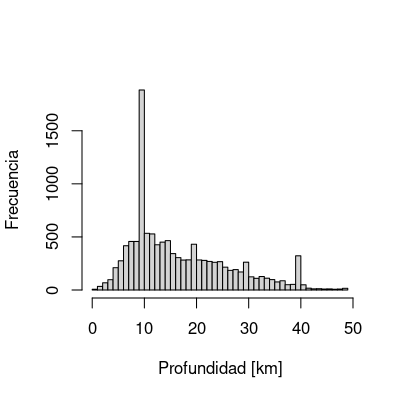
\includegraphics[width=0.4\textwidth]{histograma_profundidad_menos50.png}
  \vspace{-1cm} % Adjust the value as needed
	\caption{Los sismos con origen a profundidad de \SI{0}{\kilo\metre} son pocos en el conjunto de datos de terremotos con hipocentros poco profundos, < \SI{50}{\kilo\metre}.}
	\label{fig:histograma_profundidad50km}
% \end{wrapfigure}
\end{figure}

Este recorte tiene un efecto cuasi-irrelevante en la distribución de la profundidad de los terremotos en el conjunto de datos para San Juan. 
La figura \ref{fig:histograma_profundidad50km} mostró que los hay con \(h < \SI{50}{\kilo\metre}\), pero los hay hasta con \(h= \SI{750}{\kilo\metre}\) siendo los de \(h > \SI{50}{\kilo\metre}\) \(\approx 79\%\) del total como evidencia el histograma que reproduce la figura \ref{fig:histograma_profundidad750km}.

\begin{figure}[!ht]
% \begin{wrapfigure}[22]{r}[10pt]{0.48\textwidth}
	\centering
  \vspace{-1.5cm} % Adjust the value as needed
	% Created by tikzDevice version 0.12.6 on 2024-07-05 15:51:28
% !TEX encoding = UTF-8 Unicode
\begin{tikzpicture}[x=1pt,y=1pt]
\definecolor{fillColor}{RGB}{255,255,255}
\path[use as bounding box,fill=fillColor,fill opacity=0.00] (0,0) rectangle (361.35,289.08);
\begin{scope}
\path[clip] (  0.00,  0.00) rectangle (361.35,289.08);
\definecolor{drawColor}{RGB}{0,0,0}

\node[text=drawColor,anchor=base,inner sep=0pt, outer sep=0pt, scale=  1.20] at (192.68, 15.60) {Profundidad [km]};

\node[text=drawColor,rotate= 90.00,anchor=base,inner sep=0pt, outer sep=0pt, scale=  1.20] at ( 10.80,150.54) {Frecuencia};
\end{scope}
\begin{scope}
\path[clip] (  0.00,  0.00) rectangle (361.35,289.08);
\definecolor{drawColor}{RGB}{0,0,0}

\path[draw=drawColor,line width= 0.4pt,line join=round,line cap=round] ( 59.83, 61.20) -- (296.00, 61.20);

\path[draw=drawColor,line width= 0.4pt,line join=round,line cap=round] ( 59.83, 61.20) -- ( 59.83, 55.20);

\path[draw=drawColor,line width= 0.4pt,line join=round,line cap=round] (118.87, 61.20) -- (118.87, 55.20);

\path[draw=drawColor,line width= 0.4pt,line join=round,line cap=round] (177.91, 61.20) -- (177.91, 55.20);

\path[draw=drawColor,line width= 0.4pt,line join=round,line cap=round] (236.96, 61.20) -- (236.96, 55.20);

\path[draw=drawColor,line width= 0.4pt,line join=round,line cap=round] (296.00, 61.20) -- (296.00, 55.20);

\node[text=drawColor,anchor=base,inner sep=0pt, outer sep=0pt, scale=  1.20] at ( 59.83, 39.60) {0};

\node[text=drawColor,anchor=base,inner sep=0pt, outer sep=0pt, scale=  1.20] at (118.87, 39.60) {100};

\node[text=drawColor,anchor=base,inner sep=0pt, outer sep=0pt, scale=  1.20] at (177.91, 39.60) {200};

\node[text=drawColor,anchor=base,inner sep=0pt, outer sep=0pt, scale=  1.20] at (236.96, 39.60) {300};

\node[text=drawColor,anchor=base,inner sep=0pt, outer sep=0pt, scale=  1.20] at (296.00, 39.60) {400};

\path[draw=drawColor,line width= 0.4pt,line join=round,line cap=round] ( 49.20, 67.82) -- ( 49.20,222.89);

\path[draw=drawColor,line width= 0.4pt,line join=round,line cap=round] ( 49.20, 67.82) -- ( 43.20, 67.82);

\path[draw=drawColor,line width= 0.4pt,line join=round,line cap=round] ( 49.20, 93.66) -- ( 43.20, 93.66);

\path[draw=drawColor,line width= 0.4pt,line join=round,line cap=round] ( 49.20,119.51) -- ( 43.20,119.51);

\path[draw=drawColor,line width= 0.4pt,line join=round,line cap=round] ( 49.20,145.35) -- ( 43.20,145.35);

\path[draw=drawColor,line width= 0.4pt,line join=round,line cap=round] ( 49.20,171.20) -- ( 43.20,171.20);

\path[draw=drawColor,line width= 0.4pt,line join=round,line cap=round] ( 49.20,197.04) -- ( 43.20,197.04);

\path[draw=drawColor,line width= 0.4pt,line join=round,line cap=round] ( 49.20,222.89) -- ( 43.20,222.89);

\node[text=drawColor,rotate= 90.00,anchor=base,inner sep=0pt, outer sep=0pt, scale=  1.20] at ( 34.80, 67.82) {0};

\node[text=drawColor,rotate= 90.00,anchor=base,inner sep=0pt, outer sep=0pt, scale=  1.20] at ( 34.80, 93.66) {2000};

\node[text=drawColor,rotate= 90.00,anchor=base,inner sep=0pt, outer sep=0pt, scale=  1.20] at ( 34.80,145.35) {6000};

\node[text=drawColor,rotate= 90.00,anchor=base,inner sep=0pt, outer sep=0pt, scale=  1.20] at ( 34.80,197.04) {10000};
\end{scope}
\begin{scope}
\path[clip] ( 49.20, 61.20) rectangle (336.15,239.88);
\definecolor{drawColor}{RGB}{0,0,0}
\definecolor{fillColor}{RGB}{211,211,211}

\path[draw=drawColor,line width= 0.4pt,line join=round,line cap=round,fill=fillColor] ( 59.83, 67.82) rectangle ( 65.73, 88.31);

\path[draw=drawColor,line width= 0.4pt,line join=round,line cap=round,fill=fillColor] ( 65.73, 67.82) rectangle ( 71.64, 86.19);

\path[draw=drawColor,line width= 0.4pt,line join=round,line cap=round,fill=fillColor] ( 71.64, 67.82) rectangle ( 77.54, 77.07);

\path[draw=drawColor,line width= 0.4pt,line join=round,line cap=round,fill=fillColor] ( 77.54, 67.82) rectangle ( 83.45, 70.88);

\path[draw=drawColor,line width= 0.4pt,line join=round,line cap=round,fill=fillColor] ( 83.45, 67.82) rectangle ( 89.35, 68.06);

\path[draw=drawColor,line width= 0.4pt,line join=round,line cap=round,fill=fillColor] ( 89.35, 67.82) rectangle ( 95.25, 67.95);

\path[draw=drawColor,line width= 0.4pt,line join=round,line cap=round,fill=fillColor] ( 95.25, 67.82) rectangle (101.16, 68.01);

\path[draw=drawColor,line width= 0.4pt,line join=round,line cap=round,fill=fillColor] (101.16, 67.82) rectangle (107.06, 68.18);

\path[draw=drawColor,line width= 0.4pt,line join=round,line cap=round,fill=fillColor] (107.06, 67.82) rectangle (112.97, 69.61);

\path[draw=drawColor,line width= 0.4pt,line join=round,line cap=round,fill=fillColor] (112.97, 67.82) rectangle (118.87,111.60);

\path[draw=drawColor,line width= 0.4pt,line join=round,line cap=round,fill=fillColor] (118.87, 67.82) rectangle (124.78,233.26);

\path[draw=drawColor,line width= 0.4pt,line join=round,line cap=round,fill=fillColor] (124.78, 67.82) rectangle (130.68,155.69);

\path[draw=drawColor,line width= 0.4pt,line join=round,line cap=round,fill=fillColor] (130.68, 67.82) rectangle (136.58, 96.29);

\path[draw=drawColor,line width= 0.4pt,line join=round,line cap=round,fill=fillColor] (136.58, 67.82) rectangle (142.49, 73.00);

\path[draw=drawColor,line width= 0.4pt,line join=round,line cap=round,fill=fillColor] (142.49, 67.82) rectangle (148.39, 68.74);

\path[draw=drawColor,line width= 0.4pt,line join=round,line cap=round,fill=fillColor] (148.39, 67.82) rectangle (154.30, 68.18);

\path[draw=drawColor,line width= 0.4pt,line join=round,line cap=round,fill=fillColor] (154.30, 67.82) rectangle (160.20, 67.96);

\path[draw=drawColor,line width= 0.4pt,line join=round,line cap=round,fill=fillColor] (160.20, 67.82) rectangle (166.11, 67.86);

\path[draw=drawColor,line width= 0.4pt,line join=round,line cap=round,fill=fillColor] (166.11, 67.82) rectangle (172.01, 67.91);

\path[draw=drawColor,line width= 0.4pt,line join=round,line cap=round,fill=fillColor] (172.01, 67.82) rectangle (177.91, 67.87);

\path[draw=drawColor,line width= 0.4pt,line join=round,line cap=round,fill=fillColor] (177.91, 67.82) rectangle (183.82, 67.84);

\path[draw=drawColor,line width= 0.4pt,line join=round,line cap=round,fill=fillColor] (183.82, 67.82) rectangle (189.72, 67.86);

\path[draw=drawColor,line width= 0.4pt,line join=round,line cap=round,fill=fillColor] (189.72, 67.82) rectangle (195.63, 67.84);

\path[draw=drawColor,line width= 0.4pt,line join=round,line cap=round,fill=fillColor] (195.63, 67.82) rectangle (201.53, 67.87);

\path[draw=drawColor,line width= 0.4pt,line join=round,line cap=round,fill=fillColor] (201.53, 67.82) rectangle (207.44, 67.84);

\path[draw=drawColor,line width= 0.4pt,line join=round,line cap=round,fill=fillColor] (207.44, 67.82) rectangle (213.34, 67.84);

\path[draw=drawColor,line width= 0.4pt,line join=round,line cap=round,fill=fillColor] (213.34, 67.82) rectangle (219.24, 67.82);

\path[draw=drawColor,line width= 0.4pt,line join=round,line cap=round,fill=fillColor] (219.24, 67.82) rectangle (225.15, 67.84);

\path[draw=drawColor,line width= 0.4pt,line join=round,line cap=round,fill=fillColor] (225.15, 67.82) rectangle (231.05, 67.84);

\path[draw=drawColor,line width= 0.4pt,line join=round,line cap=round,fill=fillColor] (231.05, 67.82) rectangle (236.96, 67.82);

\path[draw=drawColor,line width= 0.4pt,line join=round,line cap=round,fill=fillColor] (236.96, 67.82) rectangle (242.86, 67.82);

\path[draw=drawColor,line width= 0.4pt,line join=round,line cap=round,fill=fillColor] (242.86, 67.82) rectangle (248.77, 67.83);

\path[draw=drawColor,line width= 0.4pt,line join=round,line cap=round,fill=fillColor] (248.77, 67.82) rectangle (254.67, 67.82);

\path[draw=drawColor,line width= 0.4pt,line join=round,line cap=round,fill=fillColor] (254.67, 67.82) rectangle (260.57, 67.82);

\path[draw=drawColor,line width= 0.4pt,line join=round,line cap=round,fill=fillColor] (260.57, 67.82) rectangle (266.48, 67.82);

\path[draw=drawColor,line width= 0.4pt,line join=round,line cap=round,fill=fillColor] (266.48, 67.82) rectangle (272.38, 67.82);

\path[draw=drawColor,line width= 0.4pt,line join=round,line cap=round,fill=fillColor] (272.38, 67.82) rectangle (278.29, 67.82);

\path[draw=drawColor,line width= 0.4pt,line join=round,line cap=round,fill=fillColor] (278.29, 67.82) rectangle (284.19, 67.82);

\path[draw=drawColor,line width= 0.4pt,line join=round,line cap=round,fill=fillColor] (284.19, 67.82) rectangle (290.10, 67.82);

\path[draw=drawColor,line width= 0.4pt,line join=round,line cap=round,fill=fillColor] (290.10, 67.82) rectangle (296.00, 67.82);

\path[draw=drawColor,line width= 0.4pt,line join=round,line cap=round,fill=fillColor] (296.00, 67.82) rectangle (301.90, 67.86);

\path[draw=drawColor,line width= 0.4pt,line join=round,line cap=round,fill=fillColor] (301.90, 67.82) rectangle (307.81, 67.83);

\path[draw=drawColor,line width= 0.4pt,line join=round,line cap=round,fill=fillColor] (307.81, 67.82) rectangle (313.71, 67.82);

\path[draw=drawColor,line width= 0.4pt,line join=round,line cap=round,fill=fillColor] (313.71, 67.82) rectangle (319.62, 67.83);

\path[draw=drawColor,line width= 0.4pt,line join=round,line cap=round,fill=fillColor] (319.62, 67.82) rectangle (325.52, 67.83);
\end{scope}
\end{tikzpicture}

	% 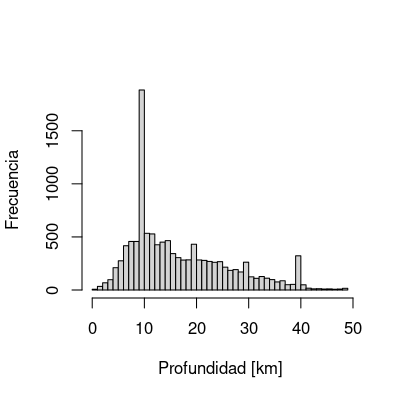
\includegraphics[width=0.4\textwidth]{histograma_profundidad_menos50.png}
  \vspace{-1cm} % Adjust the value as needed
	\caption{Los sismos con origen a mayor profundidad de \SI{50}{\kilo\metre} son mayoritarios en el conjunto de datos.}
	\label{fig:histograma_profundidad750km}
% \end{wrapfigure}
\end{figure}



\subsection{Linealización de la magnitud}\label{sec:linealización}
% \paragraph{Linealización de la magnitud}
Todas las escalas de magnitud buscan dar cuenta de la energía liberada en el terremoto.
La escala utilizada en los datos del INPRES es la de magnitud de momento (ver sección \ref{sec:datos}) definida como \cite[ec. 4.23]{fowler_solid_1990}
\begin{equation}
	M_w =
	\frac{2}{3} \log_{10} \left( M_0 \right) - 6.0 = 
	\frac{2}{3} \log_{10} \left( \mu A u \right) - 6.0,
	\label{eq:momento}
\end{equation}
donde \(M_0\) es el llamado \emph{momento sísmico} a su vez función del módulo de cizalladura, \(\mu\), el área de falla involucrada, \(A\), y su desplazamiento promedio, \(u\), todas características del fenómeno en profundidad \cite*[sección 4.2.4]{fowler_solid_1990}.

Como se discutió en la sección \ref{sec:magnitud} \(M_w\) fue precedida por otras escalas de magnitud ligadas a la amplitud de las ondas sísmicas percibidas en la superficie, como la de onda de cuerpo, \(m_b\), y la de onda superficial, \(M_s\), derivadas de la original de Richter de 1935.
Puesto que este trabajo busca predecir la percepción por personas en la superficie, interesa relacionar los datos de \(M_w\) con estas escalas que tienen una forma genérica
\begin{equation}
	M = \log_{10} \left( \frac{A}{T} \right) + q(\Delta, h) + a,
	\label{eq:magnitud}
\end{equation}
donde \(M\) es la magnitud, y aquí \(A\) es la amplitud de las ondas sísmicas detectadas, \(T\) su período de oscilación, \(q\) es función de la profundidad del hipocentro, \(h\), \(\Delta\) el ángulo entre éste y el sismógrafo y la vertical, y \(a\) es una constante de ajuste \cite[ecuación 4.13]{fowler_solid_1990}.

Dado que se carece del dato del punto de detección del sismo, no puede determinarse \(\Delta\) y aunque se eligiera la escala que corresponde por \(h\) \footnote{Si \(h< \SI{50}{\kilo\metre}\) la mayor parte del aporte a la sismicidad la hacen ondas de propagación superficial por lo que se utiliza la \emph{magnitud de onda superficial}, \(M_s\), con distintos coeficientes de ajuste en la ecuación \ref{eq:magnitud}, que la \emph{magnitud de onda de cuerpo}, \(m_b\), que se usa para mayores profundidades \cite[sección 4.2.3]{fowler_solid_1990}.} no podría determinarse \(q(\Delta, h)\).
Frente a esto las diferencias entre las relaciones empíricas entre \(M_w\) con \(M_s\) o \(m_b\)\cite{hanks_moment_1979}, son irrelevantes a los fines de este trabajo.
Se asume entonces por válida una fuerte aproximación
\begin{equation}
	M_w \approx M_s \approx m_b.
	\label{eq:igualdad}
\end{equation}

Para las ondas de tipo S y P, las que contribuyen a los sismos percibidos en superficie (ver sección \ref{sec:contexto}) se puede hacer uso de la escala propuesta originalmente por Guntenberg en 1945 con la función de calibración para \(q(\Delta, h)\) propuesta por \emph{Gutemberg-Richter} en 1956 \cite[ecuación 4.18]{fowler_solid_1990} en la que se se omite de la expresión \ref{eq:magnitud} la constante de ajuste \(a\) y para definir la razón \(\frac{A}{T}\) se toma la mayor registrada por los sismógrafos,
\begin{equation}
	m_b = \log_{10} \left( \frac{A}{T} \right)_\text{máx} + q(\Delta, h).
	\label{eq:richter}
\end{equation}
Para \(q(\Delta, h)\) se usan valoren tabulados, e.g. para ondas P en \(\Delta = \SIrange{10}{110}{} ^\circ\) corresponden \(q(\Delta, h) \approx \SIrange{6}{8}{}\) \cite{willian_l_ellsworth_earthquake_1991}.

Para obtener un valor lineal \(A\) a partir de la escala \ref{eq:richter}, que es la utilizada en los datos de magnitud del INPRES, se consideró usar una valor medio del rango comentado en el párrafo anterior, \(\overline{q}(\Delta,h)\), con lo que podría despejarse
\begin{equation}
	\left( \frac{A}{T} \right)_\text{máx} = 10^{(m_b - \overline{q}(\Delta,h) )}.
	\label{eq:linealizacionMagnitud}
\end{equation}
Pero la mínima magnitud, hallada con
\begin{lstlisting}[breaklines=true, language=R]
	magnitud_mínima = min(sismos_SJ[,Magnitud, ])
\end{lstlisting}	
resultó ser menor que ese promedio, \(\overline{q}(\Delta,h) = 7\), por lo que si se lo restara se obtendrían valores negativos para el valor a la izquierda de la ecuación y esto sería algo sin validez física (¡amplitudes negativas!).
Se decidió utilizar entonces un ficticio \(\tilde{q}(\Delta,h) = \) \lstinline[language = R]'magnitud_mínima'.  

De querer despejar la amplitud de las ondas, \(A\), debiera tenerse información sobre el período de las ondas, \(T\), algo que no figura en el conjunto de datos.
No se encontró otra alternativa que asumir que todos los fenómenos registrados tienen el mismo y en consecuencia asumir \(T_\text{constante}\).
Así realizando despejes a partir de la ecuación \ref{eq:richter} y asumiendo tales condicionantes, se puede obtener un valor linealmente relacionado con la amplitud registrada por un sismógrafo, \(A_\text{máx}\),
\begin{equation}
	\left( \frac{A_\text{máx}}{T_\text{constante}} \right) = 10^{(m_b - \tilde{q}(\Delta, h))}.
	\label{eq:linealizacionMagnitud_final} 
\end{equation}
Con el comando
%\lstinline[language = R]'
\begin{lstlisting}[breaklines=true, language=R]
sismos_SJ[, Proxy\_amplitud := 10^(Magnitud- magnitud_mínima)]
\end{lstlisting}
%'
se generó una columna para este valor denominada \lstinline[language = R]'Proxy amplitud', que por lo comentado anteriormente tiene por valor mínimo \num{1}. 



\subsection{Percepción sísmica, ¿de amplitud o energía?}
Es posible también que que en el límite entre percepción o no (I o II de la escala MMI \cite{noauthor_intensidad_2022}) pueda explicarse mejor en función de la energía de la onda sísmica que de la amplitud, por lo que podría esperarse una mejor correlación con el cuadrado de esta última variable derivada.
Para ensayarlo se generó con
%\lstinline[language = R]'
\begin{lstlisting}[breaklines=true, language=R]
sismos_SJ[, `Proxy energía` := `Proxy amplitud`^2]
\end{lstlisting}
%' 
la nueva variable \lstinline[language = R]'Proxy energía', 


\section{Variables a correlacionar con la percepción}\label{sec:correlaciones}
De las variables originales, aquellas referidas al momento de detección del sismo, Fecha y Hora, y sus derivadas, Año, Día del año y Segundo del día, no se buscará explorar otra relación con la percepción que la presentado en el análisis exploratorio de datos, sección \ref{sec:AED}.

Restan, por un lado, las variables sobre la localización del terremoto, Latitud, Longitud y Profundidad, independientes entre sí.
Por el otro, la única referida a la física del mismo, la Magnitud, y sus derivadas Proxy amplitud y Proxy energía, que se hipotetiza puede mostrar mejor relación con la percepción si ésta depende de la amplitud o energía de la oscilación sísmica.
% De los datos sobre parámetros físicos del terremoto, Magnitud y Profundidad, se trabajará con la segunda sin modificación, en tanto que se espera un mejor desempeño en modelos que se basen en la variable elaborada a partir de la primera, Proxy\_amplitud por lo expuesto en la sección \ref{sec:ingeniería}.
Como estas tres variables no tienen una relación lineal entre sí, se espera que puedan aportar información independiente al modelo de clasificación.
% De todas formas, como la relación entre ambas no es lineal, la covarianza entre ambas es elevada, \(\approx 0.233\), pero no es perfecta por lo que podría ensayarse el impacto de usar alternativamente Magnitud o Proxy\_amplitud en distintos modelos.

Como una medida preliminar de la valía de cada variable para los fines de clasificación se calcularon sus covarianzas con la variable de percepción.
 comando
\begin{lstlisting}[breaklines=true, language=R]
 cor(sismos_SJ[, .(`Latitud`, `Longitud`, `Magnitud`, `Profundidad`, `Proxy amplitud`, `Proxy energia`, Percibido)])
\end{lstlisting}	
 que generó los valores que muestra el cuadro \ref{tab:correlaciones}. 

\begin{table}[!ht]
	\centering
	\resizebox{\textwidth}{!}{
		\begin{tabular}{llllll}
			\toprule
      Magnitud & Proxy amplitud & Proxy energía & Longitud & Latitud & Profundidad\\ 
			\midrule
			0.40571008 & 0.16537190 &  0.06037060 & 0.05548810 & -0.01035141 & -0.14235874\\
			\bottomrule
		\end{tabular}
	}
	\caption{Covarianzas con la variable Percibido de las otras variables con las que buscará predecirse.}
	\label{tab:correlaciones}
\end{table}

Respecto a la ubicación del terremoto se muestra el esperable resultado que cuanto más profundo menos percibido es.
Menor impacto tiene donde está el epicentro.
La latitud es casi irrelevante, siendo más relevante que cuanto al oeste se detecta un terremoto, esto es, con una mayor longitud, sean más percibidos.
Cuanto más al oeste, se está más adentrado en la cordillera de los Andes, donde menos población se ubica, así que el incremento de la percepción no se debiera a una mayor proximidad entre terremoto y quién lo reporta.
Lo que también cabe esperarse es que allí los terremotos sean de mayor magnitud, por lo que la explicación de la mayor percepción con mayor longitud tendría esta variable como mediadora en la relación.
Sin embargo la correlación entre longitud y magnitud, calculada por
%\lstinline[language = R]'
\begin{lstlisting}[breaklines=true, language=R]
cor(sismos_SJ[, .(`Longitud`,`Magnitud`)], use = "complete.obs")
\end{lstlisting}
%'
de \num{0.008050125}, resulta ser despreciable, lo que lleva a abandonar esta explicación.

La magnitud es la variable que mayor correlación tiene con la percepción de los sismos.
En esto aventaja apreciablemente a las variables sintetizadas a partir de ella, las aproximaciones a la amplitud y energía de las ondas sísmicas.
Puesto que las relaciones de esta últimas con la primera no son lineales, no están perfectamente correlacionadas entre sí, lo que mostró la ejecución de  
\begin{lstlisting}[breaklines=true, language=R]
cor(sismos_SJ[, .(`Magnitud`, `Proxy amplitud`, `Proxy energía`)], use = "complete.obs")
\end{lstlisting}
%'
arrojando que esta es \num{0.2328335} y \num{0.09030076} respectivamente.
Por lo que estas variables no son redundantes entre sí y se espera que aporten información independiente al modelo de clasificación.
Se ensayará retira de entre las variables utilizadas estas variables derivadas para generar distintos modelos y evaluar el impacto de su inclusión.





%de los sismos a analizarán muestra una débil correlación positiva con la variable que depende de la amplitud de las ondas sísmicas y una negativa con la profundidad del terremoto en concordancia con las expectaciones lógicas que pueden tenerse sobre el fenómeno.

%Un orden de magnitud menor hay una positiva con la longitud, lo que se esperaba por acercarse a la cordillera, y una menor en magnitud con la latitud.

%Relativamente la hora a la largo de todo el día no prácticamente correlación con la percepción de los sismos.
%Para analizar esto último hay que segmentar por bandas horarias. 

%se verificó que lo covarianza de Percibido con Hora\_decimal es casi nula, que cuanto más profundo es el terremoto es menos percibido y que era de esperarse que terremotos que liberan más energía sean más percibidos, Magnitud y Proxy\_amplitud muestran una correlación positiva.
% La correlación de la percepción con la latitud resultó ser menos significativa que con la longitud.


\section{Preprocesamiento}


\subsection{Escalamiento}\label{sec:escalamiento}
Previo a la partición (splitting) se realiza un escalado uniforme sobre todo el conjunto de datos (scaling) de las variables numéricas, excluyendo las de fecha y hora con las que no se trabajará de aquí en adelante.
Restando a cada valor de la variable su media y dividiendo por su desviación estándar se obtiene una variable con media cero y desviación estándar uno. 
Esto tiene consecuencias para interpretabilidad del modelo de regresión:
\begin{itemize}
	\item los coeficientes serán comparables entre sí, no dependiendo de la escala de los datos,
	\item el intercepto del modelo será la predicción esperada para el caso en que los factores contemplados sean nulos, es decir, no tengan efecto,
	\item y finalmente si se hace uso de regularización se evita que los coeficientes de las variables de mayor escala tengan un peso desproporcionado en la función de pérdida \cite[sección 3.4.1]{hastie_elements_2009}.
\end{itemize}
Para esto se hace uso de \lstinline[language = R]'scale', función del conjunto base de R, para generar \lstinline[language = R]'sismos_SJ_escalado' con el comando
\begin{lstlisting}[breaklines=true, language=R]
sismos_SJ_escalado <- scale(sismos_SJ[, .(Latitud, Longitud, Profundidad, Magnitud, `Proxy amplitud`, `Proxy energía`)])
\end{lstlisting} 


\subsection{Partición con estratificación}\label{sec:partición}

Dado el fuerte desequilibrio de la clase \texttt{Percibido} comentado en la sección \ref{sec:AED}, ante una división de los datos en subconjuntos entrenamiento (train) y ensayo (test), está el riesgo de que el subconjunto de prueba quede con muy pocos casos positivos y no sea representativo de la distribución de la clase en el conjunto de datos. 
Para evitar esto se realiza una división estratificada, esto es, 
manteniendo en los subconjuntos de entrenamiento y ensayo una proporción similar a la original de los casos de \verb'Percibido'.
Las evaluaciones sobre la calidad de los modelos de clasificación generados se realizarán sobre un subconjuntos de ensayo con el \(20 \%\) de los datos de la provincia de San Juan, el resto se utilizará para el entrenamiento.
aplicando la función \lstinline[language = R]'CreateDataPartion' de la biblioteca \lstinline[language = R]'caret' en el comando

\begin{lstlisting}[breaklines=true, language=R]
set.seed(123)
train_index <- caret::createDataPartition(sismos_SJ_escalado[ , Percibido], p = 0.8, list = FALSE)
entrenamiento_SJ <- sismos_SJ_escalado[train_index]
ensayo_SJ <- sismos_SJ_escalado[-train_index]
\end{lstlisting}

La función mencionada indicó los índices de los datos a incluir en el conjunto de entrenamiento, \lstinline[language = R]'entrenamiento_SJ'.
Los datos restante se destina al conjunto de ensayo, \lstinline[language = R]'ensayo_SJ', este último con un número aún adecuado para su función de \num{5982} registros.


\subsection{Desequilibrio en clase de clasificación}\label{sec:balanceo}
Para contrarrestar el desequilibrio en el conjunto de entrenamiento sobre la clase de clasificación se utilizará la técnica de sobremuestreo de la clase minoritaria que genera nuevos casos sintéticos de la clase minoritaria a partir de los existentes.
Para esto se utiliza la función \lstinline[language = R]'ovun.sample' de la biblioteca \lstinline[language = R]'ROSE' que genera un conjunto de datos de entrenamiento con un número de casos de la clase minoritaria igual al de la clase mayoritaria.
Se generó así un nuevo conjunto de datos de entrenamiento \lstinline[language = R]'entrenamiento_SJ_balanceado' con \num{23934} registros.



% \section{Descripción de los métodos estadísticos utilizados (si corresponde)}


\section{Métricas de evaluación de los modelos}\label{sec:métricas}
% \section{Descripción de las métricas de evaluación de los modelos (si corresponde)}

Independientemente del modelo de clasificación que se utilice, la evaluación de su desempeño se realiza a partir de la comparación de las predicciones del modelo con los valores reales de la variable objetivo.
%Se reservará un subconjunto de los datos para evaluar el desempeño del modelo, el conjunto de prueba y generar una matriz de confusión.


\paragraph{Matriz de confusión}
La matriz de confusión es una tabla que muestra el número de verdaderos positivos, falsos positivos, verdaderos negativos y falsos negativos del modelo.
A partir de esta matriz se pueden calcular como razones entre verdaderos y falso positivos y negativos la exactitud, precisión, sensibilidad, especificidad y el valor F1, entre otras métricas de desempeño.


\paragraph{Exactitud (accuracy)}
La exactitud es la proporción de predicciones correctas sobre el total de casos.
Se calcula como
\begin{equation}
	\text{Exactitud} = \frac{\text{Verdaderos positivos} + \text{Verdaderos negativos}}{\text{Verd. pos.} + \text{Falsos pos.} + \text{Verd. neg} + \text{Falsos neg}}.
\end{equation}


\paragraph{Precisión}
La precisión es la proporción de predicciones correctas sobre el total de predicciones realizadas.
Se calcula como
\begin{equation}
	\text{Precisión} = \frac{\text{Verdaderos positivos}}{\text{Verdaderos positivos} + \text{Falsos positivos}}.
\end{equation}
En este trabajo cuantifica cuantos de las predicciones de percepción de sismos, efectivamente figuraban como tales en el conjunto de datos de ensayo.
Esencialmente es una medida de que cuanto se equivoca la predicción en términos de reportar un evento que se percibirá cuando el publico no lo hizo según lo que figura en el conjunto de datos de ensayo.


\paragraph{Sensibilidad o exhaustividad (recall)}
La sensibilidad, o exhaustividad, es la proporción de verdaderos positivos sobre el total de casos positivos.
Se calcula como
\begin{equation}
	\text{Sensibilidad} = \frac{\text{Verdaderos positivos}}{\text{Verdaderos positivos} + \text{Falsos negativos}}.
\end{equation}
En este trabajo cuantifica cuantos de los terremotos que tendrían que haber producido una predicción de percepción por parte de la población fueron efectivamente reportados como tales por el modelo al ensayarle en el conjunto de ensayo.
Es esencialmente una medida de cuantos reportes falla en realizar.


\paragraph{Especificidad}
La especificidad es la proporción de verdaderos negativos sobre el total de casos negativos.
Se calcula como
\begin{equation}
	\text{Especificidad} = \frac{\text{Verdaderos negativos}}{\text{Verdaderos negativos} + \text{Falsos positivos}}.
\end{equation}


\paragraph{F1-score}
El \emph{F1-score} es la media armónica de la precisión y la sensibilidad (recall).
Se calcula como
\begin{equation}
	\text{F1-score} = 2 \times \frac{\text{Precisión} \times \text{Recall}}{\text{Precisión} + \text{Recall}}.
\end{equation}


%Con un gráfico de estas métricas en función del punto de corte entre clases se elige manualmente aquel que permita clasificar las instancias en una de las dos clases.
%Como complemento se pueden trazar las curvas ROC y PR para evaluar el desempeño de los modelos en separar las clases.
%
%
%\paragraph{Área bajo la curva ROC}
%El área bajo la curva ROC (AUC-ROC) es una métrica que evalúa la capacidad de un modelo de clasificación para discriminar entre clases.
%Se calcula como el área bajo la curva ROC, que es la curva que representa la tasa de verdaderos positivos en función de la tasa de falsos positivos.
%El valor de AUC-ROC varía entre 0 y 1, donde 0 indica un modelo que clasifica todas las instancias de la clase positiva como negativas y viceversa, y 1 indica un modelo que clasifica perfectamente las instancias de ambas clases.
%
%
%\paragraph{Área bajo la curva PR}
%El área bajo la curva PR (AUC-PR) es una métrica que evalúa la capacidad de un modelo de clasificación para discriminar entre clases.
%Se calcula como el área bajo la curva PR, que es la curva que representa la precisión en función del \emph{recall}.
%El valor de AUC-PR varía entre 0 y 1, donde 0 indica un modelo que clasifica todas las instancias de la clase positiva como negativas y viceversa, y 1 indica un modelo que clasifica perfectamente las instancias de ambas clases.



%\paragraph{Validación cruzada}
%La validación cruzada es una técnica que se utiliza para evaluar el desempeño de un modelo de clasificación.
%Consiste en dividir el conjunto de datos en \(k\) subconjuntos, entrenar el modelo en \(k-1\) subconjuntos y evaluarlo en el subconjunto restante.
%Este proceso se repite \(k\) veces, de modo que cada subconjunto se utiliza una vez como conjunto de prueba.
%

% En este trabajo se utilizará la AUC-ROC la utilizada para de los modelos de clasificación ajustados en este trabajo.



\chapter{Resultados y discusión}


% \section{Presentación de resultados}
% \section{Presentación y análisis de resultados obtenidos}


\section{Predictor por regresión logística múltiple}

Como se indicó en la sección \ref{sec:logística} una de las metodologías de predicción fue el de emplear modelos de predicción logísticas.
De acuerdo a cuales de las variables disponibles y que interacciones entre ellas  se incluyen se obtuvieron distintas modelos de clasificación.


\subsection{Todas las variables}\label{sec:logística_sin_interacción}

El primer modelo ensayado tiene todas las variables como predictores sin interacción entre ellas,

\begin{align}
	\log \left( \frac{p}{1-p} \right) = & \beta_0 
	+ \beta_1\, \text{Magnitud} 
	+ \beta_2 \, \text{Proxy amplitud}\notag\\
	& + \beta_3 \, \text{Latitud} 
	+ \beta_4 \, \text{Longitud} 
	+ \beta_5 \, \text{Profundidad} 
	,
	\label{eq:regresion_logistica}
\end{align}

Este modelo se establece gracias a la función \lstinline[language = R]'glm2' (ver sección \ref{sec:logística}) con el comando
\begin{lstlisting}[language=R, breaklines=true]
logit_model <- glm2::glm2(
  Percibido ~ Magnitud + `Proxy_amplitud` + `Proxy_energía` + Longitud + Latitud + Profundidad,
   data = entrenamiento_SJ_balanceado,
  family = "binomial"
  )
\end{lstlisting}
donde la opción \lstinline[language = R]'family = "binomial"' indica que se ajustará un modelo de regresión logística de clasificación binaria sobre la variable \lstinline[language=R]|Percibido| que se muestra en función de las demás en el conjunto de dato indicado con \lstinline[language=R]|data| apuntando al conjunto de entrenamiento balanceado según se explicó en la sección \ref{sec:balanceo}.
Los resultados del ajuste para los coeficientes los muestra una invocación de la función \lstinline[language = R]'summary' que muestra el cuadro \ref{tab:coeficientes}. 

\begin{table}[!ht]
 	\centering
 	\begin{tabular}{lllcc}
 		\toprule
 		Variable & Coeficiente & Error estándar & \(z\) & \(Pr(>|z|)\) \\
 		\midrule
 		Intercepto & -2.232632 & 0.033904 & -65.851 & < 2e-16 \\
 		Magnitud & 1.575057 & 0.020722 & 76.010 & < 2e-16 \\
 		Proxy amplitud & 0.003223 & 0.008529 & 0.378 & 0.706 \\
 		Proxy energía & -0.003303 & 0.008250 & -0.400 & 0.689 \\
 		Longitud & 0.183377 & 0.021651 & 8.470 & < 2e-16 \\
 		Latitud & -0.167088 & 0.021658 & -7.715 & 1.21e-14 \\
 		Profundidad & -0.987883 & 0.017962 & -54.997 & < 2e-16 \\
 		\bottomrule
 	\end{tabular}
 	\caption{Coeficientes del modelo de regresión logística múltiple.}
 	\label{tab:coeficientes}
\end{table}

Excepto los coeficientes para \lstinline[language = R]'Proxy_amplitud' y  \lstinline[language = R]'Proxy_energía', todos son significativos ya que sus probabilidades de que no tengan esos valores y se cumpla la hipótesis nula \(Pr(>|z|)\) para el estadístico \(z = \beta / \sigma_\beta\), se indican como inferiores al umbral usual de \(0.05\).
Para el modelo de predicción a utilizar se optaría por obviar \lstinline[language = R]'Proxy_amplitud' y  \lstinline[language = R]'Proxy_energía'.
Antes de hacerlo y dejar definitivamente de lado las mismas se explorará si se puede mejorar el modelo con la inclusión de interacciones entre las variables.
Estas debieran poder corregir sesgos introducidos al modelo por incluir entre sus variables aquellas supuestamente independientes pero que muestran correlación.

%Así una segunda propuesta de modelo excluyendo \lstinline[language=R]{Proxy_energía}se generó con el comando 
%\begin{lstlisting}[language=R, breaklines=true]
%logit_model_sin <- glm(
%  Percibido ~ Magnitud + `Proxy_amplitud` + Longitud + Latitud + Profundidad,
%   data = entrenamiento_SJ_balanceado,
%  family = "binomial"
%  )
%\end{lstlisting}



\subsection{Interacción entre variables}\label{sec:logística_con_interacción}
Entre las 6 variables numéricas pueden formase pares de interacción, lo que lleva a preguntarse cuales incluir en un modelo.
Puesto que se busca que incluirle aporte a mejorar la predicción por corrección del sesgo que aporta su inclusión sin dar cuenta de la covarianza entre ellas se buscó determinar cuales pares presentan un mayor valor de la misma.

Las covarianzas entre las variables deben volver a calcularse pues estas no son las mismas en el subconjunto de entrenamiento que en el total de los datos.
Aunque la modificación que causa la partición en si no es muy importante (ver sección \ref{sec:partición}), si es más significativa la causada por el posterior balanceo de la clase de clasificación (ver sección \ref{sec:balanceo}).
Se generó una función basada en la ya mencionada \lstinline[language=R]{cor} para determinar los pares de variables con mayor valor absoluto de covarianza.
Las que superan un corte arbitrario de \num{0.03} se muestran en el cuadro \ref{tab:covarianza}, junto con el respectivo valor.

\begin{table}[!ht]
	\centering
	\begin{tabular}{ll}
		\toprule
		Variables & Covarianza\\
		\midrule
		Proxy\_energía - Proxy\_amplitud & 0.7432113838\\
		Proxy\_amplitud - Magnitud & 0.3088276448\\
		Profundidad - Longitud & 0.2930435805\\
		Proxy\_energía - Magnitud & 0.1609778094\\
		Magnitud - Longitud & 0.0427277428\\
		Profundidad - Latitud & 0.0382461548\\
		\bottomrule
	\end{tabular}
	\caption{Covarianza entre pares de variables numéricas.}
	\label{tab:covarianza}
\end{table}
No es de extrañar que figuren las covarianzas entre \verb'Magnitud' y sus derivadas entre las de mayor covarianza.
Pero también figuran unas no esperadas entre \verb'Profundidad' y ubicación del epicentro, además de las más esperadas entre \verb'Magnitud' y \verb'Longitud', por las razones discutidas en la sección \ref{sec:correlaciones}.

Un modelo incorporando todas estas interacciones de pares a aquel propuesto en la sección \ref{sec:logística_sin_interacción} se generó con el comando
\begin{lstlisting}[language=R, breaklines=true]
logit_model_interaccion <- glm2::glm2(
	Percibido ~ Magnitud * `Proxy_amplitud` + Longitud * Profundidad,
	 data = entrenamiento_SJ_balanceado,
	family = "binomial"
	)
\end{lstlisting}

Nuevamente los p-values indican que las variables derivadas de \verb'Magnitud' y las interacciones con las mismas no aportan significativamente al modelo, como muestra el cuadro \ref{tab:coeficientes_interaccion}, pero todas las demás interacciones resultan aportar significativamente al modelo.

\begin{table}
	\centering
	\begin{tabular}{lllcc}
		\toprule
		Variable & Coeficiente & Error estándar & \(z\) & \(Pr(>|z|)\) \\
		\midrule
		Intercepto & -2.265e+00 & 3.527e-02 & -64.221 & < 2e-16 \\
		Magnitud & 1.598e+00 & 2.174e-02 & 73.503 & < 2e-16 \\
		Proxy amplitud & 6.392e-04 & 1.203e-02 & 0.053 & 0.957625 \\
		Proxy energía & -2.872e-03 & 1.188e-02 & -0.242 & 0.808996 \\
		Longitud & 3.211e-01 & 3.213e-02 & 9.994 & < 2e-16 \\
		Latitud & -1.291e-01 & 2.301e-02 & -5.612 & 2.00e-08 \\
		Profundidad & -1.004e+00 & 1.923e-02 & -52.209 & < 2e-16 \\
		Proxy amplitud:Proxy energía & -4.126e-04 & 1.023e-03 & -0.403 & 0.686825 \\
		Magnitud:Proxy amplitud & 1.327e-03 & 5.903e-03 & 0.225 & 0.822178 \\
		Longitud:Profundidad & 6.306e-02 & 1.636e-02 & 3.855 & 0.000116 \\
		Magnitud:Proxy energía & -1.257e-05 & 6.013e-03 & -0.002 & 0.998332 \\
		Magnitud:Longitud & -1.135e-01 & 1.924e-02 & -5.899 & 3.66e-09 \\
		Latitud:Profundidad & 7.633e-02 & 1.326e-02 & 5.756 & 8.63e-09 \\
		\bottomrule
	\end{tabular}
	\caption{Coeficientes del modelo de regresión logística múltiple incorporando la interacción entre variables.}
	\label{tab:coeficientes_interaccion}
\end{table}

Al parecer entonces se tendría un mejor modelo que ajusta mejor a los datos incorporando estas interacciones.
Para afirmar que efectivamente es mejor se necesita utilizar alguna métrica de la bondad del ajuste.



\subsection{Medida de la bondad del ajuste}\label{sec:bondad}
La desviación (del inglés deviance) es una generalización de la suma de cuadrados de los residuos en el ajuste ordinario de cuadrados mínimos a casos donde el mismo se realiza por máxima verosimilitud \cite[sección 7.2]{hastie_elements_2009}.
Con este valor puede calcularse una especie de \emph{pseudo valores de R cuadrado}, como medida de que tan bien el modelo explica la varianza en la variable dependiente.
Para el modelo presentado en la sección \ref{sec:logística_sin_interacción}, que denominaremos ``sin interacción'', se calcula con el comando
\begin{lstlisting}[language=R, breaklines=true]
	pseudo_r2 <- 1 - logit_model$deviance / logit_model$null.deviance
\end{lstlisting}
donde \lstinline[language=R]{logit_model$null.deviance} sería la del modelo con todos su coeficiente \(\beta_i\) nulos. 

Asumiendo que cuanto menor es este pseudo R cuadrado se logró un mejor ajuste debe calcularse para las otras variantes de modelos de regresión logística múltiple hasta ahora propuestas.
La primera es la variante del modelo presentado en la de la sección \ref{sec:logística_sin_interacción} ``limpio'' de las variables derivadas de \verb'Magnitud', que denominaremos ``sin interacción, sin derivadas'', generado con el comando
\begin{lstlisting}[language=R, breaklines=true]
logit_model_limpio <- glm2::glm2(
  Percibido ~ Magnitud + Longitud + Latitud + Profundidad,
   data = entrenamiento_SJ_balanceado,
  family = "binomial"
  )
\end{lstlisting}

El tercer modelo es el presentado en la sección \ref{sec:logística_con_interacción} con las interacciones entre variables, que denominaremos ``con interacción''.
Y el cuarto es el de esta misma sección pero sin las variables derivadas de \verb'Magnitud', que denominaremos ``con interacción, sin derivadas'', que se generó con el comando
\begin{lstlisting}[language=R, breaklines=true]
	logit_pairwise_limpio <- glm2::glm2(
  Percibido ~
    Magnitud +
    Longitud +
    Latitud +
    Profundidad +
    Profundidad * Longitud +
    Magnitud * Longitud +
    Profundidad * Latitud
    ,
   data = entrenamiento_SJ_balanceado,
  family = "binomial"
  )
\end{lstlisting}

A los fines de comparar el pseudo R cuadrado para cada modelo se los resume en el cuadro \ref{tab:pseudo_r2}.
\begin{table}[!ht]
	\centering
	\begin{tabular}{ll}
		\toprule
		Modelo & Pseudo R cuadrado\\
		\midrule
		Sin interacción & 0.5930901\\
		Sin interacción, sin derivadas &  0.5928425\\
		Con interacción &  0.5938916\\
		Con interacción, sin derivadas & 0.5935757\\
		\bottomrule
	\end{tabular}
	\caption{Pseudo R cuadrado para los distintos modelos de regresión logística múltiple.}
	\label{tab:pseudo_r2}
\end{table}

Si bien el modelo ``con interacción'' es el que tiene el mayor pseudo R cuadrado, la diferencia con su variante ``sin derivadas'' que contiene coeficientes que no mostraron ser significativas (ver sección \ref{sec:logística_con_interacción}) llevan a optar entre ambos por el menos complejo.

Con lo anterior se tomó una decisión sobre cual modelo de regresión logística múltiple utilizar para predecir la percepción de los sismos en la provincia de San Juan, pero no se da una respuesta a si ajusta bien a los datos.
Un ensayo específico para la bondad de ajuste de modelos de predicción logísticas es la prueba de Hosmer-Lemeshow. 
Esta prueba compara la frecuencia observada de eventos en subgrupos de predicción con la frecuencia esperada.
Se calculó con el comando
\begin{lstlisting}[language=R, breaklines=true]
	factor_forHL <- as.numeric(entrenamiento_SJ_balanceado$Percibido) - 1
	hl_test <- ResourceSelection::hoslem.test(factor_forHL, fitted(logit_pairwise_limpio))
	print(hl_test)
\end{lstlisting}
arrojando un resultado bastante negativo, un valor p < \num{2.2e-16}.



\subsection{Evaluación de la predicción del modelo logístico}
El desempeño de los modelos se ensaya comparando la predicción con el conjunto de ensayo \verb'ensayo_SJ' generado en la partición estratificada explicada en la sección \ref{sec:partición}.
Como se discutió en la sección \ref{sec:logística}, los modelos de regresión logística múltiple generan una probabilidad de pertenencia a una clase, \(p\).
La predicción de la clase se realiza asignando a la instancia la clase con mayor probabilidad, es decir, si \(p > 0.5\) se asigna a la clase positiva, y si \(p \leq 0.5\) se asigna a la clase negativa. 
Debe entonces definirse este umbral, o punto de corte, entre las clases para clasificar las instancias.
Para orientar tal decisión se armó una función basada a su vez en la función \lstinline[language=R]{confusionMatrix} de la biblioteca \lstinline[language=R]{caret} para calcular las métricas de evaluación de la predicción en todo un rango de puntos de corte.
Las métricas calculadas son las presentadas en la sección \ref{sec:métricas}: exactitud, especificidad, sensibilidad, especificidad y la media armónica de estás dos últimas, la métrica \(F_1\).

Para el modelo favorecido por el análisis de bondad de ajuste (sección \ref{sec:bondad}), el de regresión logística múltiple con interacción entre variables pero sin contemplar las derivadas de \verb'Magnitud', la figura \ref{fig:múltiple_metrics} muestra las métricas de predicción en un rango \SIrange{0.05}{0.95}{} para el punto de corte.

\begin{figure}[!ht]
	\centering
	\input{graphs/múltiple_metrics.tex}
	\vspace{-0.8cm}
	\caption{Métricas de evaluación para definir manualmente el punto de corte entre clases para el modelo de regresión logística múltiple con interacción entre variables, pero excluyendo las derivadas de la magnitud del terremoto.
	}
	\label{fig:múltiple_metrics}
\end{figure}

No es evidente un punto óptimo, la precisión es muy baja para todos los puntos de corte pero ascendente con el punto de corte, pero la sensibilidad empieza a decaer muy rápido a partir de \(\approx 0.6\).
Se decidió entonces tomar el punto de corte en \num{0.6}, en pos de mantener una alta sensibilidad, es decir que al predecir una predicción por la población hay una alta probabilidad de que esto sea así a costa de que no se generen reportes y luego la población perciban el sismo, lo que representa una baja precisión.
Para este punto de corte de \num{0.6} los valores de las métricas se resumen en el cuadro \ref{tab:múltiple_metrics}.

\begin{table}[!ht]
	\centering
	\begin{tabular}{lllll}
	\toprule
	exactitud & sensibilidad & especificidad & precisión & \(F_1\) \\
	\midrule
	\num{0.9281177} & \num{0.8943089} & \num{0.9288274} & \num{0.2087287} & \num{0.3384615}\\
	\bottomrule
	\end{tabular}
	\caption{Métricas de predicción en el conjunto de ensayo del modelo de regresión logística múltiple con interacciones entre variables excluyendo las derivadas de la magnitud del terremoto. Punto de corte en \num{0.6}.
	}
	\label{tab:múltiple_metrics}
\end{table}

Se repite el análisis de las métricas de evaluación para el modelo con interacción entre variables y que no descarta las variables derivadas de la magnitud.
La figura que muestra las métricas de la predicción en función del punto de corte para este caso, figura \ref{fig:múltiple_metrics_derivadas}, podría decirse que es una copia de la que realizada para el del modelo sin las derivadas de la magnitud, figura \ref{fig:múltiple_metrics}.
Las diferencias son mínimas y esto es un testimonio del poco peso de los coeficientes correspondientes a las variables derivadas de la magnitud, a las relaciones con las otras, en este modelo. 

\begin{figure}[!ht]
	\centering
	\input{graphs/múltiple_derivadas.tex}
	\vspace{-0.8cm}
	\caption{Métricas de evaluación para definir manualmente el punto de corte entre clases para el modelo de regresión logística múltiple con interacción entre variables, incluyendo las derivadas de la magnitud del terremoto.
	Esta figura es a primera vista una copia de la figura \ref{fig:múltiple_metrics_derivadas}, pero los valores de las métricas son ligeramente distintos.
	}
	\label{fig:múltiple_metrics_derivadas}
\end{figure}

Por lo visto en la figura \ref{fig:múltiple_metrics_derivadas} se decidió tomar el mismo punto de corte en \num{0.6} para este modelo.
Los valores de las métricas para este punto de corte también son muy similares a las del otro modelo, como muestra el cuadro \ref{tab:múltiple_metrics_derivadas}.
El desempeño de predicción es marginalmente mejor en este modelo en términos de sensibilidad y precisión, pero éste último sigue siendo muy bajo.

\begin{table}[!ht]
	\centering
	\begin{tabular}{lllll}
		\toprule
		exactitud & sensibilidad & especificidad & precisión & \(F_1\) \\
		\midrule
		\num{0.9282849} & \num{0.8943089} & \num{0.9289981} & \num{0.2091255} & \num{0.3389831}\\
		\bottomrule
	\end{tabular}
	\caption{Métricas de predicción en el conjunto de ensayo del modelo de regresión logística múltiple con interacciones entre variables incluyendo las derivadas de la magnitud del terremoto. Punto de corte en \num{0.6}.
	}
	\label{tab:múltiple_metrics_derivadas}
\end{table}




\section{Predictor por XGBoost}
% \textcolor{red}{Esto es un placeholder para una sección aún vacía.}
Como alternativa a los modelos de regresión logística múltiple, se ajustaron modelos de clasificación con el algoritmo XGBoost.
Se entrenó en primer lugar un modelo con todas las variables disponibles, sin interacción entre ellas, con el comando
\begin{lstlisting}[language=R, breaklines=true]
num_feat = c("Latitud", "Longitud", "Magnitud", "Profundidad", "Proxy_amplitud", "Proxy_energía")
entrenamiento_SJ_balanceado_matrix <- as.matrix(entrenamiento_SJ_balanceado[ ,..num_feat])
label_numeric <- as.numeric(entrenamiento_SJ_balanceado[, Percibido]) - 1
bstSparse <- xgboost(
  data = entrenamiento_SJ_balanceado_matrix, 
  label = label_numeric, 
  max.depth = 5, eta = 1, 
  nthread = 2, nrounds = 5, 
  objective = "binary:logistic", 
  verbose = 2
  )
\end{lstlisting}
donde se indica que se ajustará un modelo de clasificación binaria con la función de pérdida logística, con un máximo de 5 niveles en los árboles y 5 iteraciones.
Estos parámetros fueron elegidos a través de sucesivas pruebas manuales un búsqueda de maximizar la métrica F1 (ver sección \ref{sec:métricas}) al contrastar la predicción, con un umbral de \num{0.5} contra el conjunto de ensayo \verb'ensayo_SJ' generado en la partición estratificada explicada en la sección \ref{sec:partición} con el comando
\begin{lstlisting}[language=R, breaklines=true]
ensayo_SJ_matrix <- as.matrix(ensayo_SJ[ ,..num_feat])
prediction_xgboost <- predict(bstSparse, ensayo_SJ_matrix)
umbral_p = 0.5
prediction_xgboost_binario <- ifelse(prediction_xgboost > umbral_p, 1, 0)
\end{lstlisting}
Para este modelo con todas las variables, incluso los anteriormente deprecadas derivadas de la \verb'Magnitud', las métricas de evaluación de la predicción del modelo con el punto de corte en \(0.5\) que se resumen en el cuadro \ref{tab:xgboost_metrics}.
\begin{table}[!ht]
	\centering
	\begin{tabular}{lllll}
	\toprule
	exactitud & sensibilidad & especificidad & precisión & F1 \\
	\midrule
	\num{0.9804413} & \num{0.1138211} & \num{0.9986346} & \num{0.6363636} & \num{0.1931034} \\
	\bottomrule
	\end{tabular}
	\caption{Métricas de evaluación para el mejor modelo de XGBoost hallado para todas las variables y punto de corte en \(0.5\).}
	\label{tab:xgboost_metrics}
\end{table}

El siguiente ensayo fue con el modelo de regresión logística múltiple sin las variables derivadas de la \verb'Magnitud', que se entrena con un comando en todo similar al anterior a excepción de los cambios
\begin{lstlisting}[language=R, breaklines=true]
num_feat = c("Latitud", "Longitud", "Magnitud", "Profundidad")
... 
  max.depth = 3, eta = 1, 
\end{lstlisting}
donde el número de niveles en los árboles se redujo a 3 y se mantuvo el resto de los parámetros, lográndose un mejor desempeño en predecir en el conjunto de ensayo, como se muestra en el cuadro \ref{tab:xgboost_metrics_sin_derivadas}.

\begin{table}[!ht]
	\centering
	\begin{tabular}{lllll}
	\toprule
	exactitud & sensibilidad & especificidad & precisión & \(F_1\) \\
	\midrule
	\num{0.9222668} & \num{0.8943089} & \num{0.9228537} & \num{0.1957295} & \num{0.3211679} \\
	\bottomrule
	\end{tabular}
	\caption{Métricas de evaluación para el mejor modelo de XGBoost hallado solo con las variables originales y punto de corte en \(0.5\).}
	\label{tab:xgboost_metrics_sin_derivadas}
\end{table}

Se aprecia de comparar los cuadros \ref{tab:múltiple_metrics} y \ref{tab:xgboost_metrics_sin_derivadas} que el modelo de regresión logística múltiple sin las variables derivadas de la \verb'Magnitud' sacrifica la precisión por una mayor sensibilidad, es decir que al predecir que la población percibirá un sismo hay una alta probabilidad de que esto sea así a costa de que muchos reporten no se efectúen y la población perciba sismos, lo que representa una baja precisión.
Se considera que una mayor sensibilidad es más importante a los fines de no emitir una alerta incorrecta a la población de que percibirán un sismo, por lo que se opta por este último modelo de XGBoost para predecir la percepción de sismos en la provincia de San Juan. 



%\subsection{Métricas de XGBoost en función del umbral de corte}
%La elección de la variante del modelo de la sección anterior se basó en la comparación de las métricas de evaluación para un punto de corte en \(0.5\).
%Para evaluar si se puede mejorar la predicción del modelo, se graficaron las métricas de evaluación en función del punto de corte entre las clases, como se muestra en la figura \ref{fig:xgboost_metrics}.




\section{Relevancia de los resultados}
% \section{Discusión de los resultados y su relevancia}
% \textcolor{red}{Esto es un placeholder para una sección aún vacía.}

De los cuatros modelos evaluados para la predicción de la percepción de los sismos en la provincia de San Juan, cual se elija depende de los objetivos de la predicción.

Si se considera que una mayor sensibilidad es más importante a los fines de no emitir una alerta incorrecta a la población de que percibirán un sismo, lo que se busca es una alta sensibilidad, aún a costa de que no se produzcan algunos reportes y aún así la población perciba sismos, lo que representa una baja precisión.
En ese caso tanto el modelo de regresión logística múltiple con o sin las variables derivadas de la \verb'Magnitud', así como el de XGBoost sin estas variables resultan los más adecuados.
Como resume el cuadro \ref{tab:metricas_modelos}, todos estos tienen la misma alta sensibilidad, aunque al precio de una pobre precisión.

\begin{table}[!ht]
	\centering
	\begin{tabular}{llllll}
	\toprule
	Modelo & exactitud & sensibilidad & especificidad & precisión & \(F_1\) \\
	\midrule
	LOrig & \num{0.9281177} & \num{0.8943089} & \num{0.9288274} & \num{0.2087287} & \num{0.3384615}\\
	LDer & \num{0.9282849} & \num{0.8943089} & \num{0.9289981} & \num{0.2091255} & \num{0.3389831}\\
	XOrig & \num{0.9222668} & \num{0.8943089} & \num{0.9228537} & \num{0.1957295} & \num{0.3211679} \\
	XDer & \num{0.9804413} & \num{0.1138211} & \num{0.9986346} & \num{0.6363636} & \num{0.1931034} \\
	\bottomrule
	\end{tabular}
	\caption{Métricas de predicción de los modelos seleccionados. Los modelos seleccionados fueron los de regresión logística múltiple contemplando interacciones entre pares de variables incluyendo las variables derivadas de la magnitud del terremoto (LDer) o sin estas (LOrig), y los de XGBoost, también con (XDer) o sin estas variables derivadas (XOrig).}
	\label{tab:metricas_modelos}
\end{table}

Si por el contrario se busca generar una alerta de que un terremoto será percibido como un sismo por la población, aunque esta resulte luego en una ``falsa alarma'', debe optarse por un modelo que tenga una alta precisión, aún a costa de una baja sensibilidad.
Entre los modelos evaluados, el de XGBoost con todas las variables, incluyendo las derivadas de la \verb'Magnitud', es el que tiene la mayor precisión, como se muestra en el cuadro \ref{tab:metricas_modelos}, aunque sacrifica para esto la sensibilidad.




\section{Limitaciones y posibles mejoras}
% \textcolor{red}{Esto es un placeholder para una sección aún vacía.}
El mayor inconveniente enfrentado es la carencia de algún dato sobre la ubicación del reporte de percepción del sismo, ya discutido en la sección \ref{sec:geográfico}, como ``el problema de la distancia''.
Sumada esta ubicación para los reportados por la población, junto con la de un sismógrafo indicado como el que responsable primario para determinar magnitud y profundidad en los casos de terremotos percibidos o no, podrían hacerse inferencias en base a la distancia.
Incluso sería posible calcular una aproximación al ángulo entre sismógrafo y terremoto y así aplicar la relación correcta entre magnitud y amplitud de onda (ver sección \ref{sec:linealización}).

Algo que resta estudiar es la distribución de la proporción de percepción en función de la estación en el año, pues lo hallado en la sección \ref{sec:temporal} contradijo la hipótesis allí planteada.
Se puede trabajar en la segmentación de los terremotos en trimestres por todos los años como se comenta allí. 



\chapter{Conclusión}

\section{Resumen de los hallazgos principales}
% \textcolor{red}{Esto es un placeholder para una sección aún vacía.}
Se hallaron dos familias de modelos que predicen la percepción por parte de la población de sismos en la provincia de San Juan, Argentina.
Se utilizaron para esto datos públicos de sismos y reportes de percepción de la población publicados por el INPRES.
No se pudo hallar un modelo que conjugue precisión y sensibilidad por lo que de aplicarse uno de ellos hay que optar a cuál de las métricas se le da primacía.


\section{Conclusiones generales y su relación con los objetivos del trabajo}
%\textcolor{red}{Esto es un placeholder para una sección aún vacía.}
En relación a los objetivos planteados en la sección \ref{sec:objetivo}, debe admitirse que si bien pudieron producirse modelos de predicción de la percepción de sismos, esto se logró solo para una provincia en particular por limitación de los datos geográficos disponibles.
Pero la mayor limitación a los modelos de predicción hallados es que no se logró un modelo de aplicación a múltiples problemas, que conjugue precisión y sensibilidad, por lo que de aplicarse uno de los modelos desarrollados hay que optar a cuál de las métricas se le da primacía. 



\section{Aplicaciones y relevancia de los resultados}
%\textcolor{red}{Esto es un placeholder para una sección aún vacía.}
Los modelos desarrollados que mostraron alta sensibilidad, pero baja precisión, pueden ser útiles si las autoridades quieren mostrar a la población de que los terremotos son monitoreados y que se ponen a los sistemas gubernamentales en alerta.
Pueden emitirse alertas de que un terremoto será percibido como un sismo por la población, y habrá una baja probabilidad de que esto resulte en una ``falsa alarma''.

Por el contrario el modelo con alta precisión y baja sensibilidad, al cometer menos errores sobre si un terremoto debiera ser percibido como sismo por la población puede ser útil, no para emitir alerta, pero sí para contrastar con los reportes de percepción de la población y así determinar si hay un faltante de ellos.
Con esto se puede determinar si hay un problema en los sistemas que reciben reportes de percepción de sismos.


% \backmatter

%% bibliografía
% \printbibliography[heading=bibnumbered] % numbered as chapter
\printbibliography[heading=bibintoc] % not numbered

% Bibliografía:
% Referencias bibliográficas citadas en el documento
% Otras fuentes consultadas


\chapter*{Anexos (opcionales)}
\addcontentsline{toc}{chapter}{Anexos (opcionales)}


\section{Código fuente utilizado en el análisis}
Enlace al \href{https://github.com/bettachini/tallerTesis/tree/main/sismosURL}{repositorio en GitHub} que aloja el código fuente utilizado en el análisis de los datos.
% \textcolor{red}{Esto es un placeholder para una sección aún vacía.}



%\section{Tablas y gráficos adicionales}
%\textcolor{red}{Esto es un placeholder para una sección aún vacía.}
%
%
%\section{Otros materiales relevantes}
%\textcolor{red}{Esto es un placeholder para una sección aún vacía.}


\end{document}
